%%%%%%%%%%%%%%%%%%%%%%%%%%%%%%%%%%%%%%%%%%%%%%%%%%%%%%%%%%%%%%%%%%%%%%%%%%%%%%%%
% \documentclass[12pt,papel,twoside]{ibtesis}
\documentclass[12pt,screen,twoside]{ibtesis}
% \documentclass[12pt,papel,singlespace,oneside]{ibtesis}
% \documentclass[12pt,papel,preprint,singlespace,oneside]{ibtesis}


%%%%%%%%%%%%%%%%%%%%% Paquetes extra %%%%%%%%%%%%%%%%%%%%%%%%%%%%%%%%%%%%%%%%%%%
% Por conveniencia: aqu\'{\i} puede cargar todos los paquetes y definir los comandos 
% que necesite
%\usepackage{ibextra}

\usepackage[utf8]{inputenc}
\usepackage[T1]{fontenc}             % evita problemas con á/é/ñ en PDF
\usepackage[spanish, english]{babel} % orden = idioma principal primero
\usepackage[dvipsnames]{xcolor} %Si quisieramos poner texto en color
\usepackage{float} %para poner Here en imagen
\usepackage{graphicx} %para insertar imágenes
\usepackage{subfig}
\usepackage{amsfonts}
\usepackage{amsmath}
\usepackage{mathtools}
\usepackage{comment}
\usepackage{xcolor}  
\usepackage{amssymb}
\usepackage{booktabs}
\usepackage{hyperref}
%\usepackage{ibextra}
                % Archivo de bibliografía


%%%%%%%%%%%%%%%%%%%%%%%%%%%%%%%%%%%%%%%%%%%%%%%%%%%%%%%%%%%%%%%%%%%%%%%%%%%%%%%%
%%%%%%%%%%%%%%%%%%%%% Informacion sobre la tesis %%%%%%%%%%%%%%%%%%%%%%%%%%%%%%%
\title{Análisis del Flujo en Convección Mixta en Canales Rectangulares}
\author{Patricio G. Canciani}
\director{Dr. William I. Machaca Abregu}
\codirector{Dr. Federico Teruel}
\carrera{Tesis Carrera de Maestría en Ingeniería}
\grado{Maestrando}
\laboratorio{Departamento de Mecánica Computacional \\ (Centro Atómico Bariloche)}
\jurado{Dr. Christian P. Marcel (Instituto Balseiro -- CNEA)\\ 
Dr. Pablo Garcia Martinez (Instituto Balseiro -- CNEA)\\ 
Dr. César Venier (FCEIA -- SIMEC)\\}

%\palabrasclave{Flujo Turbulento,Convección Mixta}
%\keywords{Turbulent Flow, Mixed Convection}
% Si queremos poner la fecha manualmente:
% \date{Diciembre de 2099}

%%%%%%%%%%%%%%%%%%%%%%%%%%%%%%%%%%%%%%%%%%%%%%%%%%%%%%%%%%%%%%%%%%%%%%%%%%%%%%%%
%\titlepagefalse % Si no quiere compilar la portada descomente esta linea
%\includeonly{apendices} % Compilar s\'{o}lo estos archivos 
\graphicspath{{figs/}} % Lugar donde encontrar las figuras generales (se puede poner uno en cada cap{\'{\i}}tulo)
%%%%%%%%%%%%%%%%%%%%%%%%%%%%%%%%%%%%%%%%%%%%%%%%%%%%%%%%%%%%%%%%%%%%%%%%%%%%%%%%


\begin{document}

% Dentro del environment 'preliminary' va:
% la dedicatoria, resumen, abstract, indices

\begin{preliminary}

% Escriba su dedicatoria
\dedicatoria{
%A mis padres\\
%A mi hermana\\
%A mis amigos\\
A todos mis seres queridos}

%%% \'{I}ndices %%%%

\begin{abreviaturas}
\begin{itemize}
\small{

\item[] $\rho$: densidad del fluido 
\item[] $\mu$: viscosidad cinemática del fluido 
\item[] $\nu$: viscosidad dinámica del fluido
\item[] $\alpha_{T}$: difusividad térmica del fluido 
\item[] $k$: conductividad térmica 
\item[] $c_p$: calor específico a presión constante 
\item[] $q''_w$: flujo de calor en la pared 
\item[] $X,Y,Z$: direcciones de coordenadas cartesianas 
\item[] $x,y,z$: variables de coordenadas cartesianas 
\item[] $t$: tiempo 
\item[] $d$: semiancho del canal 
\item[] $\mathbf{u}$: campo vectorial de velocidades 
\item[] $\text{p}$: campo escalar de presiones 
\item[] $T$: campo escalar de temperaturas 
\item[] $\mathbf{g}$: vector aceleración de la gravedad
\item[] $g$: magnitud de la acelaración gravitacional 
\item[] $L_x,L_y,L_z$: dimensiones del dominio de simulación 
\item[] $\theta$: temperatura transformada por cambio de variable ($\langle T_w \rangle - T$)

\item[] $U_o$: velocidad en el centro del canal 
\item[] $U_b$: velocidad \textit{bulk} 
\item[] $\mathcal{A}$: constante relacionada a la temperatura en la pared (véase Apéndice \ref{apen:constante-A}) 

\item[] Re: número de Reynolds
\item[] Pr: número de Prandtl
\item[] Ri: número de Richardson
\item[] Ra: número de Rayleigh
\item[] Nu: número de Nusselt
\item[] $f$: factor de fricción de Darcy


\item[] $\alpha,\beta$: número de onda en la dirección $X$ y $Z$ 
\item[] $c$: velocidad de fase
\item[] $\omega$: frecuencia angular

\item[] $\kappa$ o TKE: Energía Cinética Turbulenta

\item[] $\tau_w$: tensión de corte en la pared 

\item[] $(\text{.})_w$: magnitudes evaluadas en la pared
\item[] $\langle \text{.} \rangle$: promedio estadístico en la dirección $X$ y $Z$ y/o en el tiempo
\item[] $(\text{.})_b$: magnitudes en \textit{bulk}
%\item[] $\widetilde{(\text{.})}$: indica perturbación asociada a cierta magnitud
%\item[] $\widehat{(\text{.})}$: indica amplitud de una perturbación
\item[] $(\text{.})^{\prime}$: indica fluctuación de cierta magnitud

\item[] $(\text{.})^{*}$: forma adimensional de magnitudes empleando $d$, $U_o$ y $\mathcal{A} \hspace{0.1mm} d$ 
\item[] $(\text{.})^{\star}$: forma adimensional de magnitudes empleando $d$, $U_b$ y $\text{Re} \hspace{0.1mm} \text{Pr} \hspace{0.1mm} \mathcal{A} \hspace{0.1mm} d $ 
\item[] $(\text{.})^{+}$: forma adimensional de magnitudes empleando $d$, $u_{\tau}$ y $T_{\tau}$
\item[] $(\text{.})_{\tau}$: indica unidades de fricción




% SIGLAS
\item[] DNS: \textit{Direct Numerical Simulation}
\item[] PBC: \textit{Periodic Boundary Conditions} 
\item[] MBC: \textit{Mixed Boudary Condition}
\item[] RANS: \textit{Reynolds Averaged Navier-Stokes Equations}
\item[] XC3D: abreviatura de Xcompact3D
\item[] OSMC: \textit{Orr-Sommerfeld Mixed Convection}
\item[] RHS: \textit{Right Hand Side}
\item[] RLS: \textit{Left Hand Side}
\item[] RMS o rms: \textit{Root Mean Square}

}
\end{itemize}
\end{abreviaturas}

\tableofcontents                %\'{I}ndice
%\listoffigures                  %Figuras

%\listoftables                   %Tablas

\begin{resumen}%

La convección mixta en conductos verticales está presente en numerosos sistemas de interés, entre ellos los intercambiadores de calor. Estos sistemas pueden presentar cambios de régimen (laminar-turbulento) durante su funcionamiento. Esto es relevante ya que el coeficiente de fricción ($f$) o el número de Nusselt (Nu) pueden experimentar grandes variaciones. En el presente trabajo se estudia la evolución temporal de magnitudes de interés durante la transición desde el régimen laminar hacia el turbulento, para un canal vertical de placas paralelas con flujo de calor constante en las paredes.

Para estudiar la transición temporal, primero resulta necesario conocer el estado inicial laminar y el estado final turbulento. En ese sentido, se analiza el flujo turbulento completamente desarrollado bajo la influencia de la fuerza boyante. Tanto el estudio del estado turbulento desarrollado como la transición temporal laminar-turbulenta se realiza mediante simulaciones DNS empleando Xcompact3D. 

Las condiciones iniciales que inducen la inestabilidad se obtienen mediante análisis de estabilidad lineal, resolviendo el problema de autovalores y autofunciones derivado de las ecuaciones de Orr-Sommerfeld para convección mixta. Esta resolución se realiza con la herramienta OSMC desarrollada en el grupo MECOM. Las soluciones permiten desencadenar la transición para examinar su evolución temporal. 


En el análisis del régimen turbulento desarrollado se consideran $2100 \leq \mathrm{Re}_o \leq 5000$ \textcolor{black}{(número de Reynolds basado en el semiancho del canal y la velocidad en el centro)}, \linebreak $\mathrm{Pr}=0\text{.}071,0\text{.}71$ \textcolor{black}{(número de Prandtl)} y $0\text{.}04 \leq \mathrm{Ri}_b \leq 106\text{.}5$  \textcolor{black}{(número de \linebreak Richardson  basado en el ancho del canal y la velocidad \textit{bulk})}. Para $\mathrm{Re}_o=5000$ y $\mathrm{Pr}=0\text{.}71$ se  analizan perfiles de cantidades medias y fluctuaciones. Las estimaciones de Nu  concuerdan con correlaciones de la literatura en los rangos estudiados. \textcolor{black}{Se identifica una región del número de boyancia ($10^{-6} \lesssim \text{Bo} \lesssim 3 \times 10^{-5}$), el cual cuantifica la relación entre las fuerzas boyantes y la fuerza impulsora de la convección forzada,} donde Nu disminuye respecto de la convección puramente forzada, asociado a una menor producción de turbulencia próxima a las paredes. Se propone asimismo una correlación empírica para el factor de Darcy ($f$) con buen acuerdo frente a datos y referencias.

La transición laminar-turbulenta se examina para $\mathrm{Re}_o=5000$, $\mathrm{Pr}=0\text{.}71$ y dos intensidades de boyancia ($\mathrm{Ri}_b=0\text{.}04$ y $\mathrm{Ri}_b=1\text{.}06$). Se identifican combinaciones de perturbaciones que inducen la transición y se observa que una mayor boyancia incrementa la inestabilidad del flujo. Las cantidades TKE \textcolor{black}{(Energía Cinética Turbulenta)}, varianza de temperatura, Nu y $f$ muestran respuestas transitorias no monótonas; en el caso de mayor $\mathrm{Ri}_b$ se registra una caída pronunciada de Nu concurrente con aumento de TKE y el aplanamiento del perfil de velocidad por efecto de la turbulencia. Finalmente, se observa que el valor del estado turbulento desarrollado de $\mathrm{Re}_\tau$ \textcolor{black}{(número de Reyndols de fricción)} se encuentra por encima del valor asociado al estado inicial en el caso de $\mathrm{Ri}_b$ menor y por debajo en el de $\mathrm{Ri}_b$ mayor.

\end{resumen}


\begin{abstract}%

Mixed convection in vertical ducts is present in numerous systems of interest, including heat exchangers. These systems may undergo regime changes (laminar–turbulent) during operation. This is relevant since the friction coefficient ($f$) or the Nusselt number (Nu) may exhibit large variations. In the present work, the temporal evolution of quantities of interest is studied during the transition from the laminar regime to the turbulent one, for a vertical parallel-plate channel with constant wall heat flux.

To investigate the temporal transition, it is first necessary to characterize both the initial laminar state and the final turbulent state. In this regard, the fully developed turbulent flow under the influence of buoyancy is analyzed. Both the study of the developed turbulent state and the laminar–turbulent temporal transition are carried out through DNS simulations using Xcompact3D. 

The initial conditions that trigger the instability are obtained by means of linear stability analysis, solving the eigenvalue and eigenfunction problem derived from the Orr–Sommerfeld equations for mixed convection. This resolution is performed with the OSMC tool developed in the MECOM group. The solutions allow the transition to be triggered in order to examine its temporal evolution. 



In the analysis of the developed turbulent regime, $2100 \leq \mathrm{Re}_o \leq 5000$ \textcolor{black}{(Reynolds number based on the channel half-width and the centerline velocity)}, \linebreak $\mathrm{Pr}=0\text{.}071,0\text{.}71$ \textcolor{black}{(Prandtl number)} and $0\text{.}04 \leq \mathrm{Ri}_b \leq 106\text{.}5$ \textcolor{black}{(Richardson number based on the channel width and the bulk velocity)} are considered. For $\mathrm{Re}_o=5000$ and $\mathrm{Pr}=0\text{.}71$, mean and fluctuating quantities are analyzed. The estimates of Nu agree with correlations from the literature within the studied ranges. \textcolor{black}{A region of the buoyancy number ($10^{-6} \lesssim \text{Bo} \lesssim 3 \times 10^{-5}$), which quantifies the relationship between buoyancy forces and the driving force of forced convection,} is identified where Nu decreases with respect to purely forced convection, associated with a lower turbulence production near the walls. An empirical correlation for the Darcy friction factor ($f$) is also proposed, showing good agreement with data and references.

The laminar–turbulent transition is examined for $\mathrm{Re}_o=5000$, $\mathrm{Pr}=0\text{.}71$, and two buoyancy intensities ($\mathrm{Ri}_b=0\text{.}04$ and $\mathrm{Ri}_b=1\text{.}06$). Combinations of perturbations that induce transition are identified, and it is observed that higher buoyancy increases the flow instability. The TKE \textcolor{black}{(Turbulent Kinetic Energy)}, temperature variance, Nu, and $f$ exhibit non-monotonic transient responses; in the case with higher $\mathrm{Ri}b$, a sharp decrease in Nu is recorded, concurrent with an increase in TKE and a flattening of the velocity profile due to turbulence. Finally, it is observed that the value of the developed turbulent-state $\mathrm{Re}\tau$ \textcolor{black}{(friction Reynolds number)} lies above the value associated with the initial state for the lower $\mathrm{Ri}_b$ case and below for the higher $\mathrm{Ri}_b$ case.


\end{abstract}



%%% Local Variables: 
%%% mode: latex
%%% TeX-master: "template"
%%% End: 


\end{preliminary}


% Podemos usar cualquiera de los dos comandos: \input o \include para incluir el texto
\chapter{Introducción}
\label{intro}
%\chapterquote{Hablaban siempre de dinero y planeaban asaltar un banco}{Domingo Cavallo, 2001}

Capitulo introductorio de la tesis


Algunas preguntas clave que deberian responderse en este capitulo:

¿Cuál es el campo general de estudio de tu tesis?

¿Qué fenómeno, problema o sistema estás investigando?

¿Por qué este tema es relevante científica o tecnológicamente?

¿Qué problema específico intenta resolver tu tesis?

¿Cuáles son los objetivos (generales y/o específicos)?

¿Qué enfoque metodológico utilizás? ¿Experimental, teórico, computacional?

¿Cómo está organizada la tesis?

\newpage
\section{Introducción}

Un fluido, en virtud de su masa y velocidad, puede transportar momento. Además, en virtud de su temperatura, puede transportar calor. Estrictamente hablando, la convección es el transporte de energía debido al movimiento global de un medio. Sin embargo, en ingeniería es común utilizar el término convección de forma más amplia para describir la transferencia de calor desde una superficie hacia un fluido en movimiento cuando ambos están a diferentes temperaturas \cite{cengelheat,incropera}. 

La transferencia de calor por convección puede clasificarse según la naturaleza del flujo. Hablamos de convección forzada cuando el flujo es provocado por actores externos como puede ser la acción de bombeo o un gradiente de presión; en cambio, en la convección natural, el flujo es inducido por fuerzas boyantes o de flotación, las cuales se deben a diferencias de densidad producidas por variaciones de temperatura en el propio fluido (Figura \ref{fig:natural_forzada}).

\begin{figure}[H]
 \centering
    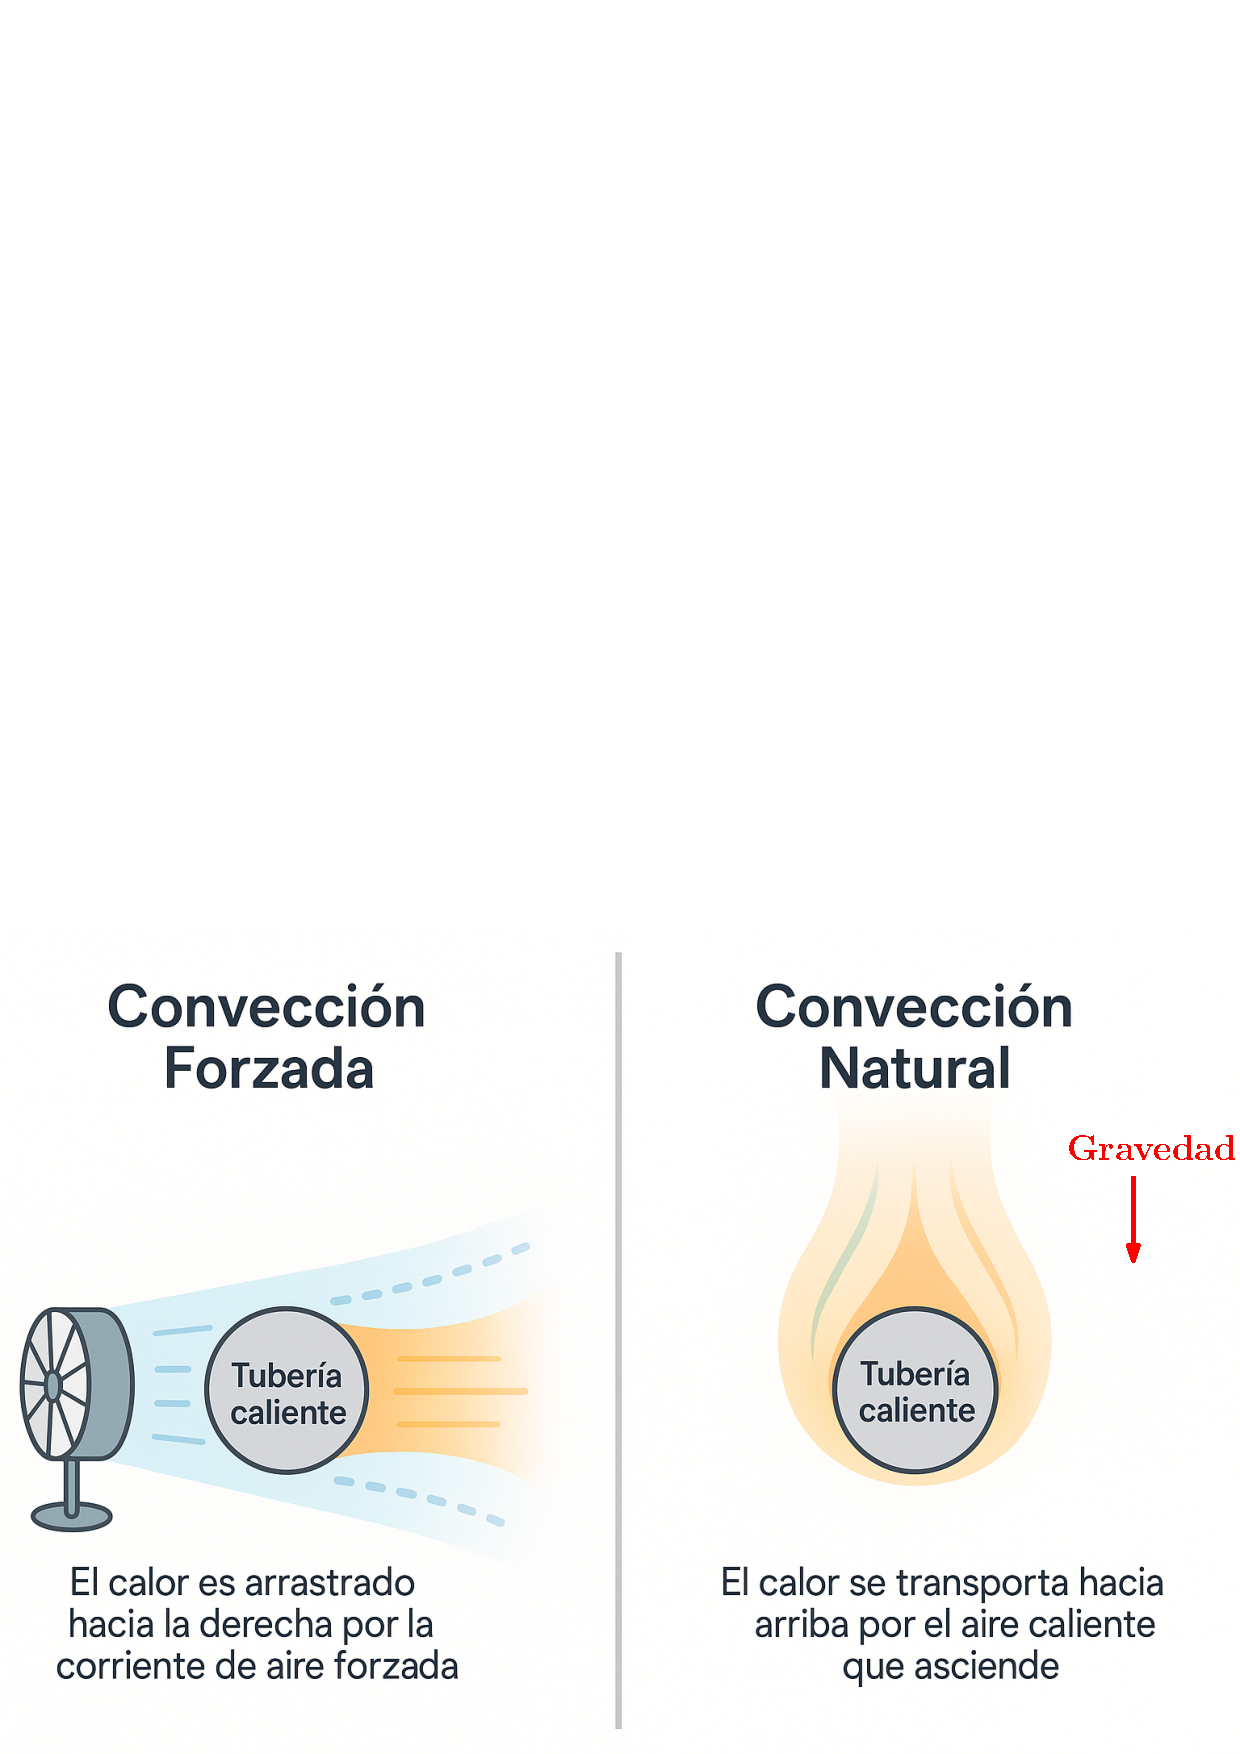
\includegraphics[width=0.6\textwidth]{figures/cap1/natural_forzada.png}
    \label{fig:natural_forzada} 
 \caption{Comparación esquemática de la transferencia de calor alrededor de una tubería caliente: (izquierda) convección forzada; (derecha) convección natural.} 
 \label{fig:natural_forzada}
\end{figure}


Los primeros estudios sobre la transferencia de calor por convección trataron las ramas de la convección forzada y la convección natural de forma separada, sin considerar la posible interacción entre ambas. Por un lado, los experimentos de Henri Bénard (1901) marcaron un hito en la comprensión de la convección natural \cite{benard1901}. Más tarde, Lord Rayleigh (1916) desarrolló la base teórica de la inestabilidad térmica en capas fluidas \cite{rayleigh1916}. En paralelo, en el ámbito de la convección forzada, trabajos como el de Dittus y Boelter (1930) establecieron correlaciones empíricas para la transferencia de calor en tubos \cite{dittus1930}. No fue sino hasta mediados del siglo XX que comenzó a reconocerse que ambos mecanismos pueden coexistir en muchas configuraciones de interés práctico. Así surgió el concepto de convección mixta, donde la convección forzada y la natural actúan simultáneamente como casos extremos de un fenómeno más general \cite{tao1960,metais1964}. 

Por otra parte, cuando un fluido se desplaza a través de un conducto o sobre una superficie, su movimiento puede clasificarse en dos tipos de régimen: laminar o turbulento. En el régimen laminar, el flujo es ordenado y las partículas del fluido se mueven en capas paralelas sin mezclarse entre sí. En cambio, en el régimen turbulento, el flujo es caótico, con remolinos, mezclas intensas y fluctuaciones en velocidad y presión. Un flujo se encuentra en un estado de transición desarrollado (esto es, no varía con el tiempo o con el espacio en un sentido de promedio estadístico), se dice que el flujo está en régimen de transición. Por otro lado, la evolución del flujo laminar a un flujo turbulento completamente desarrollado es llamada transición laminar-turbulenta. Esta transición puede ocurrir en el tiempo (transición laminar-turbulenta temporal) o en el espacio (transición laminar-turbulenta espacial).

La transición laminar-turbulenta es un fenómeno de gran importancia para la ingeniería y la física aplicada ya que puede ocurrir en diferentes dispositivos termohidráulicos. El cambio de un régimen a otro puede tener un impacto significativo en la transferencia de calor, especialmente en aplicaciones de convección mixta. El coeficiente de fricción (factor de Darcy) o el coeficiente de convección (numéro de Nusselt) se incrementan notablemente cuando se produce la transición \cite{incropera,white}. Por ejemplo, un problema importante se da en el diseño de intercambiadores de calor cuando el punto de trabajo del flujo dentro de los tubos se encuentra en régimen de transición, que es, en general, un estado intermitente en el cual parámetros tales como el coeficiente de fricción y el coeficiente de transferencia de calor tienen una gran variación \cite{ghajar2019heat}.



\textcolor{red}{Hay que poner un poco de revision bilbiografica de analisis de estabilidad lineal, capaz ... y también de revisión numerico}




\section{Motivación}


En la actualidad, muchos problemas de ingeniería presentan flujos en régimen de transición. Por citar algunos ejemplos tenemos los álabes de una turbina o los intercambiadores de calor. La mayoría de los flujos en estás condiciones son no isotérmicos \cite{chen2003direct}. 

Desde el punto de vista ingenieril, si bien éste es un régimen de trabajo no deseado por ser un estado intermitente, las características del mismo son de gran relevancia


El estudio de la transferencia de calor en la transición laminar-turbulenta es importante en diversas aplicaciones ingenieriles, como en los elementos combustibles de reactores nucleares de investigación, en intercambiadores de calor y en equipos electrónicos, entre otros. Si bien el régimen de transición no es deseado desde el punto de vista ingenieril ya que es intermitente (es decir, el flujo puede fluctuar
entre los regímenes laminar y turbulento), el estudio de la transición es relevante para poder controlar el fenómeno o anticipar, y por tanto aprovechar, su comportamiento.


La convección forzada y la convección natural son dos modos distintos de convección, que suelen combinarse y manifestarse conjuntamente en flujos ambientales y aplicaciones de ingeniería. El fenómeno de convección mixta  ocurre en procesos de fabricación de silicio, refrigeración de equipos electrónicos, paneles solares térmicos, álabes de turbinas, intercambiadores de calor de diverso tipo, reactores nucleares, entre otros \cite{kasagi1997direct}. 

Entre las aplicaciones técnicas de mayor relevancia de la convección mixta se destaca el transporte de energía térmica. En este sentido, las necesidades energéticas actuales propician el diseño y mejora constante de los reactores nucleares utilizados para la provisión de energía eléctrica. Dentro de la nueva generación de reactores nucleares GEN-IV (\url{https://www.gen-4.org/}), de los seis conceptos
especificados, uno corresponde a reactores tipo GFR (\textit{Gas-cooled Fast Reactor}) que utiliza como refrigerante gas helio cuyo numero de Prandtl es Pr$\simeq0.7$ similar al aire.





En las últimas décadas se han realizado muchos esfuerzos para desarrollar técnicas
tendientes a mejorar la transferencia de calor y el desempeño global de los intercambia-
dores de calor. El interés en estas técnicas radica en el ahorro de la energía. Con este
objetivo, se realizaron experimentos tanto en tubos como en canales, para determinar
experimentalmente las correlaciones de transferencia de calor.


Por otro lado, el estudio de la transferencia de calor en canales rectangulares ha
ganado interés en los últimos años, motivado por su aplicación en combustibles de
núcleos de reactores de investigación, en el área de sistemas electrónicos avanzados por el sistema de refrigeración



\section{Objetivos}

\section{Organización del trabajo}
\chapter{Modelado Computacional y XC3D}

\section{Metodos Numéricos}

\section{Xcompact3D}
\cite{kawamura2000dns}
\section{Modelo Computacional}

\cite{moser1999}




\chapter{Herramientas Numéricas} \label{cap:numerico}

En este capítulo se da una breve descripción de las herramientas numéricas utilizadas: Xcompact3D y OSMC. Xcompact3D resuelve las ecuaciones de Navier-Stokes junto a la ecuación de transporte de un escalar, brindando la capacidad de resolver en forma eficiente y precisa flujos turbulentos en canales rectangulares usando una grilla cartesiana simple; además, es una herramienta popular en el ámbito de la investigación básica y aplicada. Una descripción completa de la misma puede encontrarse en \url{https://www.incompact3d.com/}.

Por su parte, OSMC se emplea para resolver el problema de autovalores y autofunciones detallado en la sección \ref{sec:estabilidad}. El mismo utiliza el método espectral de Colocación de la Matriz de Chebyshev transformando el problema original a un problema autovalores y autovectores. Esta herramienta fue desarrollada por Pablo Szuban \cite{szuban2023} en el grupo de Mecánica Computacional (MECOM-CAB). 


\section{Xcompact3D (XC3D)}

Comprender, predecir y controlar los flujos turbulentos es crucial, y a la vez, un factor relevante en la industria, no en vano sigue siendo uno de los desafíos más complejos en investigación. Además, el diseño de numerosos sistemas de ingeniería e industriales, así como la evaluación de su impacto ambiental, depende de cuantificar con precisión el comportamiento turbulento de los flujos.

Si bien las ecuaciones de Navier-Stokes constituyen el modelo matemático de referencia para describir la dinámica de un flujo turbulento, su resolución es especialmente exigente debido al carácter caótico y multiescala de la turbulencia \cite{pope2001turbulent}. Las escalas relevantes abarcan varios órdenes de magnitud y demandan elevados recursos de cómputo y memoria. El notable incremento en las últimas dos décadas en la capacidad computacional ha impulsado el uso de simulaciones de alta fidelidad; en particular, las simulaciones DNS\footnote{Simulaciones numéricas en las que se resuelve la gran mayoría de las escalas turbulentas.} se han consolidado como una herramienta clave para la predicción de flujos y se ha convertido, junto al CFD\footnote{\textit{Computational Fluid Dynamics}}, en un complemento esencial de la teoría y el experimento.

En este trabajo se estudian el flujo de un fluido, y la transferencia de calor en régimen turbulento con convección mixta, así como la transición laminar-turbulenta temporal, mediante simulaciones numéricas directas. Ello exige resolver las ecuaciones de Navier-Stokes y de transporte de un escalar, acopladas entre sí, con alta precisión numérica y eficiencia computacional. Para este fin se emplea Xcompact3D\footnote{Abreviado en este trabajo como XC3D}, una herramienta numérica implementada en Fortran 90/95 orientada a arquitecturas basadas en CPU y a la Computación de Alto Desempeño (HPC). XC3D evoluciona a partir del \textit{flow solver} Incompact3D, desarrollado originalmente en Francia a mediados de los años noventa, y posteriormente portado a sistemas HPC a comienzos de la década de 2010.

Algunas características distintivas de XC3D son:
\begin{itemize}
\item Implementa diversos flujos canónicos, entre ellos el flujo en dominios tipo caja con geometría cartesiana, adecuados para los objetivos de este trabajo.
\item Es una herramienta de código abierto, con documentación en \href{https://xcompact3d.readthedocs.io/en/latest/}{Readthedocs} y código disponible en \href{https://github.com/xcompact3d}{Github}.
\item Presenta alta eficiencia y escalabilidad, con dependencia mínima de bibliotecas externas (solo requiere una biblioteca basada en MPI\footnote{\textit{Message Passing Interface}. Más información en \href{https://www.mpi-forum.org/}{MPI-Forum}.}).
\item Utiliza grilla o malla uniforme en dos direcciones (X y Z) y uniforme o refinada en la dirección Y (coordenada
pensada para paredes).
\item Ofrece una compilación ágil y sencilla mediante un único \textit{Makefile}; los parámetros numéricos de la simulación (tamaño del dominio, número de nodos de la grilla, etc.) pueden ajustarse sin recompilar.
\end{itemize}


\begin{figure}[H]
 \centering
    \subfloat[]{
    \includegraphics[width=0.49\textwidth]{figures/cap3/xc3d_architecture.png}
    	\label{fig:xc3d_archi}}  
    
    \subfloat[]{
    \includegraphics[width=0.49\textwidth]{figures/cap3/2d_decomp.png}
    	\label{fig:2d_decomp}}
 \caption{\textbf{(a)} Diagrama de la arquitectura de software de Xcompact3D. \textbf{(b)} Descomposición en lápices 2D utilizando 4 $\times$ 4 procesadores, representando los mismos en direcciones X, Y y Z respectivamente. Imágenes tomadas de \cite{bartholomew2020xcompact3d}.} 
 \label{fig:xc3d}
\end{figure}

El objetivo de las próximas subsecciones es ofrecer al lector una visión general de la lógica algorítmica de la herramienta numérica; se trata de un esquema conceptual a grandes rasgos, no de una descripción formal y rigurosa.

\subsection{Ecuaciones de gobierno}

Xcompact3D resuelve numéricamente las ecuaciones de Navier-Stokes para flujo incompresible junto con la ecuación de transporte de temperatura, acopladas entre sí mediante el término de fuerza boyante en la ecuación de momento. Las ecuaciones se expresan en forma adimensional en \ref{eq:sistem2} donde se omiten los superíndices ``*'' a fin de simplificar la notación. Obsérvese que si bien las ecuaciones están en consonancia con lo expuesto en el Capítulo \ref{cap:modelo}, no son exactamente las mismas. No obstante, estas ligeras diferencias no resultan relevantes en la explicación del método numérico.

\begin{equation}
\begin{aligned}
&\nabla \cdot \mathbf{u} = 0 \\
& \frac{\partial \mathbf{u}}{\partial t} = -\nabla \text{p} \underbrace{- (\mathbf{u} \cdot \nabla)\mathbf{u} + \frac{1}{\text{Re}} \nabla^2 \mathbf{u} + \mathbb{A} \hspace{0.5mm} \theta \hspace{0.5mm} \mathbf{e}_g + \mathbf{f} }_{\textbf{RHS}_{1}} \\
& \frac{\partial \theta}{\partial t} = \underbrace{- \mathbf{u} \cdot \nabla \theta + \frac{1}{\text{Re} \text{Pr}} \nabla^2 \theta + \mathbb{B} \hspace{0.5mm} u_x }_{\textbf{RHS}_2} \\
\end{aligned}
\label{eq:sistem2}
\end{equation}
En las ecuaciones precedentes: $\text{p}(\mathbf{x},t)$ es el campo de presiones; $\mathbf{u}(\mathbf{x},t)$ el campo de velocidades; $\theta(\mathbf{x},t)$ es el campo de temperatura; $\mathbf{x} = (x,y,z)$ es el vector de coordenadas y $t$ el tiempo; Re y Pr son los números adimensionales de Reynolds y Prandtl respectivamente; $\mathbb{A}$ y $\mathbb{B}$ son constantes que dependiendo de la forma adimensional considerada pueden ser diferentes, por ejemplo, tomando $\mathbb{A}=\text{Ri} / (\text{Re} \hspace{0.5mm} \text{Pr})$ y $\mathbb{B}=1$  se obtiene la forma adimensional de las ecuaciones \ref{eq:gob_system_adim}. La fuerza volumétrica $\mathbf{f}(\mathbf{x},t)$ es usado cuando se sumerge un cuerpo sólido dentro del dominio computacional (\textit{Immersed Boundary Method} \cite{peskin2002immersed}) o para otros usos según sea requerido.


\subsection{Esquemas de diferencias finitas de alto orden}

Las ventajas de los esquemas de alto orden para DNS/LES frente a los esquemas convencionales de bajo orden están plenamente reconocidas actualmente, especialmente por su capacidad de capturar con precisión un rango más amplio de escalas turbulentas para una resolución espacial dada. Los métodos espectrales estándar basados en representaciones de Fourier o de Chebyshev proporcionan soluciones muy precisas y eficientes de las ecuaciones de Navier-Stokes, aunque con severas restricciones en su aplicabilidad. Por su parte, los esquemas compactos de diferencias finitas de alto orden se aproximan a la precisión de los métodos espectrales y permiten mayor flexibilidad en la selección de condiciones de contorno (en XC3D es posible usar condiciones periódicas, de Dirichlet y de Neumann). Aunque los esquemas compactos son implícitos en el espacio, resultan muy competitivos en términos de eficiencia computacional. En particular, nuestras simulaciones emplean esquemas compactos de sexto orden para la discretización de los términos convectivo y difusivo.

\subsection{Avance temporal} \label{sec:time-ava}

El campo de flujo y el campo escalar se inicializan ya sea con una condición inicial (\texttt{init\_xcompact3d} en la Figura \ref{fig:xc3d_archi}) o cargando un archivo \textit{restart}. Las ecuaciones de Navier-Stokes se avanzan en el tiempo mediante un método de paso fraccionado (o proyección) implementado en tres etapas lógicas: (i) evaluación del lado derecho y \textit{predictor}, (ii) resolución de la ecuación de Poisson para la presión  e imposición de incompresibilidad y (iii) corrección de la velocidad y la temperatura.  En la Figura \ref{fig:xc3d_archi} se presenta una visión general de la arquitectura modular de \textit{Xcompact3D} \cite{bartholomew2020xcompact3d}. Las principales funcionalidades se separan en los modulos: \texttt{calc\_transeq\_rhs}, \texttt{int\_time}, \texttt{solve\_poisson}, \texttt{cor\_vel} y \texttt{postprocessing}. Los tres primeros corresponden a la resolución de las ecuaciones de gobierno, mientras que el último corresponde a la etapa de postprocesamiento de los datos obtenidos:


\begin{enumerate}
\item[\textbf{I}] \texttt{calc$\_$transeq$\_$rhs} $\rightarrow$ \texttt{int$\_$time}: predictor $\mathbf{u}^{\dagger \dagger}$ \\
Primero, se evalúan numéricamente los términos del lado derecho (\textbf{RHS}$_1$) de la ecuación de momento y se integran en el tiempo (una vez discretizados en el espacio) empleando, por ejemplo, esquemas de Runge-Kutta o Adams-Bashforth para obtener la velocidad intermedia $\mathbf{u}^{\dagger}$:

\begin{equation}
\frac{\mathbf{u}^{\dagger} - \mathbf{u}^k}{\Delta t} = \textbf{RHS}_1^k - c_k \nabla \widetilde{\text{p}}^k , 
\end{equation}
donde $c_k$ es un coeficiente conocido y $k$ el índice para los subpasos de tiempo \linebreak $k=1,...,n_k$; con $t_1=t_n$ y $t_{n_k}=t_{n+1}$ ($\Delta t = t_{n+1} - t_{n}$). La presión se expresa como su valor promediado en el tiempo en un subpaso dado ($c_k \Delta t$) indicado con una tilde $\widetilde{(\text{.})}$. Por conveniencia algebraica y para limpiar el lado derecho de la ecuación de Poisson de los pasos posteriores, puede definirse un campo intermedio $\mathbf{u}^{\dagger \dagger}$ que ``remueve'' la presión promedio usada en el predictor:

\begin{equation}
\frac{\mathbf{u}^{\dagger \dagger} - \mathbf{u}^{\dagger}}{\Delta t} = c_k \nabla \widetilde{\text{p}}^k  
\end{equation}
Con esta reordenación, $\mathbf{u}^{\dagger \dagger}$ sólo contiene los aportes no asociados a la presión previa:

\begin{equation}
\frac{\mathbf{u}^{\dagger \dagger} - \mathbf{u}^{k}}{\Delta t} = \textbf{RHS}_1^k \text{.}  
\end{equation}

\item[\textbf{II}] \texttt{solve\_poisson}: presión de proyección $\widetilde{p}^{k+1}$ \\
Se impone la incompresibilidad al final del paso:
	
\begin{equation}
\nabla \cdot \mathbf{u}^{k+1} = 0.
\label{eq:incomp}
\end{equation}
Tomando la divergencia de la corrección (véase ecuación \ref{eq:correccion}) y utilizando la ecuación \ref{eq:incomp}, se obtiene la ecuación de Poisson para la presión de proyección:

\begin{equation}
\nabla^2 \widetilde{\text{p}}^{k+1} = \frac{1}{c_k \Delta t} \nabla \cdot \mathbf{u}^{\dagger \dagger},
\end{equation}
donde $\widetilde{\text{p}}^{k+1}= \frac{1}{c_k \Delta t} \int^{t_{k+1}}_{t_k} \text{p} \hspace{0.5mm} dt$. 

Para la presión se aplican típicamente condiciones de borde de Neumann homogéneas (compatibles con la proyección). Por otro lado, las condiciones en la velocidad (por ejemplo, no deslizamiento) se aplican al predictor.

	\item[\textbf{III}]  \texttt{cor\_vel}: corrección solenoidal $\mathbf{u}^{k+1}$ \\
	Finalmente, se corrige la velocidad intermedia con el gradiente de la nueva presión para obtener
el campo solenoidal al final del paso de tiempo:

\begin{equation}
\frac{ \mathbf{u}^{k+1} - \mathbf{u}^{\dagger \dagger} }{\Delta t} = - c_k \nabla \widetilde{\text{p}}^{k+1} \text{.}
\label{eq:correccion}
\end{equation}

El término de la fuerza boyante no modifica la forma de la ecuación Poisson, sólo influye a través del predictor $\mathbf{u}^{\dagger \dagger}$ que genera. Adicionalmente, en el paso de tiempo actual $k$, se evalúa el lado derecho de la ecuación de transporte del escalar (\textbf{RHS}$_2$) empleando la velocidad del paso $k+1$, esto es:

\begin{equation}
\begin{aligned}
& \textbf{RHS}_2^k = - \mathbf{u}^{k+1} \cdot \nabla \theta^k + \frac{1}{\text{Re} \text{Pr}} \nabla^2 \theta^k + \mathbb{B} \hspace{0.5mm} u_x^{k+1}, \\
& \frac{\theta^{k+1} - \theta^{k}}{\Delta t} = \textbf{RHS}_2^k \text{.}
\end{aligned}
\end{equation}
Para la integración temporal de \textbf{RHS}$_2$ se emplea el mismo esquema utilizado en \textbf{RHS}$_1$.

\item[\textbf{IV}] \texttt{postprocessing} \\
Al final de cada paso de tiempo, el usuario puede decidir qué magnitudes almacenar y que cantidades calcular (magnitudes estadísticas de primer orden, segundo orden, etc).

\end{enumerate}

En particular, en este trabajo, para la integración temporal de los términos \textbf{RHS}$_{1,2}$ se emplea el esquema Adams-Bashforth de orden 3.



\subsection{\textit{Solver} espectral de Poisson}

Como se menciona en la Sección \ref{sec:time-ava}, Xcompact3D avanza las ecuaciones de gobierno mediante el método de paso fraccionario, formando una ecuación de Poisson para la presión al tomar la divergencia de la ecuación de momento. Una de las principales originalidades de Xcompact3D es que la ecuación de Poisson se resuelve en el espacio espectral usando el concepto de números de onda modificados \cite{lele1992compact}, para los cuales las operaciones en el espacio físico son estrictamente equivalentes a las del espacio espectral. Esta estrategia directa, que evita el uso de costosas técnicas iterativas, no es nueva para condiciones de contorno periódicas y/o de deslizamiento libre del campo de velocidades \cite{schumann1976direct}; asimismo, ha sido implementada y validada para condiciones de Dirichlet combinadas con esquemas de diferencias finitas de alto orden \cite{laizet2009high}.

\subsection{Biblioteca \textit{2D Decomp $\&$ FFT}}

Los esquemas de diferencias finitas y el \textit{solver} espectral de Poisson empleados por Xcompact3D se descomponen de forma natural en una serie de subproblemas unidimensionales. Por ello, resulta natural paralelizar el dominio computacional mediante una descomposición en “lápices”, como se ilustra en la Figura \ref{fig:2d_decomp}. Cada descomposición (en los ejes X, Y y Z, respectivamente) permite el cálculo independiente de derivadas, interpolaciones, etc. Las transposiciones globales para pasar de un lápiz a otro se realizan con comandos MPI. Más detalles sobre la estrategia de cómputo paralelo implementada en Xcompact3D pueden encontrarse en \cite{laizet2011incompact3d}.



\section{Orr-Somerfeld \textit{Mixed Convection} (OSMC)}

En el Capítulo \ref{cap:modelo}, empleando teoría de estabilidad lineal, considerando flujos laminares, y suponiendo las perturbaciones como ondas planas 3D (expresiones tipo \ref{eq:waves3d}) se arribó a un problema de autovalores y autofunciones generalizado, dado por la expresión \ref{eq:eigensistem-general}, con las condiciones de borde de la relación \ref{eq:eigensis-ci}. La herramienta numérica empleada para resolver este tipo de problemas es OSMC (por sus siglas, Orr-Somerfeld \textit{Mixed Convection}), desarrollada por Pablo Szuban como parte de su Proyecto Integrador de Ingeniería en el Instituto Balseiro \cite{szuban2023}. La herramienta numérica se implementó en lenguaje \textit{Python} utilizando las librerias \textit{NumPy} y \textit{SciPy}. La misma se encuentra disponible en GitHub: \href{https://github.com/Pato4184/OSMC-Repository}{OSMC-Repository}.

A continuación se dan los lineamientos detrás de la estrategia numérica utilizada. OSMC emplea el método numérico espectral conocido como ``Método de Colocación de la Matriz de Chebyshev'' \cite{moin2010fundamentals}. Esta estrategia busca transformar el problema de autovalores y autofunciones a uno de autovalores y autovectores. Los vectores solución son las amplitudes $\widehat{v_y}$, $\widehat{\varphi}$ y $\widehat{\eta}$ correspondientes a la frecuencia angular $\omega$ (autovalor asociado). Dado el sistema \ref{eq:eigensistem-general}, el flujo base laminar (Sección \ref{sec:fbase}) y las condiciones de borde asociadas, se discretiza la variable $y$ en el intervalo $\left[-1,1\right]$ en $N+1$ puntos de Chebyshev dados por la relación \ref{eq:cheb-points}. Lo siguiente es evaluar a las funciones involucradas en dichos puntos, por ejemplo, para una función arbitraria $\xi$ se tiene los puntos $\xi_j = \xi(y_j)$; luego, se construye un polinomio interpolante de Lagrange $\mathcal{L}$ para $\xi$ , de grado $\leq N$, tal que $\mathcal{L}(y_j) = \xi_j$.

\begin{equation}
y_j = \cos \left( \frac{j \hspace{0.5mm} \pi}{N} \right), \quad j=0,1,...,N 
\label{eq:cheb-points}
\end{equation}

De esta manera, los valores de la derivada de $\xi$ en los puntos $y_j$ son equivalentes a aquellos valores de la derivada del polinomio interpolante en los mismos puntos. Si $\xi$ se transforma a un vector\footnote{Es decir, los elementos $\xi_j$ del vector $\vec{\xi}$ son tales que $\xi_j = \xi(y_j)$.} $\vec{\xi}$, entonces, se puede demostrar \cite{moin2010fundamentals}, que la derivada de la función evaluada en los puntos de Chebyshev es $\vec{\xi^{\prime}} = \mathbb{D} \hspace{0.4mm} \vec{\xi}$ donde $\mathbb{D}$ es la Matriz de Colocación de Chebyshev de tamaño $(N+1) \times (N+1)$ \cite{trefethen}.

Si se tiene en cuenta que se necesita resolver un problema con condiciones de borde nulas (relaciones  \ref{eq:eigensis-ci}), es posible mostrar \cite{szuban2023}, que las primeras y últimas filas y columnas de la matriz $\mathbb{D}$ se pueden eliminar  de modo que resulta una matriz de $(N-1) \times (N-1)$ . Siguiendo este concepto, es posible obtener los operadores de derivada primera, segunda y cuarta, necesarios para la resolución del problema. Finalmente, al considerar todo lo explicitado, se obtiene un problema de autovalores y autovectores (generalizado) de matrices de tamaño  $3(N-1) \times 3(N-1)$ como se muestra en la expresión \ref{eq:eigensistem-matrix}. 

\begin{equation}
\begin{bmatrix}
A_{11} & A_{12} & \mathbb{O} \\[4pt]
A_{21} & A_{22} & A_{23} \\[4pt]
A_{31} & A_{32} & A_{33}
\end{bmatrix}
\,\begin{bmatrix}
\vec{\widehat{v_y} } \\[4pt]
\vec{\widehat{\varphi}} \\[4pt]
\vec{\widehat{\eta}}
\end{bmatrix}
\;=\; i \omega
\,\begin{bmatrix}
  B_1 & \mathbb{O} & \mathbb{O} \\[4pt]
    \mathbb{O} & \mathbb{I} & 0 \\[4pt]
    \mathbb{O} & \mathbb{O} & \mathbb{I}
\end{bmatrix}
\,\begin{bmatrix}
\vec{\widehat{v_y}} \\[4pt]
\vec{\widehat{\varphi}} \\[4pt]
\vec{\widehat{\eta}}
\end{bmatrix}
\label{eq:eigensistem-matrix}
\end{equation}

\begin{align*}
A_{11} &= \frac{1}{\text{Re}_b} \left[ \mathbb{D}^2 - k^2 \mathbb{I} \right]^2 - i \alpha \left( \mathtt{diag}(\vec{V_x}) ( \mathbb{D}^2 - k^2 \mathbb{I})  + \mathtt{diag}(\mathbb{D}^2 \vec{V_x}) \right) \hspace{2mm} ; \hspace{2mm} A_{12} = -\left[ i \alpha \frac{\text{Ra}}{\text{Re}_b} \mathbb{D} \right] \\ 
A_{21} &= \frac{i \alpha}{\text{Re}_b \hspace{1mm} \text{Pr} \hspace{1mm} k^2} \mathbb{D} + \mathtt{diag}(\mathbb{D}\vec{\Phi}) \hspace{2mm} ; \hspace{2mm} A_{22} = \frac{-1}{\text{Re}_b \hspace{1mm} \text{Pr} } \left[ \mathbb{D}^2 - k^2 \mathbb{I} \right] + i \alpha \hspace{0.4mm} \mathtt{diag}(\vec{V_x})  \hspace{2mm} ; \hspace{2mm} A_{23} = \frac{\beta}{\text{Re}_b \hspace{1mm} \text{Pr} \hspace{1mm} k^2} \mathbb{I} \\
A_{31} &= \beta \hspace{0.4mm} \mathtt{diag}(\mathbb{D} \vec{V_x}) \hspace{2mm} ; \hspace{2mm} A_{32} = - \beta \frac{\text{Ra}}{\text{Re}_b} \mathbb{I}   \hspace{2mm} ; \hspace{2mm} A_{33} = -\frac{1}{\text{Re}_b} \left[ \mathbb{D}^2 - k^2 \mathbb{I} \right] + i \alpha \hspace{0.4mm}  \mathtt{diag}(\vec{V_x}) \\
B_1    &= - \left[ \mathbb{D}^2 - k^2 \mathbb{I} \right] \hspace{2mm} ; \hspace{2mm} k^2 = \alpha^2 + \beta^2 \\
\end{align*}
Como puede observarse, las submatrices $A_{11}$, $A_{21}$, $A_{22}$, $A_{31}$ y $A_{33}$ tienen incorporado en su definición al operador $\mathtt{diag}$. El mismo transforma un vector $\vec{\xi}$, de tamaño $n \times 1$, en una matriz diagonal $n \times n$ cuyos elementos diagonales son los elementos de $\vec{\xi}$. Asimismo, $\mathbb{I}$ es la matriz identidad de tamaño $(N-1) \times (N-1)$ y $\mathbb{O}$ es la matriz nula de igual tamaño.

\chapter{Convección Mixta en Régimen de Transición}




\newpage



%Los problemas esenciales de la estabilidad hidrodinámica fueron reconocidos y formulados en el siglo XIX, notablemente por Helmholtz, Kelvin, Rayleigh y Reynolds.

%Reynolds demostró que el flujo laminar (es decir, el flujo \textit{suave}\footnote{Se refiere a velocidades  suficientemente bajas}) se descompone cuando el cociente $\mathcal{U} a / \nu$ supera cierto valor crítico, siendo $\mathcal{U}$ la velocidad máxima del agua en el tubo, $a$ el radio del tubo y $\nu$ la viscosidad cinemática del agua a la temperatura correspondiente. Este número adimensional, $\mathcal{U} a / \nu$, conocido hoy como el número de Reynolds, permite clasificar cualquier tipo de flujo dinámicamente similar en una tubería.

%Primero se selecciona un flujo básico de interés, es decir, una solución de las ecuaciones que gobiernan el movimiento y cuya estabilidad deseamos investigar.

%Por ejemplo, podemos especificar el flujo básico mediante el campo de velocidades $\mathbf{U}(\mathbf{x},t)$ y el campo de presión $P(x,t)$ de un fluido viscoso incompresible en un dominio dado $\mathcal{V}$ con frontera $\partial\mathcal{V}$. Este flujo está gobernado por las ecuaciones de Navier–Stokes.

La transición laminar-turbulenta, es decir, la evolución de un flujo laminar a uno turbulento, es crucial en ingeniería, ya que las características del flujo varían notablemente entre estos regímenes. Por ejemplo, el coeficiente de fricción de Darcy y/o el número de Nusselt varían considerablemente al pasar de un régimen laminar a uno turbulento. Esto se debe a que la ecuación de Navier–Stokes admite ambas soluciones bajo ciertos parámetros. Esto implica que el tipo de flujo y su evolución dependen de las perturbaciones y las condiciones impuestas en el sistema. Muchos fenómenos que cumplen exactamente las leyes de conservación resultan inobservables porque se inestabilizan ante las pequeñas perturbaciones inevitables en cualquier sistema real \cite{kundu}.

El análisis de estabilidad lineal permite evaluar cómo se comporta un flujo ante perturbaciones, identificando los mecanismos que pueden inducir transiciones o estados de intermitencia \cite{schmid}. En el caso de flujos de fluidos, condiciones como un número de Reynolds inferior a un valor crítico garantizan la estabilidad de un flujo laminar suave. Sin embargo, en ocasiones las perturbaciones crecen hasta alcanzar amplitudes finitas y establecer nuevos equilibrios estacionarios, que pueden volverse inestables a su vez y evolucionar hacia estados de fluctuaciones caóticas, comúnmente descritos como turbulencia. Dos motivaciones principales para estudiar la estabilidad de los fluidos son comprender el proceso de transición de un flujo laminar a uno turbulento y predecir el inicio de dicha transición.


Como punto de partida se selecciona un \textit{flujo base} de interés, es decir, una solución a las ecuaciones que gobiernan la dinámica y cuya estabilidad deseamos investigar. En el caso de estabilidad hidrodinámica el flujo base está constituido por soluciones laminares $\mathbf{U}(\mathbf{x},t)$, $\text{P}(\mathbf{x},t)$ de las ecuaciones de Navier-Stokes. Por otra parte, se considera un \textit{estado perturbado} constituido por perturbaciones $\tilde{\mathbf{u}}(\mathbf{x},t)$, $\tilde{\text{p}}(\mathbf{x},t)$. Así, el estado total del sistema se describe como la suma del flujo base y las perturbaciones: 
\begin{align}
\mathbf{u^*} &= \mathbf{U^*} + \tilde{\mathbf{u}}^* \\
\text{p}^* &= \text{P}^*+ \tilde{\text{p}}^* \\
\end{align}
%\theta^* &= \Theta^* + \tilde{\theta}^*  
La ecuaciones que gobiernan la dinámica de las perturbaciones se derivan al suponer que los campos totales satisfacen las ecuaciones de Navier-Stokes. Si las perturbaciones son pequeñas, se puede linealizar dichas ecuaciones depreciando productos de cantidades pequeñas, resultando en el sistema de ecuaciones diferenciales \ref{eq:gob_system_adim_perturb}.   

\begin{equation}
\boxed{
\begin{array}{l}
    \nabla^* \cdot \tilde{\mathbf{u}}^* = 0 \\
    \frac{\partial \tilde{\mathbf{u}}^*}{\partial t^*} + \tilde{\mathbf{u}}^* \cdot \nabla^* \mathbf{U^*} + \mathbf{U^*} \cdot \nabla^*  \tilde{\mathbf{u}}^* = 
    -\nabla^* \tilde{\text{p}}^* + \frac{1}{\text{Re}_o} \hspace{0.5mm} \nabla^{*2} \tilde{\mathbf{u}}^* \\

\end{array}
}
\label{eq:gob_system_adim_perturb}
\end{equation} 

%Para describir el desarrollo de una perturbación inicial, se introduce el concepto de Energía Cinética Turbulenta $E_T$ de la perturbación resulta ser una elección natural. La energía cinética de la perturbación contenida en un volumen VV...


%\begin{equation}
%E_V = \frac{1}{2} \int_{V} \tilde{\mathbf{u}} \cdot \tilde{\mathbf{u}} \hspace{1mm} dV
%\end{equation}



%El enfoque parte de las ecuaciones de gobierno \ref{eq:gob_system_adim}. La idea consiste en suponer que los campos solución ($\mathbf{u^*}$,$\text{p}^*$,$\theta^*$) pueden descomponerse como un flujo base más una perturbación:

%\begin{align}
%\mathbf{u^*} &= \mathbf{U^*} + \tilde{\mathbf{u}}^* \\
%\text{p}^* &= \text{P}^*+ \tilde{\text{p}}^* \\
%\theta^* &= \Theta^* + \tilde{\theta}^*
%\end{align}  
%donde las letras mayusculas hacen referencia al flujo base y aquellas letras con $\tilde{()}$ a las perturbaciones. Asimismo, se asume que $\mathbf{u^*}$, $\text{p}^*$, $\mathbf{U} = (U_x,U_y,U_z)$ y $\text{P}$ satisface el sistema \ref{eq:gob_system_adim}. Si las perturbaciones son pequeñas, se puede linealizar dichas ecuaciones depreciando productos de cantidades pequeñas, así, obtenemos el sistema de ecuaciones diferenciales \ref{eq:gob_system_adim_perturb}.

\iffalse
\begin{equation}
\boxed{
\begin{array}{l}
    \nabla^* \cdot \tilde{\mathbf{u}}^* = 0 \\
    \frac{\partial \tilde{\mathbf{u}}^*}{\partial t^*} + \tilde{\mathbf{u}}^* \cdot \nabla^* \mathbf{U^*} + \mathbf{U^*} \cdot \nabla^*  \tilde{\mathbf{u}}^* = 
    -\nabla^* \tilde{\text{p}}^* + \frac{1}{\text{Re}_o} \hspace{0.5mm} \nabla^{*2} \tilde{\mathbf{u}}^* + \text{Ri}_o \hspace{0.5mm} \tilde{\theta}^* \hspace{0.5mm} \mathbf{\hat{g}} \\
    \frac{\partial \tilde{\theta}^*}{\partial t^*} + \mathbf{U^*} \cdot \nabla^* \tilde{\theta}^* + \tilde{\mathbf{u}}^* \cdot \nabla^* \Theta^* = 
    \frac{1}{\text{Pr}}\hspace{0.5mm}  \frac{1}{\text{Re}_o} \hspace{0.5mm} \nabla^{*2} \hspace{0.5mm} \tilde{\theta}^* + \tilde{u^*_x} 
\end{array}
}
\label{eq:gob_system_adim_perturb}
\end{equation} 
\fi

Se asume además flujo base no nulo unicamente en la dirección de la corriente: 

\begin{equation*}
\mathbf{U^*} = (U^*_x, U^*_y, U^*_z) = (U^*_x(y),0,0)
\end{equation*}

Así, aplicando el operador divergencia a la ecuación de momento y utilizando la conservación de masa es posible obtener un expresión para la perturbación de la presión \cite{schmid}:

\begin{equation}
\nabla^2 \tilde{\text{p}^*} = -2 \frac{d U^*_x}{d y^*} \frac{\partial \tilde{u}^*_y}{\partial x^*} 
\label{pressure_pert}
\end{equation}

Utilizando la expresión \ref{pressure_pert} y aplicando el operador laplaciano a la ecuación de momento es posible eliminar el término de la presión y obtener la ecuación asociada a la perturbación $\tilde{u}^*_y$ \cite{schmid}. Por otra parte, para la descripción del campo de flujo tridimensional completo, Squire \cite{squire1933} propone utilizar la componente normal de la perturbación de la vorticidad:

\begin{equation*}
\mathbf{\eta} = \frac{\partial \tilde{u}^*_y}{\partial z^*} - \frac{\partial \tilde{u}^*_z}{\partial x^*}
\end{equation*}

Al tener todo esto en cuenta, se termina obteniendo el sitema de ecuaciones \ref{ec:momy_plus_vort}, donde se han suprimido los superíndices ``*'' y $D^i$ representa la derivada i-ésima con respecto a $y$. 


\begin{equation}
\begin{array}{l}
    \left[ \left( \frac{\partial}{\partial t} + U_x \frac{\partial}{\partial x} \right) \hspace{1mm} \nabla^2 - D^2 (U_x) \frac{\partial}{\partial x} - \frac{1}{\text{Re}_o} \nabla^4 \right] \tilde{u}_y = 0 \vspace*{1mm}\\
    \left[ \left( \frac{\partial}{\partial t} + U_x \frac{\partial}{\partial x} \right) \hspace{1mm} \nabla^2 - \frac{1}{\text{Re}_o} \nabla^2 \right] \tilde{\eta} = - D(U_x) \frac{\partial \tilde{u}_y}{\partial z}
\end{array}
\label{ec:momy_plus_vort}
\end{equation} 
Para que el problema esté bien planteado, se definen las condiciones de contorno e iniciales
respectivamente:

\begin{equation}
\tilde{u}_y = D(\tilde{u}_y) = \eta = 0 \quad \text{en la frontera del dominio}  
\label{ec:bc_orr_som}
\end{equation}
\begin{align}
\tilde{u}_y (x,y,z, t=0) &= u_o(x,y,z) \\
\tilde{\eta} (x,y,z, t=0) &= \eta_o(x,y,z)   
\label{ec:init_orr_som}
\end{align}

El sistema \ref{ec:momy_plus_vort} prove una descripción completa de la evolución de una
perturbación arbitraria en el espacio y en el tiempo. A partir de aquí, las ecuaciones de Orr-Sommerfeld Squire se deducen al  proponer una perturbación ondulatoria de la forma:

\begin{align}
\tilde{\mathbf{u}} (x,y,z,t) &= \hat{\mathbf{u}}(y) e^{ i (\alpha x + \beta z - \omega t)} \\
\tilde{\eta} (x,y,z,t) &= \hat{\eta}(y) e^{ i (\alpha x + \beta z - \omega t)}   
\label{ec:armonic_orr_som_sol}
\end{align}
Al introducir este tipo de soluciones en \ref{ec:momy_plus_vort}, se obtiene un problema de autovalores y
autofunciones dado por la expresión \ref{ec:eigensistem}.

\begin{equation}
\mathbb{A} \mathbf{X} = \omega \mathbb{B}
\label{ec:eigensistem}
\end{equation}


\begin{equation*}
\mathbb{A} = 
\begin{bmatrix}
(- i \omega + i \alpha U_x) (D^2 - k^2) - i \alpha D^2(U_x) - \frac{1}{\text{Re}} (D^2 - k^2)^2  & 0 \\
(- i \omega + i \alpha U_x) - \frac{1}{\text{Re}} (D^2 - k^2)^2  & \beta D(U_x) 
\end{bmatrix}
\end{equation*}

\begin{equation*}
\mathbb{B} = 
\begin{bmatrix}
(D^2 - k^2)  & 0 \\
0  & 1 
\end{bmatrix}
\end{equation*}

\begin{equation*}
\mathbf{X} = 
\begin{bmatrix}
\tilde{u}_y \\ \tilde{\eta}
\end{bmatrix}
\end{equation*}
Donde $k^2 = \alpha^2 + \beta^2$.

SEGUIR CON LA SECCION 2.5 Y 2.5.1 DE LA TESIS DE SCARAFIA

\mathbf{u^*} &= \mathbf{U} + \tilde{\mathbf{u}}^* \\
\text{p}^* &= \text{P}+ \tilde{\text{p}}^* \\
\theta^* &= \Theta + \tilde{\theta}^*
\end{align}  
donde las letras mayusculas hacen referencia al flujo base y aquellas letras con $\tilde{()}$ a las perturbaciones. Asimismo, se asume que $\mathbf{u^*}$, $\text{p}^*$, $\mathbf{U} = (U_x,U_y,U_z)$ y $\text{P}$ satisface el sistema \ref{eq:gob_system_adim}. Así, despreciando

\chapter{Transición Temporal}




\newpage

\section{Analisis de Estabilidad Lineal}

La transición laminar-turbulenta, es decir, la evolución de un flujo laminar a uno turbulento, es crucial en ingeniería, ya que las características del flujo varían notablemente entre estos regímenes. Por ejemplo, los coeficientes de fricción y de convección aumentan considerablemente al pasar de un régimen laminar a uno turbulento. La ecuación de Navier–Stokes admite ambas soluciones bajo ciertos parámetros, lo que implica que el tipo de flujo y su evolución dependen de las perturbaciones y las condiciones impuestas en el sistema. Muchos fenómenos que cumplen exactamente las leyes de conservación resultan inobservables porque se inestabilizan ante las pequeñas perturbaciones inevitables en cualquier sistema real \cite{kundu}.

El análisis de estabilidad lineal permite evaluar cómo se comporta un flujo ante perturbaciones, identificando los mecanismos que pueden inducir transiciones o estados de intermitencia. En el caso de flujos de fluidos, condiciones como un número de Reynolds inferior a un valor crítico garantizan la estabilidad de un flujo laminar suave. Sin embargo, en ocasiones las perturbaciones crecen hasta alcanzar amplitudes finitas y establecer nuevos equilibrios estacionarios, que pueden volverse inestables a su vez y evolucionar hacia estados de fluctuaciones caóticas, comúnmente descritos como turbulencia. Dos motivaciones principales para estudiar la estabilidad de los fluidos son comprender el proceso de transición de un flujo laminar a uno turbulento y predecir el inicio de dicha transición.

El enfoque parte de las ecuaciones de gobierno \ref{eq:gob_system_adim}. La idea consiste en suponer que los campos solución ($\mathbf{u^*}$,$\text{p}^*$,$\theta^*$) pueden descomponerse como un flujo base más una perturbación:

\begin{align}
\mathbf{u^*} &= \mathbf{U} + \tilde{\mathbf{u}}^* \\
\text{p}^* &= \text{P}+ \tilde{\text{p}}^* \\
\theta^* &= \Theta + \tilde{\theta}^*
\end{align}  
donde las letras mayusculas hacen referencia al flujo base y aquellas letras con $\tilde{()}$ a las perturbaciones. Asimismo, se asume que $\mathbf{u^*}$, $\text{p}^*$, $\mathbf{U} = (U_x,U_y,U_z)$ y $\text{P}$ satisface el sistema \ref{eq:gob_system_adim}. Así, despreciando

\\

\chapter{Convección Mixta En Transición Laminar-Turbulenta} \label{cap:transicion}

En el presente capítulo se examina la transición laminar-turbulenta en convección mixta en un canal de placas paralelas mediante simulaciones DNS. El mismo se organiza en tres partes: (i) la exploración de distintas condiciones iniciales mediante la evolución temporal de magnitudes de interés (TKE y Re$_{\tau}$) contemplando dos valores del número de Richardson Ri$_b$ (casos A y B); (ii) un análisis detallado del caso correspondiente al Ri$_b$ más bajo simulado (ensayo A-C10); (iii) un análisis detallado del caso correspondiente al Ri$_b$ más alto simulado (ensayo B-C2).

En los ensayos A-C10 y B-C2 se consideran las siguientes magnitudes de interés: la energía cinética turbulenta (TKE) y la varianza de la temperatura adimensional; perfiles de velocidad y de temperatura adimensional en instantes representativos; el factor de fricción de Darcy y número de Nusselt. Este conjunto de métricas permite vincular la dinámica de la transición con su impacto termo-hidrodinámico y con el acercamiento a los estados de referencia completamente desarrollados.

En los ensayos con Ri$_b$ más bajo ($\text{Ri}_b=0\text{.}04$) se requirió emplear una combinación de perturbaciones bidimensionales y tridimensionales para desencadenar la transición. Por su parte, aquellos ensayos con Ri$_b$ más alto ($\text{Ri}_b=1\text{.}06$), si bien también se consideraron condiciones iniciales construidas con combinaciones de ondas 2D/3D, fue posible inestabilizar el flujo empleando únicamente ondas 2D. 

En el ensayo A-C10, en una etapa inicial ($t^*\lesssim 400$), la evolución temporal de las \linebreak cantidades se caracteriza por experimentar mínimos y/o máximos locales y absolutos, \linebreak salvo en el número de Nusselt que en esta etapa se mantiene prácticamente constante. Luego, estas magnitudes tienden hacia el estado turbulento desarrollado. En particular, las cantidades asociadas al campo hidrodinámico del sistema evolucionan a mayor ritmo respecto de aquellas cantidades asociadas al campo térmico. Al inspeccionar los perfiles de velocidad y temperatura es posible apreciar una pérdida de simetría. Mediante un análisis cualitativo de las estructuras de vórtices, es posible visualizar que las mismas se aglomeran de manera no uniforme cerca de las paredes dando cierto entendimiento a esta última cuestión.  

Por otro lado, en el ensayo B-C2, las magnitudes de interés experimentan un breve período laminar y luego tienen un crecimiento brusco, salvo el número de Nusselt que decrece. Esta cuestión ocurre en los instantes de tiempo tales que $t^*\lesssim 50$. El decrecimiento de Nu está ligado a un aumento de la energía cinética turbulenta producto del crecimiento de la turbulencia en el flujo. Para tiempos posteriores, luego de experimentar esa subida, las cantidades decrecen y tienden hacia el estado turbulento desarrollado con la excepción de Nu que tiende a recupersarse de su mínimo. Si bien Nu alcanza y supera el valor del estado inicial, en la ventana de tiempo simulada, la magnitud no alcanza el valor de referencia del estado desarrollado. 

Por último, se comparan similitudes y diferencias entre los ensayos A-C10 y B-C2. En particular, se compara la evolución temporal del Reynolds de fricción (Re$_{\tau}$). En el ensayo \linebreak A-C10 el estado final queda por encima del valor inicial mientras que en B-C2 queda por debajo. Esta diferencia entre ambos puede explicarse como un efecto del aumento de la turbulencia en el flujo (medida en términos de la energía cinética turbulenta) que influye sobre los perfiles de velocidad.


\section{Exploración de casos} \label{sec:explo}

Como se menciona en los Capítulos \ref{cap:intro} y \ref{cap:modelo}, la convección mixta en canales ha sido investigada exhaustivamente debido a sus múltiples aplicaciones de interés. Sin embargo, la transición laminar-turbulenta en convección mixta es un fenómeno que no ha sido estudiado en profundidad. En la bibliografía reciente existen escasos trabajos, uno de ellos es el de Chen y Chung \cite{chen2003direct}, donde se analiza el fenómeno de transición temporal.

Por esta razón, se realiza primero una exploración numérica que permita identificar combinaciones de perturbaciones capaces de inducir la inestabilidad del flujo. Se seleccionan dos números de Richardson \textit{bulk} que corresponden a soluciones desarrolladas con diferentes \linebreak características: una levemente afectada por la fuerza boyante y la otra con perfiles de velocidad y temperatura claramente influidos por la flotación. Estos corresponden a los casos A y B de la Tabla \ref{tab:cases}, respectivamente, y en ambos se considera Re$_o$=5000 y Pr=0.71.

El mecanismo de inestabilización se construye a partir de condiciones iniciales de acuerdo con las ecuaciones \ref{eq:init_con_1} - \ref{eq:init_con_3} seleccionando distintos números de onda y amplitudes (véase Sección \ref{sec:mecanismo}). Los autovalores y sus autofunciones asociadas se obtuvieron mediante el análisis de estabilidad lineal descrito en el Capítulo \ref{cap:modelo}, utilizando la herramienta OSMC descrita en el Capítulo \ref{cap:numerico}. El espectro de autovalores y las autofunciones utilizadas en este trabajo pueden consultarse en el Apéndice \ref{cap:transition_apendice}. 

Por otro lado, para decidir si una perturbación arbitraria es capaz de inestabilizar el flujo se estudia la evolución temporal de las siguientes magnitudes:

\begin{itemize}
  \item la energía cinética turbulenta, TKE o $\kappa$, definida en el Capítulo \ref{cap:modelo},
  	\begin{equation*}
  		\text{TKE} = \frac{1}{2} \left[ \langle u^{* \prime}_x u^{* \prime}_x \rangle + \langle u^{* \prime}_y u^{* \prime}_y \rangle + \langle u^{* \prime}_z u^{* \prime}_z \rangle \right] ; 
  	\end{equation*}
  	
  

  \item y el número de Reynolds de fricción
        $$
          \text{Re}_{\tau} = \frac{u_{\tau}\,d}{\nu} , \quad u_{\tau}= U_o \sqrt{ \frac{1}{\text{Re}_o} \left. \frac{d \langle u^*_x \rangle}{dy^*} \right\vert_w }
        $$
        donde $u_{\tau}$ es la velocidad de fricción \cite{pope2001turbulent}.
\end{itemize}

\begin{table}[H]
\centering
\resizebox{0.24\textwidth}{!}{%
\begin{tabular}{lccc}
\toprule
Caso & Ri$_b$ & Ra \\
\midrule
A & 0.04 & 65 \\
B & 1.06 & 1775 \\
\bottomrule
\end{tabular}}
\caption{Parámetros adimensionales de los dos casos elegidos.}
\label{tab:cases}
\end{table}

\textit{\textbf{Aclaración Importante.}} En las siguientes secciones, el lector hallará gráficas con la evolución temporal de las magnitudes  Re$_{\tau}$, TKE, varianza de la temperatura, número de Nusselt (Nu) y factor de fricción de Darcy ($f$). En ellas, aparecen representados valores \linebreak constantes mediante líneas a trazos cuyas etiquetas contienen los subíndices ``Init'' y ``Dev''. El primer subíndice corresponde al cálculo de las magnitudes antes mencionadas empleando los perfiles de las condiciones iniciales ($t^*=0$); el segundo corresponde al cálculo de las magnitudes empleando los perfiles del flujo turbulento completamente desarrollado, presentados en el Capítulo \ref{cap:desarrollado}. Para el cálculo de Nu y $f$ se emplean las ecuaciones \ref{eq:nu} y \ref{eq:darcy}, respectivamente.

Los perfiles de velocidad y temperatura en $t^*=0$ son muy similares a los perfiles del flujo base laminar.  Por lo cual, los valores de Re$_{\tau}$, Nu y $f$ calculados con la condición inicial son equivalentes a los calculados en el régimen laminar. Asimismo, los valores de TKE y la varianza de la temperatura se aproximan utilizando las autofunciones $\lbrace \widehat{v_x}, \widehat{v_y}, \widehat{v_z}, \widehat{\theta} \hspace{0.3mm} \rbrace$ que aparecen en las expresiones de las perturbaciones. Esto surge de considerar lo siguiente: 

$$\xi^{\prime} (x^*,y^*,z^*,t^* = 0) \equiv \widetilde{\xi}(x^*,y^*,z^*,t^*=0) =  \widehat{\xi}(y^*) e^{i (\alpha x^* + \beta z^*)} , $$
donde $\widetilde{\xi}$ representa una perturbación arbitraria y $\widehat{\xi}$ su amplitud asociada. De esta manera, en $t^*=0$, los valores de TKE y $\langle \theta^{* \prime} \theta^{* \prime} \rangle$ se estiman mediante las relaciones \ref{eq:tke-calc} y \ref{eq:varteta-calc} donde $\widetilde{\mathbf{v}}$ y $\widetilde{\varphi}$ están dadas por las ecuaciones \ref{eq:init_con_2} y \ref{eq:init_con_3}, respectivamente.

\begin{align}
\text{TKE}_{\text{Init}} &\equiv \frac{1}{2} \int \left[ \widetilde{\mathbf{v}} \cdot \widetilde{\mathbf{v}} \right] dx^* dy^* dz^* 
\label{eq:tke-calc}\\
\langle \theta^{* \prime} \theta^{* \prime} \rangle_{\text{Init}}  &\equiv \int \left[ \widetilde{\varphi} \hspace{0.2mm} \right]^2 dx^* dy^* dz^* 
\label{eq:varteta-calc}
\end{align}  

\newpage

\subsection{Caso A (Ri$_b$=0.04)}

En la Figura \ref{fig:case-A-Re5000-Pr071} se expone la evolución en el tiempo de TKE y Re$_{\tau}$ para las distintas condiciones iniciales consideradas. Los parámetros asociados a las perturbaciones de dichas condiciones se resumen en la Tabla \ref{tab:grupo1}. Adicionalmente, se añaden los valores asociados al caso turbulento completamente desarrollado (línea a trazos roja).  

Las condiciones iniciales de los cuatro primeros ensayos, de A‑C1 a A‑C4, se construyen empleando únicamente una onda bidimensional y un mismo conjunto de autofunciones cuya parte imaginaria del autovalor ($c_{2D}$=1.212 + 0.037 j) es la cota superior\footnote{Esto  se conoce como modo más inestable \cite{schmid}.} de todo el espectro de autovalores asociado. En estos ensayos sólo se varía la amplitud de las perturbaciones 2D de 1 \% a 6 \% (Tabla \ref{tab:grupo1}). Se observa que, en el tiempo simulado, no se logra inducir la transición del flujo. En su lugar, el efecto que se logra es la traslación (adelanto) del máximo en la TKE desde $t^* \approx 140$ hasta $t^* \approx 80$. En todos los casos, luego de crecer y alcanzar un valor máximo, la TKE retorna a niveles próximos a cero. Por su parte, los valores de Re$_{\tau}$ permanecen practicamente constantes hasta $t^* \approx 100$ donde comienza un descenso de la magnitud (un total de aprox 8 \%) y posteriormente tiende a recuperarse y evolucionar, aparentemente, hacia su estado inicial, más allá del intervalo temporal simulado. Como lo que se busca es una transición temprana del flujo, y además, como no se observa una estabilización no nula en la TKE, se opta por finalizar las simulaciones de estos ensayos.  

Por otro lado, se trata de inducir la inestabilidad empleando otras autofunciones. Se conserva la amplitud (6 \%) y se utilizan autofunciones de modos menos inestables (véase Tabla \ref{tab:grupo1} y Apéndice \ref{cap:transition_apendice}). Estos casos corresponden a los ensayos A-C7 y A-C8. En ambos, la TKE crece hasta un máximo absoluto, que continúa con un segundo máximo local de menor intensidad y finaliza con una pequeña réplica de aún menor intensidad (aproximadamente un orden de magnitud menor) para luego retornar a valores próximos al estado inicial. El comportamiento descrito es similar en ambos casos, con la diferencia que en el ensayo A-C7 la dinámica se retrasa respecto a la de A-C8. Esta cuestión coincide con el hecho de que la parte imaginaria del autovalor correspondiente a A-C7 es mayor que la de A-C8. El retraso en la dinámica se aprecia al comparar ambos máximos absolutos: para A-C7 el máximo se encuentra en $t^* \approx 340$, mientras que para A-C8 está ubicado en  $t^* \approx 180$. Por su parte, el descenso de Re$_{\tau}$ se retrasa en ambos casos, siendo más extenso en el ensayo A-C7. Luego, en los dos ensayos, el sistema adquiere una nueva condición de flujo que, al menos hasta el tiempo simulado, es distinta del estado inicial. No obstante, no se han encontrado indicios de que una transición temporal temprana vaya a ocurrir.  

El uso exclusivo de ondas bidimensionales resulta, aparentemente, insuficiente para desencadenar la transición del flujo. Por ello, resulta necesario buscar otra estrategia o herramienta que nos permita inestabilizar al mismo. Se procede entonces a emplear una combinación de \linebreak ondas bidimensionales y tridimensionales para construir una perturbación que pueda reproducir la inestabilidad secundaria (Sección \ref{sec:mecanismo}). En este sentido, las condiciones iniciales de los \linebreak ensayos A‑C9 y A‑C10 se construyen empleando la combinación de una onda 2D \linebreak (A$_\text{2D}=6$ \% y mismas autofunciones de los casos A-C7 y A-C8, respectivamente) con dos ondas 3D oblicuas (A$_\text{3D}=1$ \%). 

En una primera etapa, tanto la energía cinética turbulenta como el Re$_{\tau}$ reproducen el mismo comportamiento que experimentan los ensayos A‑C7 y A‑C8. Posteriormente, para $t^* \gtrsim 395$ (A-C9) y $t^* \gtrsim 240$ (A-C10), los casos se despegan y experimentan un crecimiento \linebreak brusco seguido de un pico y un ligero descenso. Luego, las magnitudes se sostienen en el tiempo en torno al valor del caso completamente desarrollado; es decir, no decaen como en los casos anteriores. Esto indica que la combinación de ondas 2D y 3D resulta exitosa para inestabilizar el flujo desde un régimen laminar hacia uno turbulento. Es destacable la utilidad del concepto de inestabilidad secundaria en estos ensayos. Este puede interpretarse de la siguiente forma: la perturbación 2D evoluciona a un nuevo estado pseudo-estacionario que persiste durante una ventana temporal y puede, posteriormente, interactuar constructivamente con la perturbación 3D y desencadenar la transición a la turbulencia.


\paragraph{Caso representativo.} El ensayo \textbf{A‑C10} se elige como referencia para la discusión \linebreak detallada (Sección \ref{sec:ac10}) ya que se logra una transición temprana del flujo ($t^* \approx 240$) que fue claramente inducida y además que se sostiene en el tiempo ($t^*>400$). 

\begin{table}[H]
\centering
\caption{Parámetros de las condiciones iniciales para el caso A (Re$_o$ = 5000, Pr = 0.71, Ri$_b$ = 0.04).}
\resizebox{0.8\textwidth}{!}{%
\begin{tabular}{lcccccc}
\toprule
Nomenclatura & $\alpha$ &   $\beta$ &   A$_{2D}$ [\%] &  A$_{3D}$ [\%] & $c_{2D}$ & $c_{3D}$ \\
\midrule
A-C1 &  1.12 & 0    & 1  & 0    & 1.212 + 0.037 j & - \\
A-C2 &  1.12 & 0    & 2  & 0    & 1.212 + 0.037 j & - \\
A-C3 &  1.12 & 0    & 4  & 0    & 1.212 + 0.037 j & - \\
A-C4 &  1.12 & 0    & 6  & 0    & 1.212 + 0.037 j & - \\
A-C7 &  1.12 & 0    & 6  & 0    & 0.472 - 0.104 j & - \\
A-C8 &  1.12 & 0    & 6  & 0    & 0.385 - 0.124 j & - \\
A-C9 &  1.12 & 2.1  & 6  & 1    & 0.472 - 0.104 j & 0.575 - 0.095 j \\
A-C10 & 1.12 & 2.1  & 6  & 1    & 0.385 - 0.124 j & 0.563 - 0.095 j \\
\bottomrule
\end{tabular}}
\label{tab:grupo1}
\end{table}

\newpage

\begin{figure}[H]
  \centering
  \subfloat[]{
    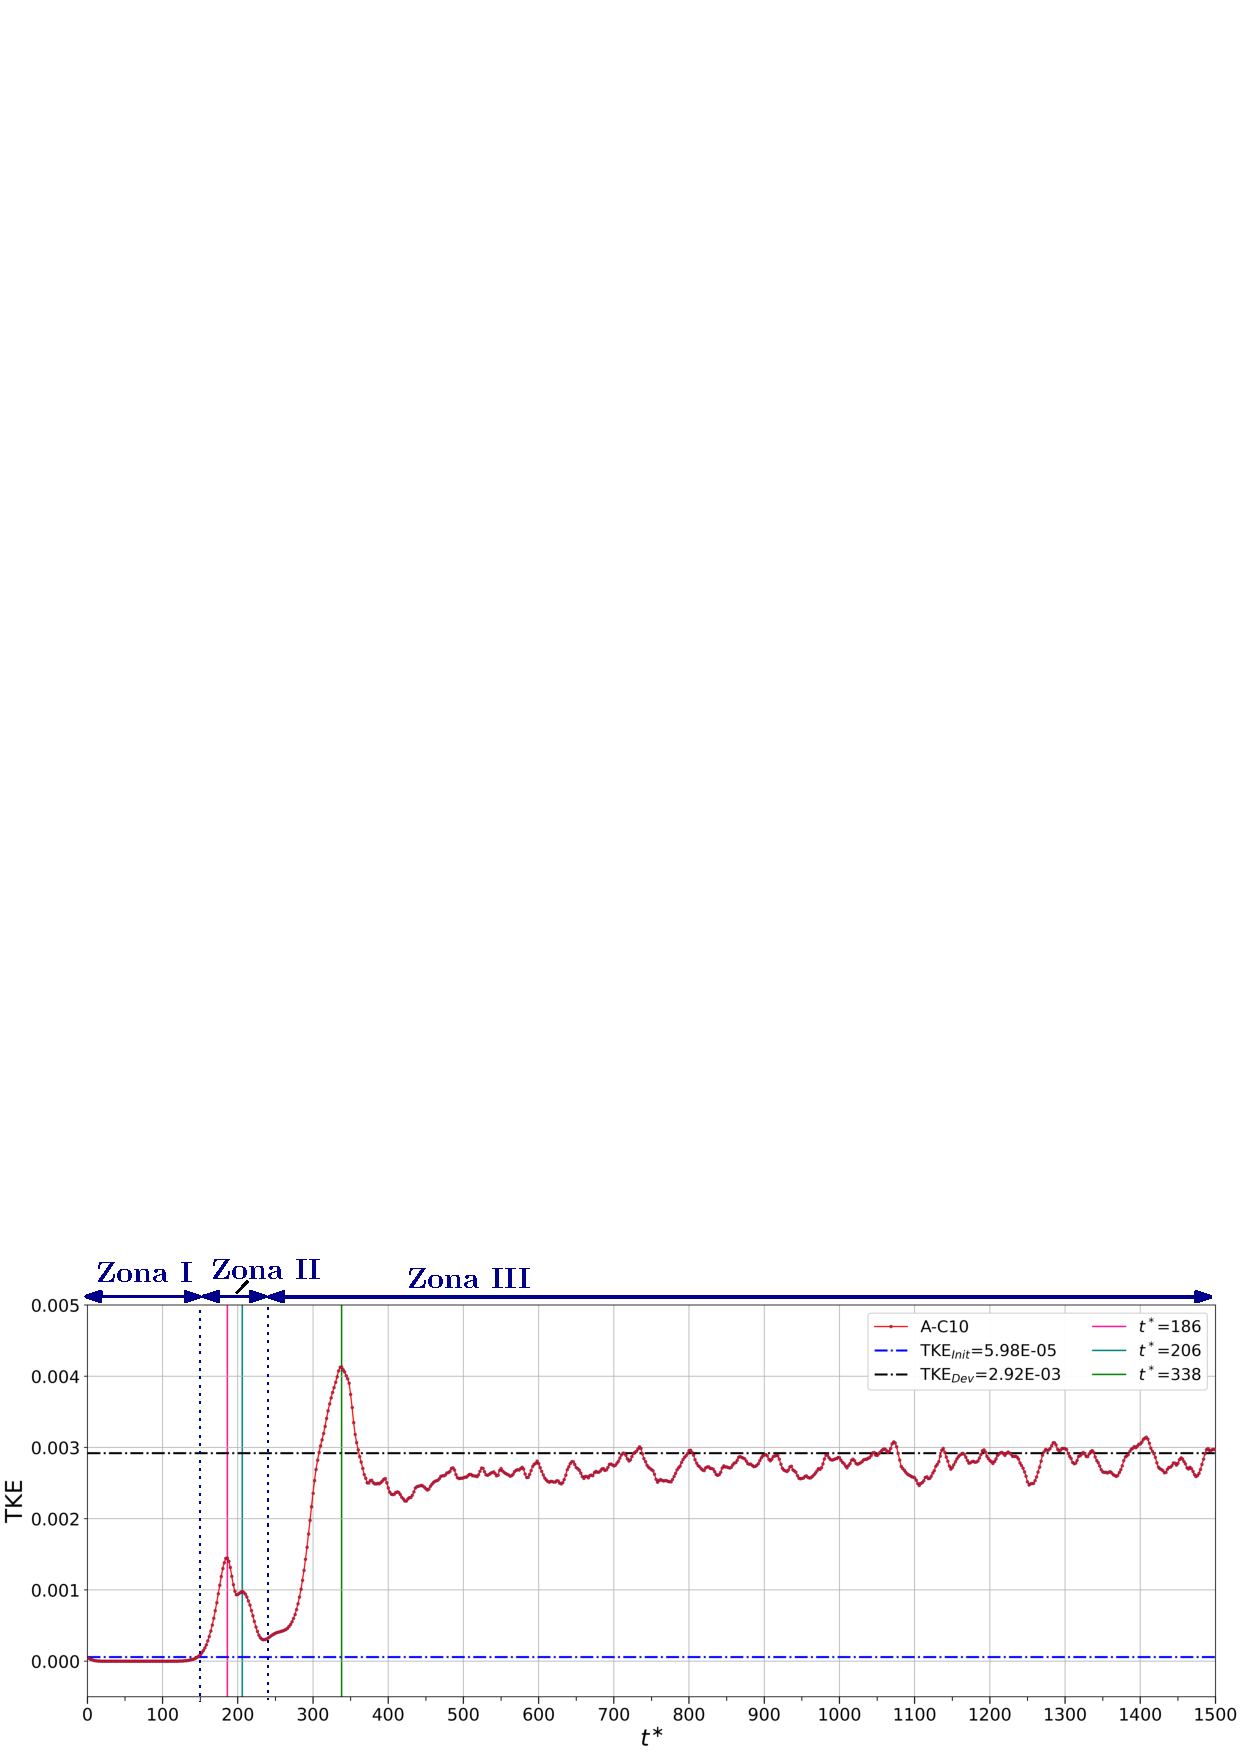
\includegraphics[width=0.49\textwidth]{figures/cap6/Re5000-Pr071-Ri1Em6/Cases_Comp_tke.png}
    \label{fig:tke-Re5000-Pr071}}  
  \subfloat[]{
    \includegraphics[width=0.49\textwidth]{figures/cap6/Re5000-Pr071-Ri1Em6/Cases_Comp_retau.png}
    \label{fig:retau-Re5000-Pr071}}
  \caption{Evolución temporal de \textbf{(a)} TKE y \textbf{(b)} Re$_{\tau}$ para las distintas condiciones iniciales del caso A.}
  \label{fig:case-A-Re5000-Pr071}
\end{figure}



\subsection{Caso B (Ri$_b$=1.06)}

Los parámetros de las perturbaciones utilizadas para la construcción de las condiciones iniciales se resumen en la Tabla \ref{tab:grupo2}. Los ensayos B‑C2 y B‑C3 utilizan únicamente una onda bidimensional ($\text{A}_{\text{2D}}=2 \%$) con diferente autovalor y autofunción, mientras que B‑C4 y B‑C5 añaden una combinación de ondas oblicuas 3D de pequeña amplitud ($\text{A}_{\text{3D}}= 0\text{.}4\%$). En la Figura \ref{fig:case-B-Re5000-Pr071} se expone la evolución en el tiempo de TKE y Re$_{\tau}$ para las distintas condiciones iniciales consideradas.  

En los cuatro ensayos, todas las perturbaciones mencionadas inducen la transición del flujo. Tanto la energía cinética turbulenta como el Re$_{\tau}$ experimentan un crecimiento abrupto en una etapa muy temprana de la transición ($t^*\lesssim 30$). En el caso de Re$_{\tau}$, los máximos se alcanzan para $t^*\lesssim 60$. En particular, en el ensayo B‑C4, el pico se produce casi en la mitad del tiempo ($t^*\approx 25$) que en el resto de los ensayos. Esta cuestión coincide con el hecho de que la parte imaginaria de su autovalor 2D es positiva en comparación al resto de casos que resulta negativa; es decir, se tiene un modo que es más inestable. Luego, para $t^* \gtrsim 150$, el Re$_{\tau}$ se estabiliza en torno a un valor próximo a 270, lo que indica que se ha alcanzado un nuevo estado de flujo. De acuerdo a la línea a trazos (negra) graficada, correspondiente al flujo turbulento del caso completamente desarrollado, se puede afirmar que el flujo transicionó hacia un régimen turbulento.  

Por su parte, la evolución de la TKE comparte ciertos rasgos a los descritos para Re$_{\tau}$. En el ensayo B-C4, el pico se alcanza casi en la mitad del tiempo que en el resto de casos ($t^*\approx 50$); para $t^* \gtrsim 100$, la energía cinética turbulenta se reduce y permanece en torno a un valor constante, $\kappa \approx 0\text{.}002$, que corresponde al caso completamente desarrollado, corroborando también que efectivamente el sistema ha alcanzado un estado de flujo turbulento. Un detalle a destacar es que, mientras en la TKE el máximo alcanzado en el ensayo B-C4 supera al de los demás casos, en el Re$_{\tau}$ ocurre lo contrario: el pico correspondiente al caso B-C4 resulta menor que los picos de los demás ensayos. Se presume que el aumento de la tensión de corte en B-C4 no resulta tan efectivo como en los casos B-C2, B-C3 y B-C5 debido a la gran producción de turbulencia que actúa difundiendo el momento. Por último, para los tiempos adimensionales tales que $t^* > 100$, todas las curvas colapsan, indicando que la dinámica final del sistema, en el estado estadísticamente estacionario, no depende de la perturbación inicial impuesta. 


\paragraph{Caso representativo.} En todos los ensayos del Caso B se logra que el sistema transicione al régimen turbulento. En cada uno se observa un crecimiento, un pico y un decaimiento que tiende al estado turbulento. Se elige el ensayo B‑C2 ya que su transición se alcanza con una perturbación bidimensional  únicamente, a diferencia de lo ocurrido con el caso A.   

\begin{table}[H]
\centering
\caption{Parámetros de las condiciones iniciales para el caso B (Re$_o$ = 5000, Pr = 0.71, Ri$_b$ = 1.06).}
\label{tab:grupo2}
\resizebox{0.75\textwidth}{!}{%
\begin{tabular}{lcccccc}
\toprule
Nomenclatura & $\alpha$ &   $\beta$ &   A$_{2D}$ [\%] &  A$_{3D}$ [\%] & $c_{2D}$ & $c_{3D}$ \\
\midrule
B‑C2 & 1.12 & 0   & 2 & 0   & 0.800 - 0.495 j & - \\
B‑C3 & 1.12 & 0   & 2 & 0   & 2.853 - 0.107 j & - \\
B‑C4 & 1.12 & 2.1 & 2 & 0.4 & 2.315 + 0.424 j & 1.721 + 0.235 j \\
B‑C5 & 1.12 & 2.1 & 2 & 0.4 & 2.853 - 0.107 j & 1.550 + 0.023 j \\
\bottomrule
\end{tabular}}
\end{table}

\begin{figure}[H]
  \centering  
  \subfloat[]{
    \includegraphics[width=0.49\textwidth]{figures/cap6/Re5000-Pr071-Ri1Em4/Cases_Comp_retau.png}
    \label{fig:retau-Re5000-Pr071}}
  \subfloat[]{
    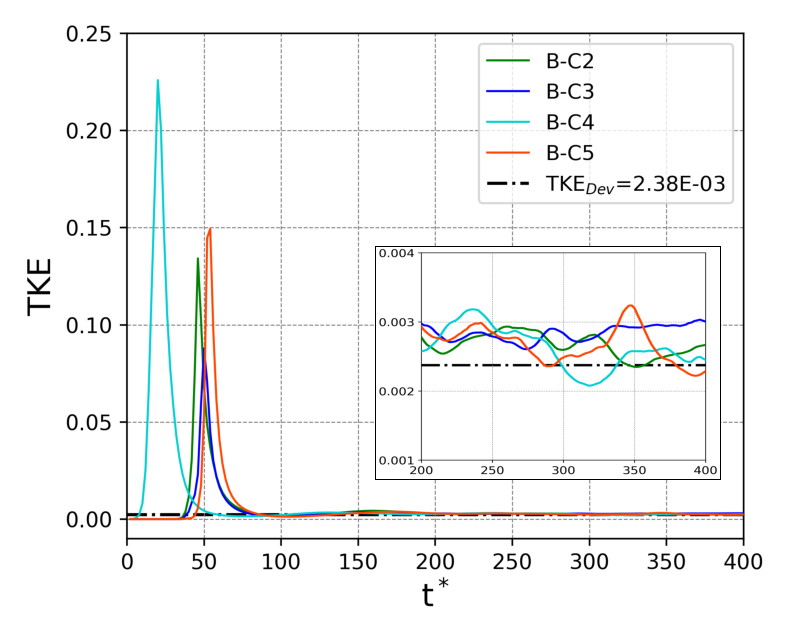
\includegraphics[width=0.49\textwidth]{figures/cap6/Re5000-Pr071-Ri1Em4/Cases_Comp_tke.eps}
    \label{fig:tke-Re5000-Pr071}}

  \caption{Evolución temporal de \textbf{(a)} Re$_{\tau}$ y \textbf{(b)} TKE para las distintas condiciones iniciales del caso B.}
  \label{fig:case-B-Re5000-Pr071}
\end{figure}

\newpage

\section{Análisis detallado del caso A-C10} \label{sec:ac10}

\subsection{TKE y Varianza de la temperatura adimensional}

En las Figuras \ref{fig:tke-ac10} y \ref{fig:tetavar-ac10} la evolución temporal de las magnitudes consideradas (curva roja) se separa en cuatro zonas diferenciadas. A modo de referencia se añaden los valores constantes asociados a la condición inicial y al flujo turbulento completamente desarrollado.

\begin{itemize}
\item \textbf{Zona I (0 $\lesssim$ $\mathbf{t^*}$ $\lesssim$ 150).} Ambas magnitudes experimentan un leve descenso al inicio, luego permanecen prácticamente constantes, sin incrementos ni descensos, y posteriormente aumentan hasta recuperar sus valores iniciales. En este tramo, ambas magnitudes permanecen por debajo de los valores completamente desarrollados del caso turbulento correspondiente. En este intervalo las perturbaciones iniciales no modifican significativamente el flujo base.

\item \textbf{Zona II (150 $\lesssim$ $\mathbf{t^*}$ $\lesssim$ 234)}. La energía cinética turbulenta presenta dos máximos locales bien definidos en torno a $t^*\approx186$ y $t^*\approx206$, separados por un valle intermedio. Por su parte, la varianza de la temperatura experimenta una evolución similar en el mismo intervalo temporal: crece tres órdenes de magnitud, presenta un máximo local, desciende hasta un valle y crece hasta un segundo máximo de menor intensidad. Luego, ambas magnitudes descienden parcialmente antes de volver a crecer.

\item \textbf{Zona III (234 $\lesssim$ $\mathbf{t^*}$ $\lesssim$ 338).} Tanto la TKE, como $\langle \theta^{* \prime} \theta^{* \prime} \rangle$ crecen de forma sostenida, con un cambio de pendiente que ocurre alrededor de $t^*\approx276$. Luego, la TKE alcanza un máximo absoluto en torno a $t^*\approx338$ ($\kappa_{max} \approx 4\text{.}1 \times 10^{-3}$) y la varianza alcanza su máximo absoluto cerca de $t^*\approx320$ con un valor alrededor de $\langle \theta^{* \prime} \theta^{* \prime} \rangle_{\text{max}} \approx 2 \times 10^{4}$. En este intervalo se observa la influencia de la perturbación 3D, que produce un nuevo crecimiento descripto conceptualmente por la inestabilidad secundaria.

\item \textbf{Zona IV ($\mathbf{t^*} \gtrsim 338$).} En una primera etapa, la energía cinética turbulenta desciende desde su valor máximo hasta quedar por debajo del valor constante del caso turbulento completamente desarrollado; posteriormente, aumenta y fluctúa en torno a dicho valor, dentro del rango $\left[ 2\text{.}5 \text{ , } 3\text{.}5 \right] \times 10^{-3}$. Por su parte, la varianza de la temperatura desciende de manera gradual, acercándose al valor de referencia del caso turbulento desarrollado.
\end{itemize}

\newpage

\begin{figure}[H]
  \centering  
  \subfloat[]{
    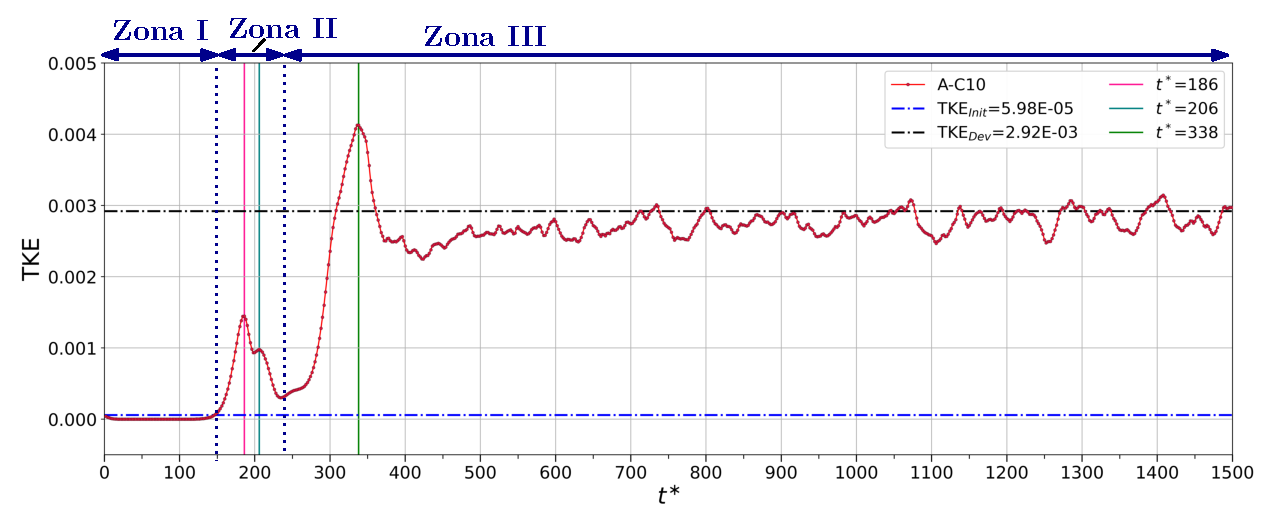
\includegraphics[width=0.9\textwidth]{figures/cap6/A-C10/Cases_Comp_tke.eps}
    \label{fig:tke-ac10}}
    
  \subfloat[]{
    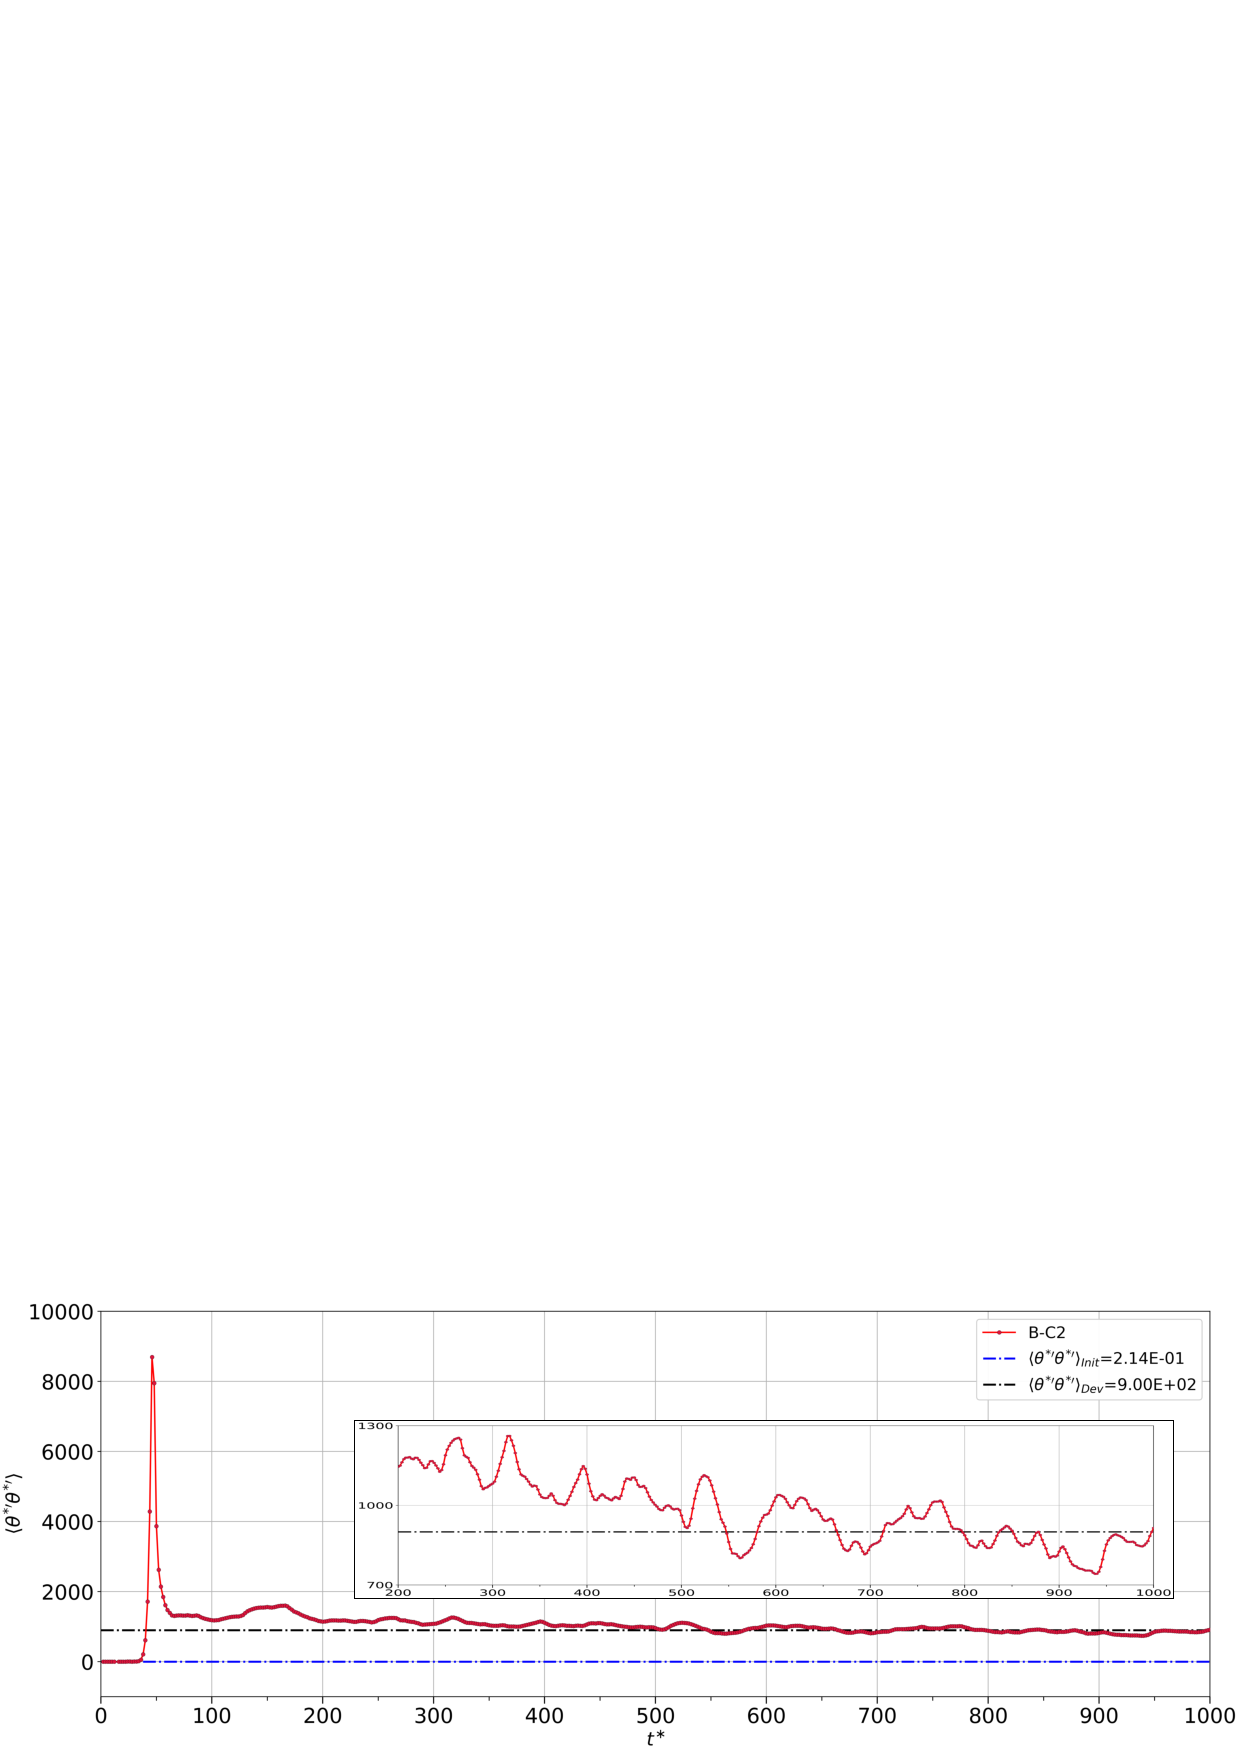
\includegraphics[width=0.9\textwidth]{figures/cap6/A-C10/Cases_Comp_tetavar.png}
    \label{fig:tetavar-ac10}}
  \caption{Evolución temporal de \textbf{(a)} la energía cinética turbulenta y \textbf{(b)} la varianza de la temperatura, para el caso A-C10.}
  \label{fig:ac10-2}
\end{figure}

\subsection{Perfiles de velocidad y temperatura}

En las Figuras \ref{fig:uxs-ac10} y \ref{fig:phis-ac10} se muestran, respectivamente, los perfiles de velocidad y \linebreak temperatura adimensional para $t^*=2$, $186$, $206$, $338$, $750$, $1500$ (de izquierda a derecha). A modo de referencia, se incluye el perfil correspondiente al flujo turbulento completamente \linebreak desarrollado. Los instantes elegidos abarcan la etapa laminar inicial ($t^*=2$), los máximos locales ($t^* \approx 186$ y $t^* \approx 206$), el máximo absoluto de la TKE y dos tiempos en los que el flujo ya es turbulento.

La perturbación impuesta modifica el perfil de velocidad que en un inicio tiene forma de ``M'' (véase Sección \ref{sec:mix-laminar}). A medida que el flujo evoluciona se observa que en $t^* \approx 186$ y $t^* \approx 206$, los perfiles conservan la simetría pero no mantienen su forma característica inicial. Esta forma relativamente más plana en los perfiles es consecuencia de un aumento de la difusión de momento dada por el incremento de turbulencia (véase Figura \ref{fig:tke-ac10}). Asimismo, próximo a $t^* \approx 338$, se aprecia una aparente ``pérdida'' en la simetría del perfil. En una etapa ya turbulenta, los perfiles de velocidad se aproximan a aquel correspondiente al flujo completamente desarrollado. Los perfiles de temperatura adimensional siguen una evolución análoga: se deforman manteniendo su simetría, luego la misma se desvanece momentáneamente en $t^* \approx 338$ (el perfil se vuelve asimétrico), y posteriormente tienden hacia el perfil del caso turbulento desarrollado. El efecto de la turbulencia aplana los perfiles de temperatura y aproxima la temperatura en el centro del canal al valor de aquella impuesta en la pared. Por otro lado, al inspeccionar los perfiles de velocidad y temperatura en conjunto, se observa que el desarrollo de la parte hidrodinámica se encuentra ligeramente acelerado respecto al desarrollo térmico. Este hecho depende del número de Prandtl (Pr) y de cuán relevante es la boyancia en la ecuación de momento (Ri$_b$).


\begin{figure}[H]
  \centering  
  \subfloat[]{
    \includegraphics[width=1.05\textwidth]{figures/cap6/A-C10/ux_profiles_mosaic.png}
    \label{fig:uxs-ac10}}
  
  \subfloat[]{
    \includegraphics[width=1.05\textwidth]{figures/cap6/A-C10/phi_profiles_mosaic.png}
    \label{fig:phis-ac10}}
  \caption{Perfiles de \textbf{(a)} velocidad y \textbf{(b)} temperatura adimensional para distintos instantes $t^*$ correspondientes al caso A-C10.}
  \label{fig:mosaico-ac10}
\end{figure} 

Respecto a la pérdida momentánea de simetría mostrada en los perfiles de la Figura \ref{fig:mosaico-ac10}  se especula que se debe a un efecto de dominio. Un dominio que abarque más de una longitud de onda de las perturbaciones iniciales, en las direcciones $X$ y $Z$, podría compensar este efecto. %Por cuestiones de costo computacional la verificación de esta hipótesis queda para estudios futuros.

Con el fin de profundizar en el entendimiento de la aparente pérdida de simetría observada en los perfiles para el instante $t^* = 338$, resulta ilustrativo examinar las estructuras de vórtices del flujo. Dichas estructuras se obtienen mediante el ``Criterio Q'' \cite{hunt1988eddies}. El análisis que se realiza a continuación se hace con un enfoque cualitativo. En la Figura \ref{fig:mosaico2-ac10} se exponen capturas de las ``isosuperficies de Q'' para tres tiempos distintos: $t^* = 186$ (Figuras \ref{fig:t186-xy-ac10} y  \ref{fig:t186-zy-ac10}),  $t^* = 338$  (Figuras \ref{fig:t338-xy-ac10} y  \ref{fig:t338-zy-ac10}) y  $t^* = 1500$  (Figuras \ref{fig:t1500-xy-ac10} y  \ref{fig:t1500-zy-ac10}); las capturas ubicadas a la derecha corresponden a la vista del dominio desde un punto de vista normal a los planos $ZY$, mientras que las ubicadas a la izquierda muestran la vista normal a los planos $XY$.

En el instante $t^* = 186$, se observa una estructura coherente y ordenada, asociada a las ondas TS; esto es consistente con el hecho de que los perfiles en la condición inicial tengan una simetría respecto a la dirección $Y$ (antes de que ocurra el máximo absoluto de la TKE). 

\newpage

En el segundo instante considerado (Figuras \ref{fig:t338-xy-ac10} y \ref{fig:t338-zy-ac10}), las capturas revelan una mayor presencia de estructuras de vórtices en la pared superior ($\text{y}=2$) respecto a la inferior ($\text{y}=0$); esto último se puede corroborar mirando capturas adicionales en las Figuras \ref{fig:t338-v1-ac10} y \ref{fig:t338-v2-ac10} que muestran el dominio desde otros puntos de vista. Este ``desbalance'' de estructuras da sustento a la idea supuesta de ``pérdida en la simetría'' de los perfiles de velocidad y temperatura antes mencionada. Nótese (Figura \ref{fig:t338-zy-ac10}), que si bien las estructuras ya no son simétricas respecto al plano $ZX$\footnote{En esta captura, la posición de este plano se encuentra en Y=1.} en $y^*=0$ (representado por la línea azul) se puede apreciar cierta simetría respecto al plano $XY$\footnote{En esta captura, la posición de este plano se encuentra en Z=1.5.} en $z^*= 1 \text{.} 5$ (señalado por la línea roja). En este sentido, todavía se puede considerar que, en $t^* = 338$, el flujo conserva cierto grado de orden y coherencia. 


En el último instante, donde el flujo ya se ha desarrollado y se encuentra en estado estadísticamente estacionario, las estructuras han dejado de ser coherentes y tienden a organizarse cerca de las paredes, en consistencia con los perfiles simétricos característicos de los flujos turbulentos completamente desarrollados \cite{machaca2024}.

\begin{figure}%[H]
  \centering  
  \subfloat[]{
    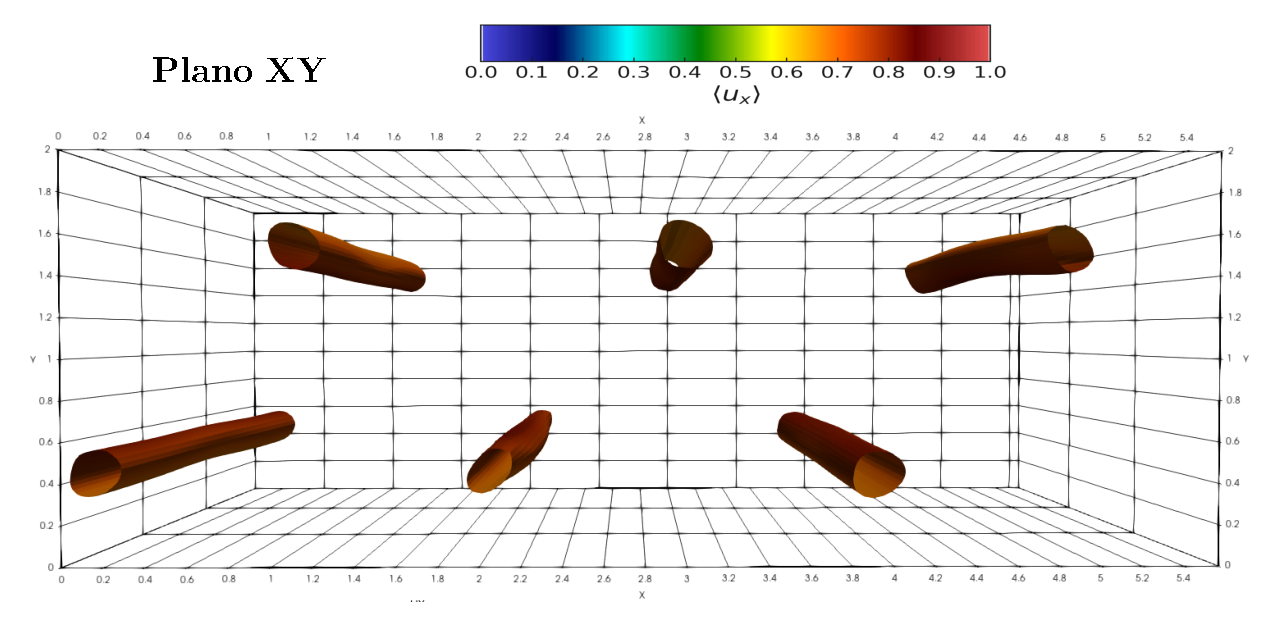
\includegraphics[width=0.58\textwidth]{figures/cap6/A-C10/screenshots_times/t186_xy.eps}
    \label{fig:t186-xy-ac10}}  
  \subfloat[]{
    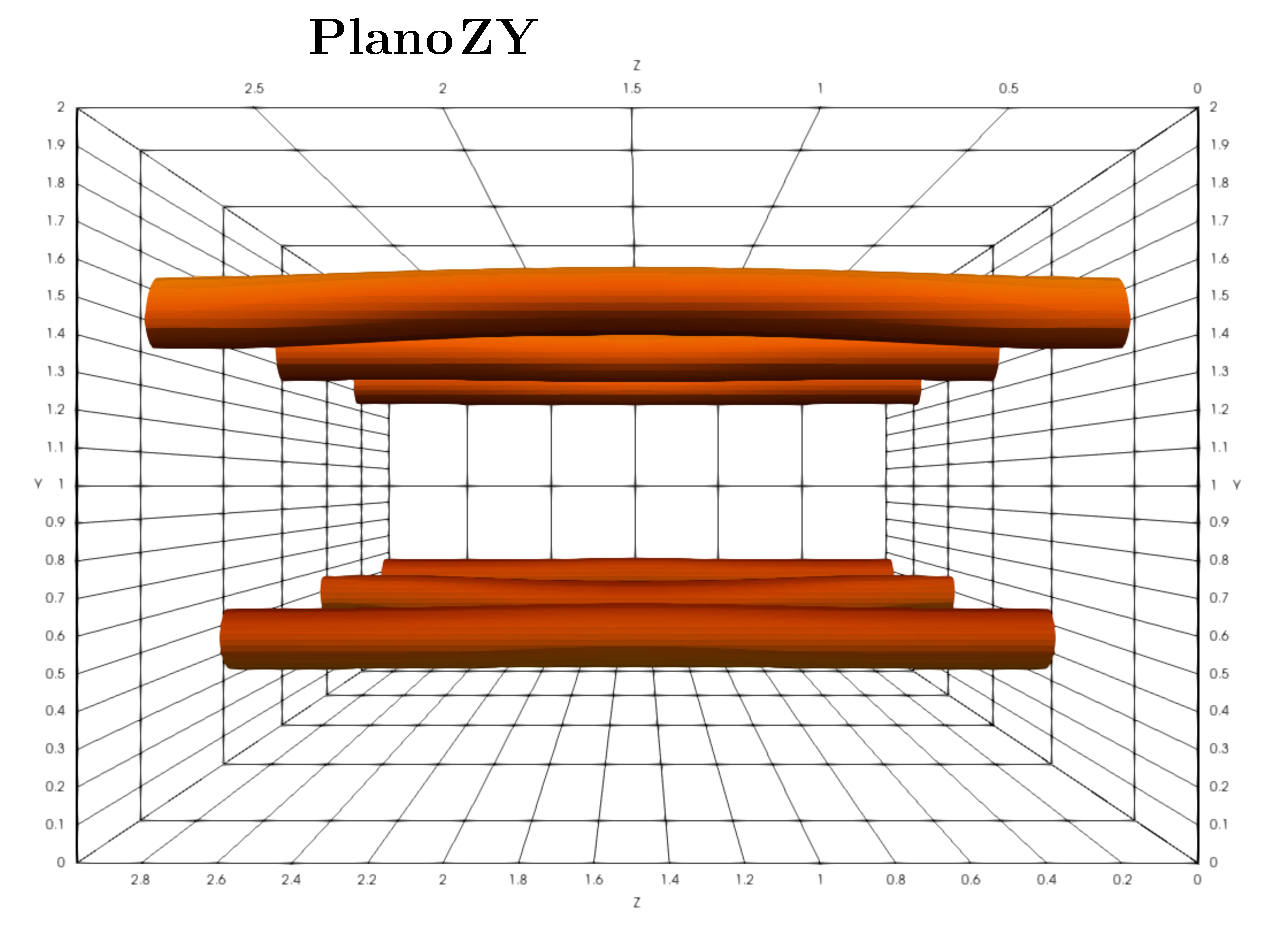
\includegraphics[width=0.40\textwidth]{figures/cap6/A-C10/screenshots_times/t186_zy.eps}
    \label{fig:t186-zy-ac10}}
    
  \subfloat[]{  
    \includegraphics[width=0.58\textwidth]{figures/cap6/A-C10/screenshots_times/t338_xy.png}
    \label{fig:t338-xy-ac10}}  
  \subfloat[]{
    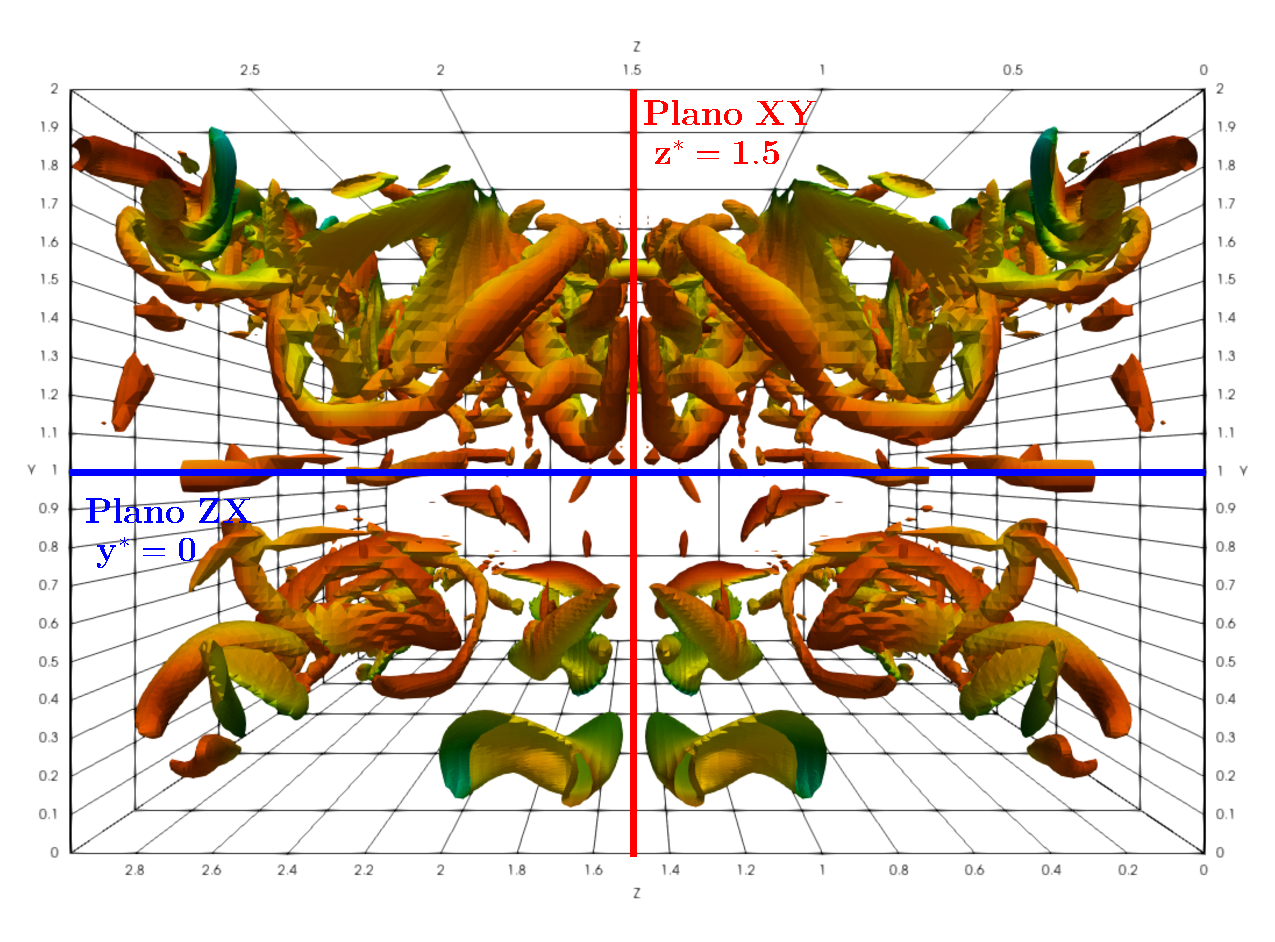
\includegraphics[width=0.40\textwidth]{figures/cap6/A-C10/screenshots_times/t338_zy.eps}
    \label{fig:t338-zy-ac10}}
  
  \subfloat[]{ 
    \includegraphics[width=0.58\textwidth]{figures/cap6/A-C10/screenshots_times/t1500_xy.png}
    \label{fig:t1500-xy-ac10}}  
  \subfloat[]{
    \includegraphics[width=0.40\textwidth]{figures/cap6/A-C10/screenshots_times/t1500_zy.png}
    \label{fig:t1500-zy-ac10}}
  \caption{Ensayo A-C10. Capturas de las estructuras de vórtices para tres instantes de tiempo: $t^* =186$ con $Q=0\text{.}1$ (\textbf{(a)} y \textbf{(b)}), $t^* =338$ con $Q=0\text{.}5$ (\textbf{(c)} y \textbf{(d)}) y $t^* = 1500$ con $Q=0\text{.}5$ (\textbf{(e)} y \textbf{(f)}). Aquí $Q$ hace referencia al parámetro del Criterio Q. \textit{Observación: la escala de colores de la captura en \textbf{(a)} se aplica al resto de figuras}.}
  \label{fig:mosaico2-ac10}
\end{figure}

\begin{figure}%[H]
  \centering  
  \subfloat[]{
    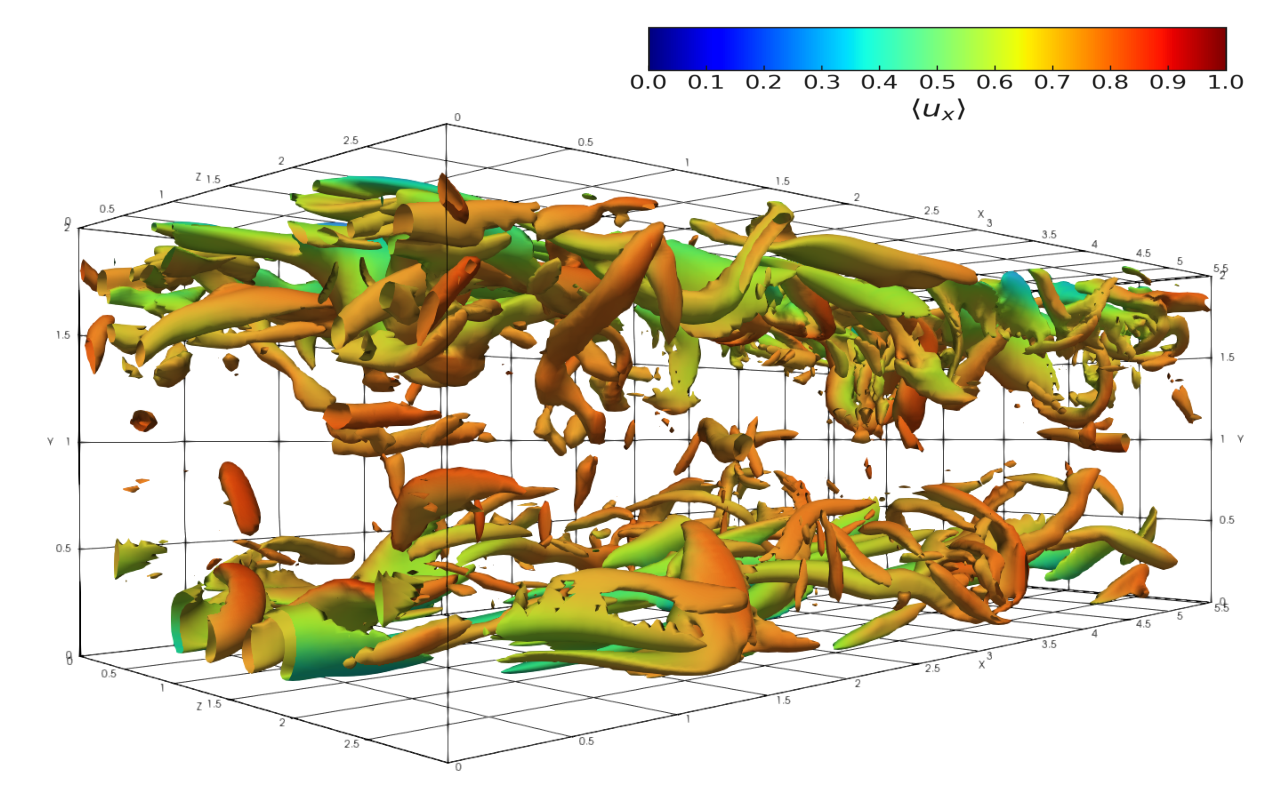
\includegraphics[width=0.49\textwidth]{figures/cap6/A-C10/screenshots_times/t338_v1.eps}
    \label{fig:t338-v1-ac10}}
  \subfloat[]{
    \includegraphics[width=0.49\textwidth]{figures/cap6/A-C10/screenshots_times/t338_v2.png}
    \label{fig:t338-v2-ac10}}
  \caption{Capturas adicionales de las estructuras de vórtices para $t^* =338$ desde otros puntos de vista ($Q=0\text{.}5$).}
  \label{fig:mosaico-ac10-v1-v2}
\end{figure}

\subsection{Factor de fricción de Darcy y número de Nusselt}
En la Figura \ref{fig:darcy-ac10} se presenta la evolución temporal del factor de fricción de Darcy. En la \textbf{Zona I} ($0 < t^* < 150$), $f$ permanece prácticamente constante y coincide con el \linebreak valor inicial/laminar\footnote{Recuérdese que los valores de $f$ y Nu obtenidos a partir de la solución laminar y de la condición inicial resultan equivalentes.} (línea a trazos azul). En las \textbf{Zonas II} y \textbf{III}, y parte de la \textbf{Zona IV} ($150 \lesssim t^* \lesssim 352 $), se observa primero una disminución suave hasta un mínimo de $f=0\text{.}0167$ en $t^*\approx270$, seguida de un incremento pronunciado que alcanza su máximo en $t^*\approx352$ ($f \approx 0\text{.}037$). A partir de ese pico, y en el resto de la \textbf{Zona IV} ( $t^*\gtrsim352$), $f$ desciende y se estabiliza entre los valores 0.0275 y 0.033, en torno al valor de referencia del caso completamente desarrollado (línea a trazos negra). De esta forma, es posible distinguir con claridad la etapa transitoria y el posterior establecimiento de un régimen turbulento que persiste en el tiempo.

Por último, la Figura \ref{fig:nu-ac10} presenta la evolución temporal del número de Nusselt. El valor se mantiene prácticamente constante y coincidente con la solución laminar hasta $t^* \approx 300$. A partir de allí, crece de manera monótona hasta el final de la simulación. La magnitud tiende al valor correspondiente al régimen turbulento desarrollado (convección mixta); sin embargo, el tiempo físico simulado no resulta suficiente para garantizar la convergencia. Esta misma situación puede observarse en la varianza de la temperatura y en el perfil de temperatura para $t^*=1500$ aunque no de manera tan marcada como en el caso de Nu. Esto sugiere que se requiere extender la simulación para que las magnitudes térmicas alcancen su estado estadísticamente estacionario.

\begin{figure}[H]
  \centering  
  \subfloat[]{
    \includegraphics[width=0.9\textwidth]{figures/cap6/A-C10/Cases_Comp_darcy.png}
    \label{fig:darcy-ac10}}
    
  \subfloat[]{
    \includegraphics[width=0.9\textwidth]{figures/cap6/A-C10/Cases_Comp_nussel.png}
    \label{fig:nu-ac10}}
  \caption{Evolución temporal de \textbf{(a)} factor de fricción de Darcy y \textbf{(b)} número de Nusselt, para el caso A-C10.}
  \label{fig:ac10-1}
\end{figure}



\newpage
\section{Análisis detallado del caso B‑C2} \label{sec:bc2}

\subsection{TKE y varianza de la temperatura adimensional}
En las Figuras \ref{fig:tke-bc2} y \ref{fig:tetavar-bc2} se expone, respectivamente, la evolución temporal de la energía cinética turbulenta (TKE) y la varianza de la temperatura; dicha evolución se separa en tres regiones. Se añaden valores constantes de referencia asociados al cálculo de dichas cantidades empleando la condición inicial y el flujo turbulento en estado estadísticamente estacionario.

\begin{itemize}

  \item \textbf{Zona I ($0 \lesssim \mathbf{t^*} \lesssim 32$).} Ambas cantidades se mantienen prácticamente constantes y coinciden con su valor de referencia asociado a la condición inicial. El sistema no transiciona.

  \item \textbf{Zona II ($32 \lesssim \mathbf{t^*} \lesssim 100$).} Aquí, la TKE crece y alcanza un máximo absoluto en $t^* \approx 46$ ($\kappa_{\text{max}}$ $\approx 0\text{.}134$). De forma similar, la varianza de la temperatura crece hasta que alcanza un máximo absoluto en el mismo instante de tiempo que la TKE, con un valor $\langle \theta^{*\prime} \theta^{*\prime}\rangle_{\text{max}} \approx 8700$. A partir de $t^* \approx 46$, ambas magnitudes decrecen sin retornar a los valores iniciales, y tienden hacia el estado estadísticamente estacionario del flujo turbulento correspondiente.

% NO BORRAR
%  \item \textbf{Zona II ($32 \lesssim \mathbf{t^*} \lesssim 100$).} Aquí, la TKE crece y alcanza un máximo absoluto en $t^* \approx 46$ ($k_{\text{max}}$ $\approx 0\text{.}134$), superando en dos órdenes de magnitud al valor registrado en el ensayo A-C10. De forma similar, la varianza de la temperatura crece hasta que alcanza un máximo absoluto en el mismo instante de tiempo que la TKE, con un valor $\langle \theta^{*\prime} \theta^{*\prime}\rangle_{\text{max}} \approx 8700$, siendo casi un orden de magnitud menor que en el ensayo A-C10. A partir de $t^* \approx 46$, ambas magnitudes decrecen sin retornar a los valores iniciales, y tienden hacia el estado estadísticamente estacionario del flujo turbulento correspondiente.

  \item \textbf{Zona III ($\mathbf{t^*} \gtrsim 100$).} En esta etapa, ambas magnitudes experimentan un segundo máximo local, de mucha menor intensidad, en $t^* \approx 160$. Luego, para $t^* > 200$, ambas cantidades fluctúan en torno a las magnitudes constantes de referencia: la TKE se mantiene acotada entre 0.002 y 0.003, mientras que la varianza de la temperatura se encuentra entre 700 y 1300. Para $t^* >200$, el sistema tiende hacia un nuevo estado de flujo, es decir, uno turbulento. 

\end{itemize}


\begin{figure}[H]
  \centering  
    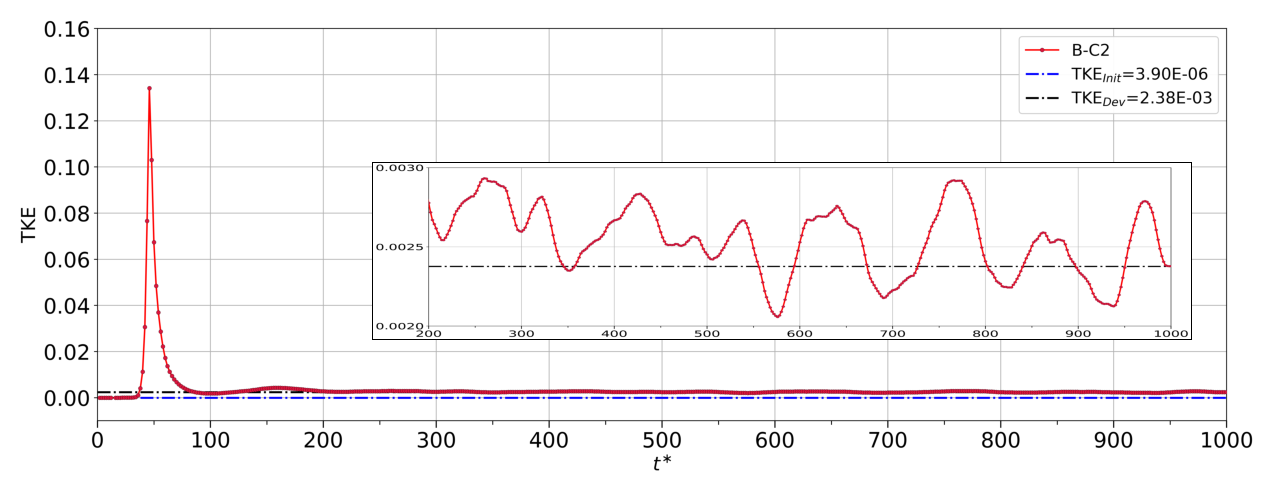
\includegraphics[width=0.9\textwidth]{figures/cap6/B-C2/Cases_Comp_tke.eps}
   \caption{Evolución temporal de la energía cinética turbulenta para el caso B-C2.}
    \label{fig:tke-bc2}
\end{figure}

\newpage

\begin{figure}[H]
  \centering      
    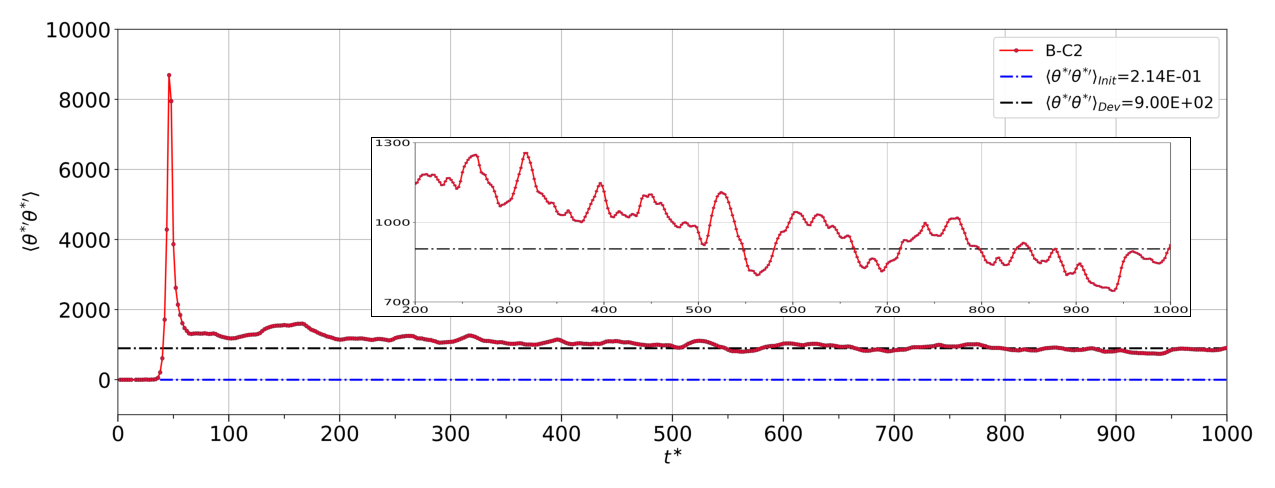
\includegraphics[width=0.9\textwidth]{figures/cap6/B-C2/Cases_Comp_tetavar.eps}
     \caption{Evolución temporal de la varianza de la temperatura para el caso B-C2.}
      \label{fig:tetavar-bc2}
\end{figure}

\subsection{Perfiles de velocidad y temperatura}
En las Figuras \ref{fig:uxs-bc2} y \ref{fig:phis-bc2} se presentan, respectivamente, los perfiles de velocidad y de temperatura adimensional para $t^*$ = 2, 46, 160, 500, 1000 (de izquierda a derecha). Como referencia, se incluye el perfil correspondiente al flujo completamente desarrollado en convección mixta. La selección de tiempos abarca el régimen laminar inicial ($t^* = 2$), el máximo absoluto en $t^* \simeq 46$, el máximo local subsiguiente de mucha menor intensidad, en $t^* \simeq 160$, y dos instantes posteriores en los que el flujo ya se encuentra en régimen turbulento.

En la etapa inicial, el perfil exhibe la simetría característica de la solución laminar en forma de ``M''. En torno al máximo absoluto de la TKE, los perfiles se ensanchan levemente y muestran, nuevamente, una aparente pérdida de simetría. A medida que aumenta el tiempo adimensional, los perfiles de ambas magnitudes convergen hacia las soluciones de referencia del flujo completamente desarrollado. Al compararse con el ensayo A-C10 (Figura \ref{fig:phis-ac10}), se observa que el aumento de la fuerza boyante tiene por efecto acelerar la evolución del campo de temperaturas, favoreciendo una convergencia más rápida hacia el flujo completamente desarrollado.


Nuevamente, se analizan las estructuras de vórtices mediante un enfoque cualitativo, con la intención de entender la aparente pérdida de simetría en los perfiles que ocurre a $t^* = 46$. En la Figura \ref{fig:mosaico2-bc2} se exponen capturas de las isosuperficies de Q asociadas a tres tiempos distintos: $t^* = 2$ (Figuras \ref{fig:t2-xy-bc2} y  \ref{fig:t2-zy-bc2}),  $t^* = 46$  (Figuras \ref{fig:t46-xy-bc2} y \ref{fig:t46-zy-bc2}) y  $t^* = 500$  (Figuras \ref{fig:t500-xy-bc2} y \ref{fig:t500-zy-bc2}). Obsérvese que las capturas ubicadas a la derecha corresponden a la vista del dominio desde un punto de vista normal a los planos $ZY$, mientras que las ubicadas a la izquierda muestran la vista normal a los planos $XY$.

\newpage

\begin{figure}[H]
  \centering  
  \subfloat[]{
    \includegraphics[width=1.02\textwidth]{figures/cap6/B-C2/ux_profiles_mosaic.png}
    \label{fig:uxs-bc2}}
  
  \subfloat[]{
    \includegraphics[width=1.02\textwidth]{figures/cap6/B-C2/phi_profiles_mosaic.png}
    \label{fig:phis-bc2}}
  \caption{Perfiles de \textbf{(a)} velocidad y \textbf{(b)} temperatura adimensional para distintos instantes $t^*$ correspondiente al caso B-C2.}
    \label{fig:mosaico-bc2}
\end{figure}




En el instante $t^* = 2$, se observa una estructura coherente y ordenada, asociada a las ondas TS. Esto es consistente con la simetría de los que perfiles en la condición inicial; asimismo, dichas estructuras se posicionan muy cerca de las paredes al igual que ocurre con los máximos del perfil de velocidad.

En el segundo instante de tiempo considerado, se observa que las estructuras no se \linebreak aglomeran de forma simétrica respecto a las paredes ($y^*=\pm 1$). Una visualización más clara, se aprecia en las Figuras \ref{fig:t46-zy_x1}-\ref{fig:t46-zy_x5} donde se muestran cortes de planos $ZY$ para $x^*=1,2,4,5$, respectivamente. A partir de estos cortes se observa que, a lo largo de la dirección $X$, las estructuras se distribuyen de manera no uniforme cerca de las paredes. Este ``desequilibrio'' de pequeñas estructuras produce una mezcla no homogénea de las cantidades, lo que podría dar cierto entendimiento, al menos conceptual, del hecho que los máximo del perfil de velocidad cerca las paredes sea levemente distinto en el dominio simulado.   

Por su parte, en el último instante de tiempo considerado (estado estadísticamente estacionario), se aprecia que las estructuras  tienden a aglomerarse cerca de las paredes y también carecen de coherencia y orden (véase Figuras \ref{fig:t500-xy-bc2} y \ref{fig:t500-zy-bc2}). Entonces, dado que la dinámica en ambas paredes es la misma en términos estadísticos, las cantidades de interés resultan, en promedio, simétricas respecto a la dirección $Y$. Esto es consistente con lo observado en el perfil de velocidad \textit{streamwise} (Figura \ref{fig:uxs-bc2} a $t^*=500$).

Resulta evidente que el efecto de la fuerza boyante impacta considerablemente en cómo el fluido evoluciona en el tiempo. Uno de los efectos más notables, como se menciona anteriormente, es la aceleración de la dinámica del sistema. 

\begin{figure} [H]
  \centering  
  \subfloat[]{
    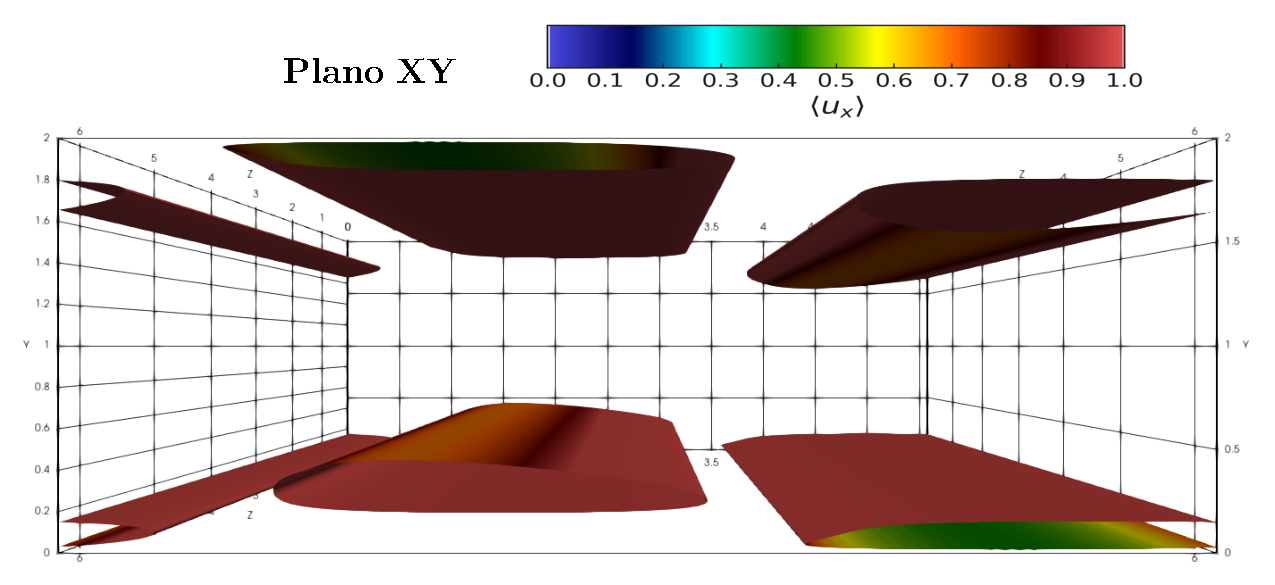
\includegraphics[width=0.48\textwidth]{figures/cap6/B-C2/screenshots_times/t2_xy.eps}
    \label{fig:t2-xy-bc2}}  
  \subfloat[]{
    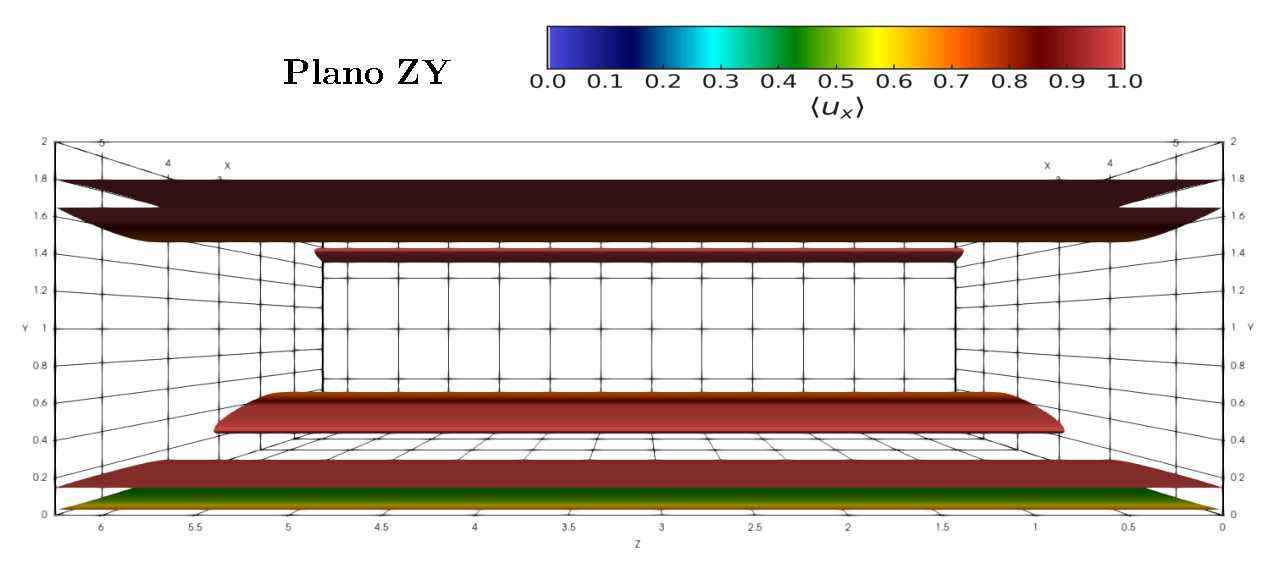
\includegraphics[width=0.5\textwidth]{figures/cap6/B-C2/screenshots_times/t2_zy.eps}
    \label{fig:t2-zy-bc2}}
    
  \subfloat[]{
    \includegraphics[width=0.47\textwidth]{figures/cap6/B-C2/screenshots_times/t46_xy.png}
    \label{fig:t46-xy-bc2}}  
  \subfloat[]{
    \includegraphics[width=0.51\textwidth]{figures/cap6/B-C2/screenshots_times/t46_zy.png}
    \label{fig:t46-zy-bc2}}

  
  \subfloat[]{
    \includegraphics[width=0.47\textwidth]{figures/cap6/B-C2/screenshots_times/t500_xy.png}
    \label{fig:t500-xy-bc2}}  
  \subfloat[]{
    \includegraphics[width=0.51\textwidth]{figures/cap6/B-C2/screenshots_times/t500_zy.png}
    \label{fig:t500-zy-bc2}}
  \caption{Ensayo B-C2. Capturas de las estructuras de vórtices para tres instantes de tiempo: $t^* =2$ con $Q=0\text{.}0005$ (\textbf{(a)} y \textbf{(b)}), $t^* =46$ con $Q=10$ (\textbf{(c)} y \textbf{(d)}) y $t^* = 500$ con $Q=0\text{.}4$ (\textbf{(e)} y \textbf{(f)}). Aquí $Q$ también hace referencia al parámetro del Criterio Q. }
  \label{fig:mosaico2-bc2}
\end{figure}






\subsection{Factor de fricción de Darcy y número de Nusselt}
La Figura \ref{fig:darcy-bc2} muestra la evolución temporal del factor de fricción de Darcy. En las \textbf{Zonas I y II} ($0 \lesssim t^* \lesssim 100$), desde el inicio hasta $t^* \approx 20$, $f$ se mantiene próximo al valor laminar (línea a trazos azul). Entre $t^* \approx 20$ y $t^* \approx 46$ el factor de fricción experimenta dos picos sucesivos antes de culminar en un máximo absoluto de mucho mayor amplitud \linebreak ($f_{\max}$ $\approx$ 0.174). A partir de ese punto, $f$ decrece de manera pronunciada por debajo del valor \linebreak laminar inicial. En la \textbf{Zona III} ($t^* \gtrsim 100$), la curva permanece en torno al valor de la referencia del flujo completamente desarrollado hasta $t^* \approx 400$; luego, la magnitud adquiere valores levemente por debajo del valor de referencia antes mencionado. Esto último es debido a que el sistema necesita más tiempo para desarrollarse. Este efecto se ve más claramente en la siguiente discusión.

La Figura \ref{fig:nu-bc2} muestra la evolución temporal de Nu. Se observa que el número de Nusselt se mantiene cercano a la solución laminar inicial hasta $t^* \approx 34$, luego comienza a decrecer rápidamente hasta un valor mínimo en $t^* \approx 48$ ($\text{Nu}_{\text{min}} \simeq 10\text{.}6$). A partir de allí, Nu comienza un período de crecimiento de manera monótona y sostenida, superando el valor inicial de referencia, tendiendo a la referencia del estado turbulento estadísticamente estacionario. 

\newpage

\begin{figure}[H]
  \centering  
  \subfloat[]{
    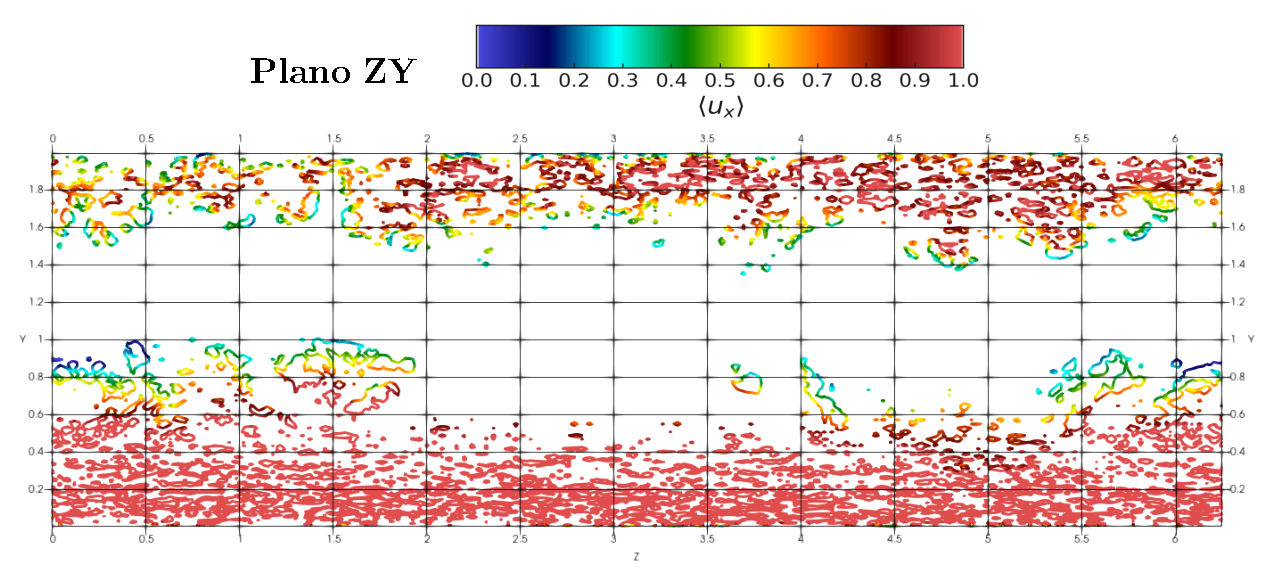
\includegraphics[width=0.49\textwidth]{figures/cap6/B-C2/screenshots_times/zy_x1.eps}
    \label{fig:t46-zy_x1}}  
  \subfloat[]{
    \includegraphics[width=0.49\textwidth]{figures/cap6/B-C2/screenshots_times/zy_x2.png}
    \label{fig:t46-zy_x2}}

  \subfloat[]{
    \includegraphics[width=0.49\textwidth]{figures/cap6/B-C2/screenshots_times/zy_x4.png}
    \label{fig:t46-zy_x4}}  
  \subfloat[]{
    \includegraphics[width=0.49\textwidth]{figures/cap6/B-C2/screenshots_times/zy_x5.png}
    \label{fig:t46-zy_x5}}
    
  \caption{Ensayo B-C2. Cortes de las isosuperficies correspondientes al instante $t^* =46$. Planos $ZY$ para: \textbf{(a)} $x^*=1$, \textbf{(b)} $x^*=2$, \textbf{(c)} $x^*=4$ y \textbf{(d)} $x^*=5$.}
  \label{fig:mosaico3-bc2}
\end{figure}



El valor mínimo que alcanza Nu, coincide aproximadamente con el instante donde TKE es máximo y donde se aprecia, en la Figura \ref{fig:mosaico-bc2}, a $t^*=46$, una gran variación en el perfil de velocidad respecto al correspondiente a $t^*=2$. La TKE ha sido efectiva achatando el perfil de velocidad. Por otro lado, entre estos dos instantes de tiempo, el perfil de temperatura no ha cambiado significativamente, evidenciando un retardo en la evolución del campo de \linebreak temperaturas respecto al observado en la velocidad \textit{streamwise}. Matemáticamente, se aprecia que la temperatura \textit{bulk} (ecuación \ref{eq:tita_bulk}) aumenta entre $t^*=2$ y $t^*=46$ ya que el perfil de velocidad deja de tener peso en los bordes, donde la temperatura es baja, y toma más relevancia en el centro del canal, donde la temperatura es mayor. El incremento en $\langle \theta^*_{b} \rangle$ corresponde a un decrecimiento del Nu. Físicamente, se puede recurrir nuevamente a la analogía de Prandtl \cite{aicher1997}. La difusión de energía por efectos de la turbulencia es, a primer orden, proporcional al gradiente de velocidades entre la capa viscosa y el centro del canal; esta cantidad  disminuye notablemente desde la condición inicial hasta $t^*=46$. Para tiempos mayores, el perfil de temperatura se reduce en forma monótona dando lugar a la reducción de la $\langle \theta^*_{b} \rangle$ o al incremento de Nu.



\begin{figure}[H]
  \centering  
    \includegraphics[width=0.8\textwidth]{figures/cap6/B-C2/Cases_Comp_darcy.png}
   \caption{Evolución temporal del factor de fricción de Darcy para el caso B-C2.}  
    \label{fig:darcy-bc2}
\end{figure}

\newpage

\begin{figure}[H]
  \centering  
    \includegraphics[width=0.8\textwidth]{figures/cap6/B-C2/Cases_Comp_nussel.png}
  \caption{Evolución temporal de \textbf{(a)} factor de fricción de Darcy y \textbf{(b)} número de Nusselt, para el caso B-C2.}
    \label{fig:nu-bc2}
\end{figure}

\section{Comparación: A-C10 versus B-C2}

A continuación se realiza una breve comparación entre los dos casos analizados para \linebreak marcar similitudes y diferencias. En primer lugar, para el ensayo A-C10 (Ri$_b$ = 0.04) fue requerido emplear una combinación de ondas bidimensionales y tridimensionales para inducir la inestabilidad del flujo y lograr que transicione. Lo contrario ocurre en el ensayo B-C2 \linebreak (Ri$_b$ = 1.06) donde bastó con utilizar únicamente una onda bidimensional.

El aumento de la fuerza boyante acelera el desarrollo hidrodinámico y en particular, el desarrollo térmico. Esto queda claro al inspeccionar los perfiles de velocidad y temperatura de ambos ensayos (Figuras \ref{fig:mosaico-ac10} y \ref{fig:mosaico-bc2}). En el ensayo B-C2, dada la mayor relevancia relativa de la fuerza boyante respecto al ensayo A-C10, se observa que el campo de velocidad es cualitativamente estacionario en un tercio del tiempo de simulación (en A-C10 a $t^* = 1500$, en B-C2 a $t^* = 500$). En cuanto al Nu, el error relativo $\varepsilon_r$\footnote{Esto es, $\varepsilon_r =  \vert \text{Nu}_{\text{Dev}} - \text{Nu}_{t_{\text{final}}}  \vert / \text{Nu}_{\text{Dev}}$.} es igual a un 10 \% en A-C10 (a $t^* = 1500$) y un 2 \% en B-C2 (a $t^* = 1000$).


Al inpeccionar la energía cinética turbulenta y la varianza de la temperatura, se distingue que en el ensayo A-C10 primero se produce un aumento y descenso de estas magnitudes (dos picos de menor intensidad) antes del crecimiento que da paso al establecimiento del nuevo estado de flujo; sin embargo, en B-C2 no existen aumentos y/o descensos intermedios de las magnitudes sino un crecimiento brusco que ocurre en un instante de tiempo temprano en comparación al ensayo A-C10. Es claro que en el ensayo B-C2, el sistema es mucho más sensible a las perturbaciones impuestas mientras que en el ensayo A-C10 necesita de la inestabilidad secundaria para desencadenar la transición. 

En estos ensayos, $f$ y Nu presentan estados transitorios no monótonos con máximos y mínimos que exceden los valores de la condición inicial laminar y del estado turbulento \linebreak desarrollado. En particular, en A-C10 el coeficiente de fricción muestra un valle y luego un valor máximo antes de estabilizarse. En el ensayo B-C2, en cambio, parte de un valor inicial más alto y desciende rápidamente sin atravesar ningún valle. Para $\text{Nu}$, B-C2 exhibe una caída inicial pronunciada (ausente en A-C10), y tras ese transitorio, ambos casos crecen de \linebreak forma monótona sin alcanzar, en la ventana de tiempo simulada, el valor del estado \linebreak turbulento desarrollado.

Por último, se realiza una comparación de la evolución temporal del Re$_{\tau}$ entre ambos ensayos. Dicha comparación se muestra en la Figura \ref{fig:retau-comp}. Obsérvese que, en el ensayo \linebreak A-C10 (representado por la curva azul), $Re_{\tau}$ parte de un valor laminar inicial, alcanza un valor máximo y luego se estabiliza en torno a un valor superior al del estado inicial. En cambio, en el ensayo B-C2 (representado por la curva verde), $Re_{\tau}$ también parte de un estado laminar inicial, crece hasta un máximo y posteriormente desciende de manera considerable hasta situarse por debajo del valor inicial. Esta diferencia se puede interpretar a partir de la definición de $Re_{\tau}$ (Sección \ref{sec:explo}), en la que aparece la velocidad de fricción, $u_{\tau}$, que depende del gradiente de $\langle u^*_x  \rangle$ en la pared ($\mathrm{d}\langle u^*_x \rangle/\mathrm{d}y$ evaluada en $y^*=-1$). En A-C10, el perfil de velocidad en $t^*=2$ (Figura \ref{fig:mosaico-ac10}) muestra cualitativamente que la pendiente del perfil inicial es menor que la del caso turbulento desarrollado cerca de las paredes. Antes de estabilizarse, el sistema sufre un incremento brusco de turbulencia, evidenciado por un gran crecimiento de la TKE, que difunde el momento y aplana los perfiles (véase, por ejemplo, el perfil a $t^*=750$ en la Figura \ref{fig:mosaico-ac10}). Como consecuencia, el gradiente de la velocidad \textit{streamwise} cerca de la pared aumenta. Una explicación análoga se da para el ensayo B-C2. Aquí ocurre lo contrario, en $t^*=2$ (Figura \ref{fig:mosaico-bc2}), la pendiente del perfil inicial cerca de la pared es mayor que la del caso turbulento desarrollado. Luego, antes de que el sistema se estabilice en un valor de $Re_{\tau}$ menor al inicial, el mismo presenta un crecimiento violento en su TKE, en $t^*=46$, que coincide con un marcado achatamiento de los perfiles de velocidad (producida por la difusión de momento), y por ende, con un gradiente de velocidad \textit{streamwise} menor que en el estado laminar inicial. 

\begin{figure}[H]
  \centering  
    \includegraphics[width=0.65\textwidth]{figures/cap6/comp_retau.png}
  \caption{Comparación de la evolución temporal de Re$_{\tau}$ de los ensayos A-C10 y B-C2.}
  \label{fig:retau-comp}
\end{figure}




\newpage

\section{Sumario de los principales hallazgos}

\begin{itemize}
%  \item \textbf{Naturaleza de la perturbación.} Para $\mathrm{Ri}_b=0\text{.}04$ (ensayo A-C10) se requiere combinar ondas 2D y 3D (inestabilidad secundaria) para desencadenar la transición mientras que con $\mathrm{Ri}_b=1\text{.}06$  bastó una onda 2D.
  
  \item \textbf{Efecto de la boyancia.} El aumento de la fuerza boyante hace que el sistema sea más inestable. Esto da lugar a que cierto tipo de perturbaciones induzcan la transición del flujo antes que otras. El caso con Ri$_b$ más alto (ensayo B-C2) requirió únicamente una onda 2D mientras que para el caso con Ri$_b$ más bajo (ensayo A-C10) fue necesario emplear una combinación de ondas 2D y 3D (inestabilidad secundaria). El desarrollo térmico se ve especialmente acelerado frente al aumento de la boyancia. En el ensayo A-C10, el campo hidrodinámico se estabiliza antes que el térmico mientras que en el ensayo B-C2 ese retraso se reduce de forma apreciable.
  
 \item \textbf{Estructuras y simetría.} Durante la evolución temporal, los perfiles de velocidad y temperatura experimentan, momentáneamente, una pérdida de simetría. Estas pueden vincularse a una distribución no homogénea de vórtices cerca de las paredes. En el \linebreak régimen turbulento estas cantidades recuperan su simetría. El tamaño del dominio podría ser una causa del fenómeno observado.  
  
  \item \textbf{Evolución temporal de cantidades de interés.} En la evolución temporal de las cantidades TKE, $\langle \theta^{* \prime} \theta^{* \prime} \rangle$, coeficiente de fricción $f$, y número de Nusselt Nu se observan estados transitorios no monótonos con máximos y/o mínimos que exceden los valores de la condición inicial laminar y del estado turbulento desarrollado.
  
  \item \textbf{Número de Nusselt.} En A-C10, Nu permanece cercano al valor laminar y luego crece monótonamente. En cambio, en el ensayo B-C2, el sistema presenta una caída brusca en el Nu, que coincide con el aumento máximo de la TKE y el achatamiento del perfil de velocidad en el mismo instante considerado. Esto se debe a la difusión de momento por el efecto de la turbulencia. Al considerar ambas condiciones iniciales, el sistema tiende al estado turbulento desarrollado pero sin alcanzarlo (al menos en la ventana de tiempo simulada).
    
  \item \textbf{Contraste en Re$\mathbf{_{\tau}}$.} En el ensayo A-C10 el estado final queda por encima del valor inicial mientras que en B-C2 queda por debajo. La diferencia se explica por el cambio del gradiente de $\langle u_x \rangle$ en la pared, asociado al aplanamiento de los perfiles, evidenciado por el aumento significativo en la TKE, debido al crecimiento brusco de la turbulencia.

\end{itemize}


\chapter{Conclusiones} \label{cap:conclusiones}

En este trabajo se presentó el problema de un flujo turbulento asistido por fuerzas \linebreak boyantes en un canal vertical de placas paralelas sometido a un flujo de calor constante en las paredes. Este tipo de sistemas aparece en numerosos dispositivos termohidráulicos, por lo que el estudio de la convección mixta reviste gran importancia en ingeniería. En este contexto, se expuso la formulación matemática que rige los principios de conservación de masa, momento y energía, junto con las condiciones de borde empleadas para el sistema bajo estudio. Dado que se analiza la transición temporal desde un régimen laminar hacia uno turbulento, se introducen las ecuaciones de Orr-Sommerfeld derivadas de la teoría de \linebreak estabilidad lineal \cite{chen1996linear}. Estas constituyen el puntapié inicial de la metodología utilizada para construir perturbaciones capaces de inducir la transición. La resolución del problema de autovalores y autofunciones se realizó con la herramienta OSMC desarrollada en el grupo MECOM \cite{szuban2023}. El análisis de flujos completamente desarrollados y de la transición temporal se efectuó mediante simulación numérica directa (DNS) con Xcompact3D \cite{bartholomew2020xcompact3d}. Ambas herramientas fueron validadas previamente con casos de referencia disponibles en la literatura.

Para estudiar la transición temporal resulta necesario conocer el estado inicial laminar y el estado final turbulento. En consecuencia, se analizó el flujo turbulento completamente desarrollado bajo la influencia de la fuerza boyante mediante simulaciones DNS, considerando distintos valores de los números adimensionales de Reynolds, Prandtl y Richardson. Para $\text{Re}_o=5000$ y $\text{Pr}=0\text{.}71$ se evaluaron magnitudes estadísticas de primer y segundo orden. Primero se observó que para $\text{Ri}_b \geq 1\text{.}06$ los perfiles de velocidad adoptan una forma \linebreak característica en ``M'', en consistencia con otros trabajos \cite{you2003direct}, \cite{zhou2024direct}. Segundo, los perfiles de temperatura se distinguen en dos grupos según $\text{Ri}_b$: para $0 \lesssim \text{Ri}_b \lesssim 1$ se ubican por encima del caso puramente forzado, mientras que para $\text{Ri}_b \gtrsim 1$ quedan por debajo, debido a la mezcla inducida por la flotación. Tercero, manteniendo $\text{Re}_o=5000$, se analizó el efecto de $\text{Pr}$: para $\text{Pr}=0\text{.}071$ la ley de pared \cite{kawamura1998dns} es válida hasta $y^+ \approx 30$, y para $\text{Pr}=0\text{.}71$ hasta $y^+ \approx 7$, evidenciando la influencia de $\text{Pr}$ en la capa conductiva. Cuarto, a partir del conjunto de simulaciones se calculó el número de Nusselt en función del número de boyancia Bo y se lo comparó con la correlación de Jackson et al. \cite{jackson1989studies}, encontrándose un muy buen acuerdo. Se identificó además la existencia de un intervalo $10^{-6} \lesssim \text{Bo} \lesssim 3 \times 10^{-5}$ donde Nu se reduce respecto del caso puramente forzado, señalando una caída en la transferencia de calor que coincide con la disminución de la producción total de turbulencia, principalmente cerca de las paredes. Quinto, se calculó el factor de fricción de Darcy y, para el rango de parámetros considerado, se propuso una correlación tipo potencia que mostró buen acuerdo tanto con nuestras simulaciones como con datos reportados en \cite{you2003direct} y \cite{parlatan1996buoyancy}. Pese a la asistencia de boyancia, el gradiente de velocidad aumenta en la vecindad de la pared y eleva el factor de fricción.

Con el entendimiento del flujo base y del mecanismo de inestabilización utilizado para transicionar el sistema, y con el estado final turbulento caracterizado, se encaró el estudio de la transición temporal laminar-turbulenta. Dado que en la bibliografía reciente este fenómeno cuenta con escasa información, se realizó primero una exploración numérica para identificar combinaciones de perturbaciones capaces de inducir la inestabilidad. Se consideró $\text{Re}_o=5000$ y $\text{Pr}=0\text{.}71$, seleccionando dos valores moderados de $\text{Ri}_b$: $0\text{.}04$ para los Casos A y $1\text{.}06$ para los Casos B. Empleando el mecanismo de inestabilización descrito en el Capítulo \ref{cap:modelo} se construyeron distintas condiciones iniciales. A partir de la evolución temporal de la energía cinética turbulenta y del número de Reynolds de fricción se identificaron las condiciones que efectivamente transicionan el flujo y se eligieron dos ensayos para un análisis detallado: A-C10, cuya condición inicial combina ondas 2D/3D ($c_{\text{2D}}=0\text{.}385 - 0\text{.}124 j$ y $c_{\text{3D}}=0\text{.}563 - 0\text{.}095 j$), y B-C2, con una única onda 2D ($c_{\text{2D}}=0\text{.}800 - 0\text{.}495 j$). Este último resultado indica que la fuerza boyante incrementa la inestabilidad del sistema, de modo que ciertos tipos de perturbaciones inducen antes la transición. A lo largo de la evolución, los perfiles de velocidad y temperatura exhiben pérdidas momentáneas de simetría asociadas a la distribución no homogénea de vórtices cerca de las paredes. El análisis temporal de TKE, varianza de temperatura, número de Nusselt y coeficiente de fricción de Darcy muestra estados transitorios no monótonos, con máximos y mínimos que superan los valores de la condición inicial y del estado turbulento desarrollado. En particular, el ensayo B-C2 presenta una caída brusca de Nu que coincide con el aumento de TKE y el aplanamiento del perfil de velocidad en el mismo instante, fenómeno atribuible a la mayor difusión de momento por efecto de la turbulencia. Si bien el desarrollo térmico se \linebreak acelera frente al aumento de la boyancia, en el tiempo de simulación considerado Nu no alcanzó el estado completamente desarrollado en ninguno de los dos casos analizados en profundidad. Por último, al comparar la evolución de $\text{Re}_{\tau}$ se observa que en el ensayo A-C10 el valor final queda por encima del inicial, mientras que en B-C2 desciende por debajo. Esta diferencia se explica por la variación del gradiente de velocidad en la región próxima a la pared, vinculada al aplanamiento de los perfiles y al incremento súbito de turbulencia.

En síntesis, se llevaron a cabo simulaciones DNS de flujos en régimen de convección mixta con foco en la transición temporal en canales verticales y en su impacto sobre la \linebreak transferencia de calor bajo la acción de la boyancia. Los datos de los casos completamente \linebreak desarrollados pueden emplearse para el diseño de dispositivos termohidráulicos que eviten operar en la región de reducción de transferencia de calor o, en su defecto, para considerar dicho \linebreak comportamiento en su operación. Por su parte, los resultados de transición temporal constituyen un puntapié inicial para el estudio de este fenómeno complejo, aporta al entendimiento del proceso de transición y ofrece una base para contrastar y verificar correlaciones existentes o propuestas en un trabajo futuro.

%\chapter{Borrador}

\textcolor{red}{\textbf{Acá estoy poniendo aquellas cosas que leo y que me pueden resultar útiles para poner en la tesis}}


\newpage

\section{\textcolor{red}{Tesis Maestría Machaca}}

En la actualidad muchos problemas de la ingeniería presentan flujos en régimen de transición. Ejemplo de esto son las alas de los aviones, los  álabes de las turbinas, los intercambiadores de calor, entre otros. 

Desde el punto de vista ingenieril, aunque este es un régimen de trabajo no deseado por su carácter intermitente, en el cual el flujo puede fluctuar entre los regímenes laminar y turbulento, las características de este fenómeno resultan de gran relevancia, ya que el coeficiente de fricción \cite{white} y el coeficiente de convección \cite{incropera} se incrementan notablemente al pasar del régimen laminar al turbulento \cite{tam2006transitional}.

Por otro lado, un flujo se encuentra en un estado de transición desarrollado cuando no varía con el tiempo ni con el espacio en un promedio estadístico; en este caso, se dice que el flujo está en régimen de transición. La evolución de un flujo laminar a un flujo turbulento completamente desarrollado se denomina transición laminar-turbulenta, y puede ocurrir en el tiempo, en cuyo caso se habla de transición laminar-turbulenta temporal, o en el espacio, lo que se conoce como transición laminar-turbulenta espacial.


En las últimas décadas, se han realizado numerosos esfuerzos para desarrollar técnicas que mejoren la transferencia de calor y el desempeño global de los intercambiadores de calor, motivados principalmente por el interés en ahorrar energía. Con este objetivo, se han llevado a cabo experimentos tanto en tubos como en canales, con el fin de determinar experimentalmente correlaciones de transferencia de calor \cite{hausen1959new, gnielinski1976new, churchill1977comprehensive, sleicher1975convenient}.

Por otro lado, el estudio de la transferencia de calor en canales rectangulares ha ganado interés en los últimos años, motivado por su aplicación en reactores nucleares \cite{sikorska2024convective}, en el área de sistemas electrónicos avanzados por el sistema de refrigeración \cite{kamdem2020numerical}

Es importante destacar que los experimentos reales suelen ser costosos, por lo que a menudo se recurre a experimentos numéricos como alternativa o complemento. En el campo de la simulación numérica de fluidos, surge el concepto de fluidodinámica computacional, que mediante simulaciones numéricas busca explicar el comportamiento de los fluidos. Sin embargo, es sabido que el régimen turbulento presenta un comportamiento caótico y fluctúa rápidamente en el espacio y el tiempo, lo que hace su estudio numérico complejo. Aún más desafiante es el análisis del flujo en transición, que representa un estado intermedio entre el régimen laminar y el turbulento.

Hoy en día, el uso de supercomputadoras para resolver las ecuaciones que describen el movimiento de un fluido ha ganado relevancia y se ha convertido en una herramienta clave para el estudio de flujos turbulentos y en transición. Gracias al avance de las computadoras de alto rendimiento, la simulación numérica directa (DNS) se ha convertido en una herramienta esencial para investigar la turbulencia y la transición. El DNS permite calcular la solución tridimensional y dependiente del tiempo de las ecuaciones de conservación de masa, momento y energía. Como estas ecuaciones se resuelven sin un modelo de turbulencia, requieren una malla computacional fina para capturar todas las escalas del flujo. A medida que el número de Reynolds aumenta, surgen escalas más pequeñas \cite{pope2001turbulent}, lo que demanda mallas aún más finas para una correcta representación.

Además, la simulación numérica directa del transporte de un escalar pasivo, como la temperatura, en un flujo turbulento requiere especial atención, ya que a un número de Reynolds fijo, el aumento en el número de Prandtl incrementa el requerimiento de mallado para capturar adecuadamente las variaciones de temperatura.

Una de las primeras simulaciones numéricas directas de flujo turbulento completamente desarrollado fue realizada por Kim y Moin \cite{kim1989transport}. Más adelante, con el apoyo de la computación en paralelo masiva, Kawamura et al. \cite{kawamura2000dns} levaron a cabo simulaciones DNS en un canal periódico. %El estudio numérico de la transición es aún más complejo, ya que es necesario inestabilizar el flujo para desencadenar el proceso de transición. En particular, en el caso de la transición laminar-turbulenta espacial, se requiere el uso de dominios muy largos en la dirección de la corriente para capturar el proceso adecuadamente \cite{Schlatter2005, Schmid2001}.

%Un aspecto importante a considerar son las características numéricas de la herramienta utilizada en este estudio. El método DNS, en general, requiere esquemas numéricos precisos para representar adecuadamente el amplio rango de escalas espaciales y temporales de los problemas de interés, como la transición y la turbulencia, con un costo computacional adecuado. Si bien los métodos espectrales son deseables debido a su alta precisión de convergencia, su aplicación se limita en general a dominios simples o académicos y a condiciones de contorno específicas, como canales o cajas periódicas, y a grillas uniformes. En respuesta a estas limitaciones, los esquemas compactos de diferencias finitas de alto orden tipo Padé \cite{Lele1992} representan una alternativa válida para capturar las escalas espaciales con un costo computacional razonable. Estos esquemas permiten flexibilidad en el tratamiento de las condiciones de contorno en grillas tanto uniformes como no uniformes y son relativamente simples en su planteamiento.

%Este tipo de código se ha consolidado como una poderosa herramienta numérica para la investigación académica \cite{Laizet2010, Lamballais2011}.


\section{\textcolor{red}{Turbulent Flows - Pope}}

\subsection{Cap 1}

La principal motivación para el estudio de los flujos turbulentos radica en la combinación de tres factores clave: en primer lugar, la mayoría de los flujos en la naturaleza son turbulentos; en segundo lugar, el transporte y la mezcla de materia, momento y calor en estos flujos son de gran importancia práctica; y en tercer lugar, la turbulencia incrementa significativamente las tasas de estos procesos. 

El primer paso para clasificar estos estudios es diferenciar entre la turbulencia a pequeña escala y los movimientos a gran escala en los flujos turbulentos. Mientras que los movimientos a gran escala están fuertemente influenciados por la geometría del flujo, es decir, por las condiciones de contorno, el comportamiento de las turbulencias a pequeña escala está determinado casi exclusivamente por la cantidad de energía que reciben de los movimientos a gran escala y por la viscosidad. Esto hace que las turbulencias a pequeña escala tengan un carácter universal, independiente de la geometría del flujo.

\subsection{Cap 3}

En un flujo turbulento, el campo de velocidad $U(x,t)$ es aleatorio. Esto plantea una pregunta fundamental sobre la consistencia entre la naturaleza aleatoria de los flujos turbulentos y la naturaleza determinista de la mecánica clásica, tal como está representada en las ecuaciones de Navier-Stokes. Si las ecuaciones del movimiento son deterministas, ¿Por qué las soluciones son aleatorias?

La respuesta radica en la combinación de dos observaciones clave:

\begin{itemize}
	\item En cualquier flujo turbulento, existen, de manera inevitable, perturbaciones en las condiciones iniciales, las condiciones de contorno y las propiedades del material.
	\item Los campos de flujo turbulento muestran una alta sensibilidad a tales perturbaciones.
\end{itemize}
    
A los altos números de Reynolds propios de los flujos turbulentos, la evolución del campo de flujo es extremadamente sensible a pequeños cambios en las condiciones iniciales, las condiciones de contorno y las propiedades del material, lo que da lugar a comportamientos aparentemente aleatorios, a pesar de la naturaleza determinista de las ecuaciones subyacentes.


En experimentos y simulaciones de flujos turbulentos, se utilizan varios tipos de promedios para definir otras medias que puedan estar relacionadas con $ \langle U(t) \rangle$. Para flujos estadísticamente estacionarios, el promedio temporal (sobre un intervalo de tiempo $T$) se define de la siguiente manera:

$$\langle U(t) \rangle_T = \frac{1}{T} \int_t^{t+T} U(t') \hspace*{1mm} dt'$$

Para flujos que pueden repetirse o replicarse \( N \) veces, el promedio de conjunto se define como:
$$\langle U(t) \rangle_N = \frac{1}{N} \sum_{n=1}^{N} U^{(n)}(t)$$

donde  $U^{(n)}(t)$ es la medición en la  $n$-ésima realización. En simulaciones o experimentos que son estadísticamente homogéneos de en un dominio cúbico de lado $L$, el promedio espacial de $\mathbf{U}(\mathbf{x},t)$ se define como:


$$\langle U(t) \rangle_L = \frac{1}{L^3} \int_0^{L} \int_0^{L} \int_0^{L} \mathbf{U}(\mathbf{x},t) \hspace*{1mm} dx_1 \hspace*{1mm} dx_2 \hspace*{1mm} dx_3$$
Los promedios $\langle U \rangle_T$, $\langle U \rangle_N$ y $\langle U \rangle_L$ son variables aleatorias. Pueden usarse para estimar $ \langle U \rangle$, pero no para medirlo con certeza. Lo más importante es que  $\langle U \rangle$ está bien definido para todos los flujos, incluso aquellos que no son estacionarios o homogéneos, o que no pueden repetirse ni replicarse. Para flujos estadísticamente estacionarios (salvo circunstancias excepcionales), $\langle U \rangle_T$ tiende a $\langle U \rangle$ a medida que $T$ tiende al infinito, pero esto no se toma como la definición de la media.

\subsection{Cap 4}

\subsubsection{Mean-flow Equations. RANS equations}

El campo vectorial de velocidades $\mathbf{U}(\mathbf{x},t)$ se puede descomponer como su promedio $ \langle \mathbf{U}(\mathbf{x},t) \rangle$ y la fluctuación $\mathbf{u'}(\mathbf{x},t) = \mathbf{U}(\mathbf{x},t) -  \langle \mathbf{U}(\mathbf{x},t) \rangle$. Esto se conoce como ``Descomposición de Reynolds''. De igual forma, el campo de presiones se descompone como $P(\mathbf{x},t) = \langle P(\mathbf{x},t) \rangle + p'$ siendo $p'$ la fluctuación de la presión. Al tomar el promedio de la Ecuación de Continuidad se obtiene:

$$\nabla \cdot \langle \mathbf{U}(\mathbf{x},t) \rangle = \nabla \cdot \mathbf{u'} = 0$$ 
Por otra parte, tomar el promedio de la ecuación de momento no resulta trivial. Teniendo en cuenta que es posible intercambiar el ``operador diferencial'' con el ``operador promedio'' y considerando que el promedio de las fluctuciones es nulo, se puede demostrar que la ecuación de momento promediada se escribe de la siguiente manera:

$$\frac{\partial U_j }{\partial t} + \langle \mathbf{U} \rangle \cdot \nabla (U_j) = \nu \nabla^2 \langle U_j \rangle - \frac{\partial \langle u'_i u'_j \rangle}{\partial x_i} - \frac{1}{\rho} \frac{\partial \langle P \rangle}{\partial x_j}$$

\textcolor{purple}{(Faltaría la ecuación promediada de la conservación de energía que en esencia tiene una forma similar. Después lo agrego. Aunque no se si esto lo voy a usar ya que XC3D no resuelve las ecuaciones promediadas sino las ecuaciones de gobierno originales ).}

Las cantidades $ \langle u'_i u'_j \rangle$ reciben el nombre de esfuerzos de Reynolds. Estos juegan un papel fundametal en las ecuaciones RANS. Si estos son cero, las ecuaciones para $\langle \mathbf{U}(\mathbf{x},t) \rangle$ y $\mathbf{U}(\mathbf{x},t)$ serían idénticas. Por lo tanto, la diferencia en su comportamiento se atribuye a los esfuerzos de Reynolds. La ecuaciones de momento promediada se puede reescribir de otra forma:

$$\frac{\partial U_j }{\partial t} + \langle \mathbf{U} \rangle \cdot \nabla (U_j) = \frac{\partial}{\partial x_i} \left[ \nu \left( \frac{\partial \langle U_i \rangle }{\partial x_j} + \frac{\partial \langle U_j \rangle }{\partial x_i} \right) - \langle P \rangle \delta_{ij} - \langle u'_i u'_j \rangle \right] $$

Del lado derecho, entre corchetes, el primer término se asocia al esfuerzo viscoso, el segundo es el esfuerzo isotrópico proveniente de la presión promedio y el último término es el esfuerzo de Reynolds.

En un flujo tridimensional, tenemos cuatro ecuaciones independientes: tres de ellas asociadas a las componentes de la velocidad promedio, provenientes de la ecuación promediada de momento, y por otro lado, la ecuacion promediada de continuidad. Sin embargo, a menos que el tensor de esfuerzos de Reynolds sea determinado mediante algún modelo, el problema no puede resolverse. Los esfuerzos de Reynolds constituyen las componentes del tensor de esfuerzos de Reynolds, tensor de segundo orden, el cuál, por supuesto, es simétrico:

$$\langle u'_i u'_j \rangle = \langle u'_j u'_i \rangle.$$ 
Sus componentes diagonales son esfuerzos normales y el resto son esfuerzos de corte (básicamente como el resto de tensores de esfuerzo).

Una cantidad importante es la Energía Cinética Turbulenta (TKE, por su siglas en inglés) la cuál se define como la traza  del tensor de esfuerzo de Reynolds:

$$\kappa = \frac{1}{2} \langle u'_i u'_i \rangle$$

La ecuación de conservación de energía en nuestro caso, para el caso de convección forzada puede reducirse a la ecuación de transporte de un escalar pasivo. Si $\phi$ es nuestro escalar pasivo entonces la ecuación de transporte promediada se escribe de la siguiente forma:

$$\frac{\partial \langle \phi \rangle}{\partial t} + \langle \mathbf{U} \rangle \cdot \nabla  \langle \phi \rangle  = \nabla \cdot \left( \Gamma \hspace{0.5mm} \nabla \langle \phi \rangle - \langle \mathbf{u'} \phi' \rangle \right)$$
Las componentes $\langle u'_i \phi' \rangle$ se denominan ``Flujo de Escalar'' y representan el flujo del escalar debido a las fluctuaciones del campo de velocidades. Este juega un rol análogo a los esfuerzos de Reynolds en las ecuaciones RANS.


\subsection{Cap 5}

\subsubsection{Ecuación de Energía. The Budget of the Turbulent Kinectic Energy}

La energía cinética del fluido (por unidad de masa) es 

$$E(\mathbf{x},t) = \frac{1}{2} \mathbf{U}(\mathbf{x},t) \cdot \mathbf{U}(\mathbf{x},t) $$
Tomando el promedio, la energía se descompone en dos partes:

$$\langle E(\mathbf{x},t) \rangle = \bar{E} + \kappa$$
siendo  $\bar{E}= \frac{1}{2} \langle \mathbf{U} \rangle \cdot \langle \mathbf{U} \rangle$ y $\kappa = \frac{1}{2} \langle \mathbf{u'} \cdot \mathbf{u'} \rangle $

Por otro lado, a partir de la ecuación de momento (de Cauchy), y considerando el tensor de esfuerzo $\tau_{ij}=-P \delta_{ij} + 2 \rho \nu S_{ij}$, es posible demostrar que la ecuación de energía se puede escribir de la forma

$$\rho \frac{\partial E}{\partial t} + \nabla \cdot \mathcal{T} = - 2 \nu  U_j S_{ij}$$ 
donde $\mathcal{T}_i = U_i P / \rho - 2 \nu U_j S_{ij}$ y $S_{ij}=\frac{1}{2} (\partial U_i / \partial x_j + \partial U_j / \partial x_i )$







\section{Analisis de Estabilidad Lineal}

La transición laminar-turbulenta, es decir, la evolución de un flujo laminar a uno turbulento, es crucial en ingeniería, ya que las características del flujo varían notablemente entre estos regímenes. Por ejemplo, los coeficientes de fricción y de convección aumentan considerablemente al pasar de un régimen laminar a uno turbulento. La ecuación de Navier–Stokes admite ambas soluciones bajo ciertos parámetros, lo que implica que el tipo de flujo y su evolución dependen de las perturbaciones y las condiciones impuestas en el sistema. Muchos fenómenos que cumplen exactamente las leyes de conservación resultan inobservables porque se inestabilizan ante las pequeñas perturbaciones inevitables en cualquier sistema real \cite{kundu}.

El análisis de estabilidad lineal permite evaluar cómo se comporta un flujo ante perturbaciones, identificando los mecanismos que pueden inducir transiciones o estados de intermitencia. En el caso de flujos de fluidos, condiciones como un número de Reynolds inferior a un valor crítico garantizan la estabilidad de un flujo laminar suave. Sin embargo, en ocasiones las perturbaciones crecen hasta alcanzar amplitudes finitas y establecer nuevos equilibrios estacionarios, que pueden volverse inestables a su vez y evolucionar hacia estados de fluctuaciones caóticas, comúnmente descritos como turbulencia. Dos motivaciones principales para estudiar la estabilidad de los fluidos son comprender el proceso de transición de un flujo laminar a uno turbulento y predecir el inicio de dicha transición.

El enfoque parte de las ecuaciones de gobierno \ref{eq:gob_system_adim}. La idea consiste en suponer que los campos solución ($\mathbf{u^*}$,$\text{p}^*$,$\theta^*$) pueden descomponerse como un flujo base más una perturbación:

\begin{align}
\mathbf{u^*} &= \mathbf{U} + \tilde{\mathbf{u}}^* \\
\text{p}^* &= \text{P}+ \tilde{\text{p}}^* \\
\theta^* &= \Theta + \tilde{\theta}^*
\end{align}  
donde las letras mayusculas hacen referencia al flujo base y aquellas letras con $\tilde{()}$ a las perturbaciones. Asimismo, se asume que $\mathbf{u^*}$, $\text{p}^*$, $\mathbf{U} = (U_x,U_y,U_z)$ y $\text{P}$ satisface el sistema \ref{eq:gob_system_adim}. Así, despreciando

\\

\appendix
\chapter{Budgets Dynamics Equations}

A partir de la descomposición de Reynolds de los campos de interés (componentes de la velocidad, presión, temperatura) aplicadas a las ecuaciones de gobierno \ref{eq:gob_system} se puede obtener, mediante mucho álgebra, ecuaciones que describen la dinámica de los budget de las cantidades de segundo orden como $\langle v'_x v'_y \rangle$, la energía cinética turbulenta $\kappa$, los flujos de calor turbulento $\langle v'_i \theta' \rangle$ y la varianza de la temperatura $\langle \theta' \theta' \rangle$. Se han omitido los superindices ``*''.

\begin{equation}
\partial_t \langle v'_i \theta' \rangle + \langle v_k \rangle \partial_k \langle v'_i \theta' \rangle = \mathcal{P}_{i\theta} + \mathcal{T}_{i\theta} + \Pi_{i\theta} + \mathcal{D}_{i\theta} + \mathcal{B}_{i\theta} - \varepsilon_{i\theta}
\end{equation}

\vspace*{-1cm}

\begin{equation}
\begin{aligned}
\mbox{\small Difusión Turbulenta:}\quad 
& \mathcal{T}_{i\theta} = - \partial_k \langle v'_i v'_k \theta' \rangle \\[2mm]
\mbox{\small Producción:}\quad 
& \mathcal{P}_{i\theta} = - \left[ \langle \theta' v'_k \rangle \partial_k \langle v_i \rangle + \langle v'_i v'_k \rangle \partial_k \langle \theta \rangle \right] + \langle v'_i v'_x \rangle \\[2mm]
\mbox{\small Disipación:}\quad 
& \mathcal{D}_{i\theta} = - \frac{1}{\text{Re}} \left(1 + \frac{1}{\text{Pr}} \right) \langle \partial_k \theta' \partial_k v'_i \rangle \\[2mm]
\mbox{\small Correlacion Temp - Grad Presión:}\quad 
& \Pi_{i\theta} = - \langle \theta' \partial_i p' \rangle \\[2mm]
\mbox{\small Prod-Boyante:}\quad 
& \mathcal{B}_{i\theta} = \text{Ri} \hspace{1mm} g_i  \hspace{1mm} \langle \theta' \theta' \rangle \\[2mm]
\mbox{\small Difusión Viscosa:}\quad 
& \varepsilon_{i\theta} = \frac{1}{\text{Re}} \partial_k \left[ \langle \theta' \partial_k v'_i \rangle 
+ \frac{1}{\text{Pr}} \langle v'_i \partial_k \theta' \rangle \right] \\[2mm]
\end{aligned}
\end{equation}

\newpage 

\begin{equation}
\partial_t \langle v'_x v'_y \rangle + \langle v_k \rangle \partial_k \langle v'_x v'_y \rangle = \mathcal{P}_{xy} + \mathcal{T}_{xy} + \Pi_{xy} + \mathcal{D}_{xy} + \mathcal{B}_{xy} - \varepsilon_{xy}
\end{equation}

\vspace*{-1cm}

\begin{equation}
\begin{aligned}
\mbox{\small Difusión Turbulenta:}\quad 
& \mathcal{T}_{xy} = - \partial_k \langle v'_x v'_k v'_y \rangle \\[2mm]
\mbox{\small Producción:}\quad 
& \mathcal{P}_{xy} = - \left[ \langle v_y v'_k \rangle \partial_k \langle v_x \rangle + \langle v'_x v'_k \rangle \partial_k \langle v_y \rangle \right]  \\[2mm]
\mbox{\small Disipación:}\quad 
& \mathcal{D}_{xy} = - \frac{2}{\text{Re}} \langle \partial_k v'_x \partial_k v'_y \rangle \\[2mm]
\mbox{\small Correlacion Vel - Grad Presión:}\quad 
& \Pi_{xy} = - \left[ \langle v'_y \partial_x p' \rangle + \langle v'_x \partial_y p' \rangle \right]  \\[2mm]
\mbox{\small Prod-Boyante:}\quad 
& \mathcal{B}_{xy} = - \text{Ri} \hspace{1mm} \langle v'_y \theta' \rangle \\[2mm]
\mbox{\small Difusión Viscosa:}\quad 
& \varepsilon_{xy} = \frac{1}{\text{Re}} \partial^2_k \langle v'_x v'_y \rangle \\[2mm]
\end{aligned}
\end{equation}


Siendo $\kappa = \langle v_i v'_i \rangle / 2$, la Energía Cinética Turbulenta, entonces:

\begin{equation}
\partial_t \kappa + \langle v_n \rangle \partial_n \kappa = \mathcal{P}_{i} + \mathcal{T}_{i} + \Pi_{i} + \mathcal{D}_{i} + \mathcal{B}_{i} - \varepsilon_{i}
\end{equation}

\vspace*{-0.5cm}

\begin{equation}
\begin{aligned}
\mbox{\small Difusión Turbulenta:}\quad 
& \mathcal{T}_{i} = - \frac{1}{2} \partial_n \langle v'_i v'_n v'_i \rangle \\[2mm]
\mbox{\small Producción:}\quad 
& \mathcal{P}_{i} = - \langle v_i v'_n \rangle \partial_n \langle v_i \rangle \\[2mm]
\mbox{\small Disipación:}\quad 
& \mathcal{D}_{i} = - \frac{1}{\text{Re}} \langle \partial_n v'_i \partial_n v'_i \rangle \\[2mm]
\mbox{\small Correlacion Vel - Grad Presión:}\quad 
& \Pi_{i} = - \langle \partial_i (v'_i p') \rangle \\[2mm]
\mbox{\small Prod-Boyante:}\quad 
& \mathcal{B}_{i} = - \text{Ri} \hspace{1mm} g_i \hspace{1mm} \langle v'_i \theta' \rangle \\[2mm]
\mbox{\small Difusión Viscosa:}\quad 
& \varepsilon_{i} = \frac{1}{\text{Re}} \partial^2_n \kappa \\[2mm]
\end{aligned}
\end{equation}


\begin{equation}
\partial_t \langle \theta' \theta' \rangle + \langle v_k \rangle \partial_k \langle \theta' \theta' \rangle = \mathcal{P}_{\theta} + \mathcal{T}_{\theta} +  \mathcal{D}_{\theta} - \varepsilon_{\theta}
\end{equation}

\vspace*{-0.5cm}

\begin{equation}
\begin{aligned}
\mbox{\small Difusión Turbulenta:}\quad 
& \mathcal{T}_{\theta} = - \partial_k \langle \theta' \theta' v'_k \rangle \\[2mm]
\mbox{\small Producción:}\quad 
& \mathcal{P}_{\theta} = 2 \left[ - \langle \theta' v'_k \rangle \partial_k \langle \theta \rangle + \langle v'_x \theta' \rangle \right]  \\[2mm]
\mbox{\small Disipación:}\quad 
& \mathcal{D}_{\theta} = - \frac{2}{\text{Re} \text{Pr}} \left( \langle \partial_k \theta' \rangle \left)^2 \\[2mm]
\mbox{\small Difusión Viscosa:}\quad 
& \varepsilon_{\theta} = \frac{1}{\text{Re} \text{Pr}}  \partial^2_k \langle \theta' \theta' \rangle \\[2mm]
\end{aligned}
\end{equation}
\chapter{Cálculo de la constante $\mathcal{A}$ (Capítulo 2)} \label{apen:constante-A}

Como se menciona en el Capítulo \ref{cap:modelo}, la temperatura en la pared, promediada en el tiempo y en la dirección $Z$, crece linealmente con la coordenada $x$, esto es, $\langle T_w \rangle = \mathcal{A} \hspace{0.5mm} x $. Se procede entonces con el cálculo de la constante $\mathcal{A}$. Esto se realiza mediante un balance de energía en el dominio de simulación, es decir, $L_x \times L_y \times L_z$ (véase Figura \ref{fig:apendice-b}). 

\begin{figure}[H]
  \centering  
    \includegraphics[width=0.6\textwidth]{figures/apendices/apendice_b.eps}
  \caption{Esquema del balance de energía.}
  \label{fig:apendice-b}
\end{figure}
De acuerdo con \cite{cengelheat}, dicho balance puede expresarse de la siguiente forma:

\begin{align*}
q'' S &= \int_A \rho \hspace{0.5mm} c_p \hspace{0.5mm} \left[ T_{out} - T_{in} \right] \hspace{0.5mm} (\mathbf{u} \cdot \mathbf{dA}) \\
	  &= c_p \hspace{0.5mm} \int_A \left[ T_{out} - T_{in} \right] \hspace{0.5mm} \rho \hspace{0.5mm} u_x \hspace{0.5mm} dA
\end{align*}
donde $q''$ es el flujo externo de calor, $S$ es el área de sección transversal al flujo de calor, $A$ es el área de sección transversal al flujo de masa, $c_p$ es el calor específico a presión constante, $T_{out}$ es la temperatura del fluido a la salida ($x=L_x$) y $T_{in}$ es la temperatura del fluido a la entrada ($x=0$). Considérese, por un lado, el cambio de variable realizado en la temperatura para satisfacer las condiciones de contorno periódicas (relaciones \ref{eq:pbc1} y \ref{eq:pbc2}), esto es, $T(x,y,z,t)= \langle T_w \rangle - \theta(x,y,z,t)$; y por el otro, que $T_{out}=T(x=L_x,y,z,t)$ y $T_{in}=T(x=0,y,z,t)$. Entonces, la diferencia de temperatura entre la entrada y la salida se puede escribir de la siguiente forma:

\begin{equation*}
\begin{aligned}
\left( T_{out} - T_{in} \right) &= T(x=L_x,y,z,t) - T(x=0,y,z,t) \\
								&= \left[ \mathcal{A} \hspace{0.5mm} L_x - \underbrace{\theta(x=L_x,y,z,t)}_{=0} \right] - \underbrace{ \left[ \mathcal{A} \hspace{0.5mm} 0 - \theta(x=0,y,z,t) \right] }_{=0} \\
								&= \mathcal{A} \hspace{0.5mm} L_x
\end{aligned}
\end{equation*}
Luego, si se tiene en cuenta que $q''= 2 q''_w$ y  $S=L_x L_z$ , al juntar todo lo anterior se encuentra que 
$$ 2 q''_w \hspace{0.5mm} L_z = c_p \hspace{0.5mm} \mathcal{A}  \hspace{0.5mm} \int_A  \rho \hspace{0.5mm} u_x \hspace{0.5mm} dA $$
Finalmente, tomando la aproximación de la integral como  $ \int_A \rho \hspace{0.5mm} u_x  \hspace{0.5mm} dA \simeq \rho_o \hspace{0.5mm} U_b \hspace{0.5mm} L_y \hspace{0.5mm} L_z$  (siendo $U_b$ la velocidad \textit{bulk} \cite{pope2001turbulent}) y recordando que $L_y = 2 d$, donde $d$ es el semiancho del canal, se obtiene la expresión buscada:

\begin{equation}
\mathcal{A}=\frac{q''_w}{\rho_o \hspace{0.5mm} c_p \hspace{0.5mm} U_b \hspace{0.5mm} d } \text{ .}
\end{equation}


\chapter{Perfiles Completamente Desarrollados (Capítulo 5)} \label{apen:desarrollado}

En este apéndice se exponen los perfiles de cantidades de primer y segundo orden (completamente desarrollados), obtenidos vía simulaciones, para los números adimensionales: $\text{Re}_o=2100,3150,4278$; $\text{Pr}=0\text{.}071,0\text{.}71$ y diferentes números de Ri$_b$. 

\subsection*{$\text{Re}=2100$ y $\text{Pr}=0\text{.}71$}

\begin{figure}[H]
  \centering
    \includegraphics[width=\textwidth]{figures/apendices/developed/Re2100-Pr071_merged_phi-ux-uxphi.png}
  \caption{Perfiles de  $\langle \theta^* \rangle$,  $\langle u^*_x \rangle$ y   $\langle u^*_x \theta^* \rangle$.}
  \label{fig:profs-Re2100-Pr071}
\end{figure}

\begin{figure}[H]
  \centering
    \includegraphics[width=\textwidth]{figures/apendices/developed/Re2100-Pr071_merged_phif-uxf-uxphif.png}
  \caption{Perfiles de  $( \theta^*)_{\text{rms}}$,  $(u^*_x)_{\text{rms}}$ y  $\langle u^{* \prime}_x \theta^{* \prime} \rangle$.}
  \label{fig:profs-Re2100-Pr071}
\end{figure}

\subsection*{$\text{Re}=2100$ y $\text{Pr}=0\text{.}071$}

\begin{figure}[H]
  \centering
    \includegraphics[width=\textwidth]{figures/apendices/developed/Re2100-Pr0071_merged_phi-ux-uxphi.png}
  \caption{Perfiles de  $\langle \theta^* \rangle$,  $\langle u^*_x \rangle$ y   $\langle u^*_x \theta^* \rangle$.}
  \label{fig:profs-Re2100-Pr0071}
\end{figure}

\begin{figure}[H]
  \centering
    \includegraphics[width=\textwidth]{figures/apendices/developed/Re2100-Pr0071_merged_phif-uxf-uxphif.png}
  \caption{Perfiles de  $( \theta^*)_{\text{rms}}$,  $(u^*_x)_{\text{rms}}$ y   $\langle u^{* \prime}_x \theta^{* \prime} \rangle$.}
  \label{fig:profs-Re2100-Pr0071}
\end{figure}

%%%%%%%%%%%%%%%%%%%%%%%%%%%%%%%%%%%%%%%%%%

\subsection*{$\text{Re}=3150$ y $\text{Pr}=0\text{.}71$}

\begin{figure}[H]
  \centering
    \includegraphics[width=\textwidth]{figures/apendices/developed/Re3150-Pr071_merged_phi-ux-uxphi.png}
  \caption{Perfiles de  $\langle \theta^* \rangle$,  $\langle u^*_x \rangle$ y   $\langle u^*_x \theta^* \rangle$.}
  \label{fig:profs-Re2100-Pr071}
\end{figure}

\begin{figure}[H]
  \centering
    \includegraphics[width=\textwidth]{figures/apendices/developed/Re3150-Pr071_merged_phif-uxf-uxphif.png}
  \caption{Perfiles de  $( \theta^*)_{\text{rms}}$,  $(u^*_x)_{\text{rms}}$ y   $\langle u^{* \prime}_x \theta^{* \prime} \rangle$.}
  \label{fig:profs-Re2100-Pr071}
\end{figure}

\subsection*{$\text{Re}=3150$ y $\text{Pr}=0\text{.}071$}

\begin{figure}[H]
  \centering
    \includegraphics[width=\textwidth]{figures/apendices/developed/Re3150-Pr0071_merged_phi-ux-uxphi.png}
  \caption{Perfiles de  $\langle \theta^* \rangle$,  $\langle u^*_x \rangle$ y   $\langle u^*_x \theta^* \rangle$.}
  \label{fig:profs-Re3150-Pr0071}
\end{figure}

\begin{figure}[H]
  \centering
    \includegraphics[width=\textwidth]{figures/apendices/developed/Re3150-Pr0071_merged_phif-uxf-uxphif.png}
  \caption{Perfiles de  $( \theta^*)_{\text{rms}}$,  $(u^*_x)_{\text{rms}}$ y  $\langle u^{* \prime}_x \theta^{* \prime} \rangle$.}
  \label{fig:profs-Re3150-Pr0071}
\end{figure}

%%%%%%%%%%%%%%%%%%%%%%%%%

\subsection*{$\text{Re}=4278$ y $\text{Pr}=0\text{.}71$}

\begin{figure}[H]
  \centering
    \includegraphics[width=\textwidth]{figures/apendices/developed/Re4278-Pr071_merged_phi-ux-uxphi.png}
  \caption{Perfiles de  $\langle \theta^* \rangle$,  $\langle u^*_x \rangle$ y   $\langle u^*_x \theta^* \rangle$.}
  \label{fig:profs-Re4278-Pr071}
\end{figure}

\begin{figure}[H]
  \centering
    \includegraphics[width=\textwidth]{figures/apendices/developed/Re4278-Pr071_merged_phif-uxf-uxphif.png}
  \caption{Perfiles de  $( \theta^*)_{\text{rms}}$,  $(u^*_x)_{\text{rms}}$ y   $\langle u^{* \prime}_x \theta^{* \prime} \rangle$.}
  \label{fig:profs-Re4278-Pr071}
\end{figure}

\subsection*{$\text{Re}=4278$ y $\text{Pr}=0\text{.}071$}

\begin{figure}[H]
  \centering
    \includegraphics[width=\textwidth]{figures/apendices/developed/Re4278-Pr0071_merged_phi-ux-uxphi.png}
  \caption{Perfiles de  $\langle \theta^* \rangle$,  $\langle u^*_x \rangle$ y  $\langle u^*_x \theta^* \rangle$.}
  \label{fig:profs-Re4278-Pr0071}
\end{figure}

\begin{figure}[H]
  \centering
    \includegraphics[width=\textwidth]{figures/apendices/developed/Re4278-Pr0071_merged_phif-uxf-uxphif.png}
  \caption{Perfiles de  $( \theta^*)_{\text{rms}}$,  $(u^*_x)_{\text{rms}}$ y  $\langle u^{* \prime}_x \theta^{* \prime} \rangle$.}
  \label{fig:profs-Re4278-Pr0071}
\end{figure}
\chapter{Transición. Cosas} \label{cap:transition_apendice}

\subsection{Autofunciones y Espectros de autovalores}

\textcolor{red}{LAS AUTOFUNCIONES ESTÁN MAL. HAY QUE CAMBIARLAS, REVISAR LAS AUTENTICAS. ADEMAS, HAY UN TEMA DE LA SIMETRÍA, ESTÁN ESPEJEDAS RESPECTO AL EJE Y.}

\begin{figure}[H]
  \centering
  \subfloat[]{
    \includegraphics[width=\textwidth]{figures/cap6/Re5000-Pr071-Ri1Em6/Re5000-Pr071-Ri1Em6_eigenfun_A2.png}}
  \caption{}
  \label{fig:eigenfuns1-Re5000-Pr0071}
\end{figure}

\begin{figure}[H]
  \centering    
  \subfloat[]{
    \includegraphics[width=\textwidth]{figures/cap6/Re5000-Pr071-Ri1Em6/Re5000-Pr071-Ri1Em6_eigenfun_A5.png}}
  \caption{}
  \label{fig:eigenfuns2-Re5000-Pr0071}
\end{figure}

\begin{figure}[H]
  \centering  
  \subfloat[]{
    \includegraphics[width=\textwidth]{figures/cap6/Re5000-Pr071-Ri1Em6/Re5000-Pr071-Ri1Em6_eigenfun_A6.png}}
  \caption{}
  \label{fig:eigenfuns3-Re5000-Pr0071}
\end{figure}

\begin{figure}[H]
  \centering  
  \subfloat[]{
    \includegraphics[width=\textwidth]{figures/cap6/Re5000-Pr071-Ri1Em6/Re5000-Pr071-Ri1Em6_eigenfun_A7.png}}

  \caption{}
  \label{fig:eigenfuns4-Re5000-Pr0071}
\end{figure}

\begin{figure}[H]
  \centering
    \includegraphics[width=0.6\textwidth]{figures/cap6/Re5000-Pr071-Ri1Em6/Re5000-Pr071-Ri1Em6_eigenvals.png}
  \caption{}
  \label{fig:spectra-Re5000-Pr0071}
\end{figure}


\newpage

\section{Casos $\text{Re}=5000$ ; $\text{Pr}=0.71$ ; $\Pi=10^{-4}$}

\subsection{Autofunciones y Espectros de autovalores}

\begin{figure}[H]
  \centering
  \subfloat[]{
    \includegraphics[width=\textwidth]{figures/cap6/Re5000-Pr071-Ri1Em4/Re5000-Pr071-Ri1Em4_eigenfun_A1.png}}
  \caption{}
  \label{fig:eigenfuns1-Re5000-Pr0071}
\end{figure}

\begin{figure}[H]
  \centering    
  \subfloat[]{
    \includegraphics[width=\textwidth]{figures/cap6/Re5000-Pr071-Ri1Em4/Re5000-Pr071-Ri1Em4_eigenfun_A3.png}}
  \caption{}
  \label{fig:eigenfuns2-Re5000-Pr0071}
\end{figure}

\begin{figure}[H]
  \centering  
  \subfloat[]{
    \includegraphics[width=\textwidth]{figures/cap6/Re5000-Pr071-Ri1Em4/Re5000-Pr071-Ri1Em4_eigenfun_A4.png}}
  \caption{}
  \label{fig:eigenfuns3-Re5000-Pr0071}
\end{figure}


\begin{figure}[H]
  \centering
    \includegraphics[width=0.6\textwidth]{figures/cap6/Re5000-Pr071-Ri1Em4/Re5000-Pr071-Ri1Em4_eigenvals.png}
  \caption{}
  \label{fig:spectra-Re5000-Pr0071}
\end{figure}


\begin{comment}
\newpage

\section{Casos $\text{Re}=5000$ ; $\text{Pr}=0.71$ ; $\Pi=10^{-3}$}

% =====================
% Tabla 5 – Grupo 5
% =====================
\begin{table}[H]
\centering
\resizebox{\textwidth}{!}{%
\begin{tabular}{lrrrrrrrrr}
\toprule
          Nomenclatura &   Re &   Pr &     Ri &   $\alpha$ & $\beta$ &     A$_{2D}$ &  A$_{3D}$ &             $\lambda_{2D}$ & $\lambda_{3D}$ \\
\midrule
Re5000-Pr071-Ri1Em3-C1 & 5000 & 0.71 & 1E-3 & 1.12 & 0 & 2 $\%$    & 0 $\%$ & 4.376 + 0.704 j & -  \\
Re5000-Pr071-Ri1Em3-C2 & 5000 & 0.71 & 1E-3 & 1.12 & 0 & 1 $\%$    & 0 $\%$ & 4.376 + 0.704 j & -  \\
Re5000-Pr071-Ri1Em3-C3 & 5000 & 0.71 & 1E-3 & 1.12 & 0 & 0.5 $\%$  & 0 $\%$ & 4.376 + 0.704 j & -  \\
Re5000-Pr071-Ri1Em3-C4 & 5000 & 0.71 & 1E-3 & 1.12 & 0 & 0.25 $\%$ & 0 $\%$ & 4.376 + 0.704 j & -  \\
\bottomrule
\end{tabular}}
\caption{}
\label{tab:grupo5}
\end{table}


\subsection{Autofunciones y Espectros de autovalores}

\begin{figure}[H]
  \centering
  \subfloat[]{
    \includegraphics[width=\textwidth]{figures/cap6/Re5000-Pr071-Ri1Em3/Re5000-Pr071-Ri1Em3_eigenfun_A1.png}}
  \caption{}
  \label{fig:eigenfuns1-Re5000-Pr0071}
\end{figure}


\begin{figure}[H]
  \centering
    \includegraphics[width=0.6\textwidth]{figures/cap6/Re5000-Pr071-Ri1Em3/Re5000-Pr071-Ri1Em3_eigenvals.png}
  \caption{}
  \label{fig:spectra-Re5000-Pr0071}
\end{figure}


\subsection{TKE, $\langle \theta' \theta' \rangle$, Re$_{\tau}$, Nusselt }

\begin{figure}[H]
  \centering  
  \subfloat[]{
    \includegraphics[width=0.49\textwidth]{figures/cap6/Re5000-Pr071-Ri1Em3/Cases_Comp_nussel.png}}
  \subfloat[]{
    \includegraphics[width=0.49\textwidth]{figures/cap6/Re5000-Pr071-Ri1Em3/Cases_Comp_tetavar.png}}

  \caption{}
  \label{fig:tetavar-nu-Re5000-Pr071-Ri1Em3}
\end{figure}


\begin{figure}[H]
  \centering  
  \subfloat[]{
    \includegraphics[width=0.49\textwidth]{figures/cap6/Re5000-Pr071-Ri1Em3/Cases_Comp_tke.png}}
  \subfloat[]{
    \includegraphics[width=0.49\textwidth]{figures/cap6/Re5000-Pr071-Ri1Em3/Cases_Comp_retau.png}}

  \caption{}
  \label{fig:tke-retau-Re5000-Pr071-Ri1Em3}
\end{figure}
\end{comment}

\bibliographystyle{apalike} %acm
\bibliography{references}
\addcontentsline{toc}{chapter}{Bibliografía}

\begin{postliminary}

%\begin{seccion}{Publicaciones asociadas}
%  \begin{enumerate}
%  \item Mi primer aviso en la revista \textbf{ABC}, 1996
%  \item Mi segunda publicaci\'{o}n en la revista \textbf{ABC}, 1997
%  \end{enumerate}
%\end{seccion}

\begin{seccion}{Agradecimientos}
%\chapterquote{Oh if I get lost, I know I can return ... \\
%There's a drink awaiting me at the tavern ...}{Lilith Max}
 
A todos los que se lo merecen ...
\end{seccion}

\end{postliminary}

\end{document}

